% Inverse Moduli Theory: Realizability of Degeneration Data by Compactified
% Moduli Spaces.
%
% Single self-contained source.  Build with
%     latexmk -pdf main.tex          (or ./build.sh)
% producing main.pdf.  The only other input is references.bib.

% ============================================================================
% FORMAT SWITCH
% ============================================================================
% Leave this false for the paper's original format; true selects the two-sided
% Libertine layout.
\newif\ifnewstyle
\newstyletrue

% REFERENCE-STYLE SWITCH
% Leave this false for author--year citations, an unnumbered bibliography, and
% blue links; true selects numeric citations, a numbered bibliography, and
% black links.  This switch is independent of the page-format switch above.
\newif\ifnewreferencestyle
\newreferencestylefalse

\ifnewstyle
  \documentclass[11pt,letterpaper,twoside]{article}
\else
  \documentclass[11pt,letterpaper]{article}
\fi
% ============================================================================
% GEOMETRY AND SPACING
% ============================================================================
\ifnewstyle
  \usepackage[margin=1.25in,twoside]{geometry}
\else
  \usepackage[margin=1in]{geometry}
\fi
\usepackage{setspace}

% ============================================================================
% MATHEMATICS
% ============================================================================
\ifnewstyle
  \usepackage{amsmath}
  \usepackage{amsthm}
  \usepackage{mathtools}
  % newtxmath supplies the AMS symbol complement and clashes with
  % amsfonts/amssymb, so those packages belong only to the original branch.
\else
  \usepackage{amsmath}
  \usepackage{amsfonts}
  \usepackage{amssymb}
  \usepackage{amsthm}
  \usepackage{bm}
  \usepackage{mathtools}
\fi

% ============================================================================
% FIGURES AND TABLES
% ============================================================================
\usepackage{graphicx}
\usepackage{booktabs}
\usepackage{tabularx}
\usepackage{array}
\usepackage{multirow}
\usepackage{float}
\usepackage{caption}
\usepackage{enumitem}

% ============================================================================
% TYPOGRAPHY
% ============================================================================
\ifnewstyle
  \usepackage[T1]{fontenc}
  \usepackage[utf8]{inputenc}
  \usepackage{libertine}
  \usepackage[libertine]{newtxmath}
  \usepackage{microtype}

  % Compact bold headings.
  \usepackage{titlesec}
  \titleformat*{\section}{\large\bfseries}
  \titleformat*{\subsection}{\normalsize\bfseries}
  \titleformat*{\subsubsection}{\normalsize\bfseries\itshape}

  % Page numbers at the outer top corner, with no running heads.
  \pagestyle{myheadings}

  % Contents entries in text weight, without dot leaders.
  \makeatletter
  \renewcommand*\l@section[2]{%
    \ifnum \c@tocdepth >\z@
      \addpenalty\@secpenalty
      \addvspace{2\p@}%
      \setlength\@tempdima{1.5em}%
      \begingroup
        \parindent \z@ \rightskip \@pnumwidth
        \parfillskip -\@pnumwidth
        \leavevmode
        \advance\leftskip\@tempdima
        \hskip -\leftskip
        #1\nobreak\hfil \nobreak\hb@xt@\@pnumwidth{\hss #2}\par
      \endgroup
    \fi}
  \makeatother
\else
  \usepackage{lmodern}
  \usepackage{microtype}
  \usepackage[T1]{fontenc}
  \usepackage[utf8]{inputenc}
\fi

% ============================================================================
% REFERENCES AND CITATIONS
% ============================================================================
\ifnewreferencestyle
  \usepackage[square,sort&compress,numbers]{natbib}
\else
  \usepackage[square,sort&compress]{natbib}
\fi

% ============================================================================
% HYPERLINKS
% ============================================================================
\usepackage{xcolor}
\ifnewstyle
  \usepackage[hyperfootnotes=false]{hyperref}
\else
  \usepackage{hyperref}
\fi
\ifnewreferencestyle
  \hypersetup{
      colorlinks=true,
      linkcolor=black,
      citecolor=black,
      urlcolor=black
  }
\else
  \hypersetup{
      colorlinks=true,
      linkcolor=blue!60!black,
      citecolor=blue!60!black,
      urlcolor=blue!60!black
  }
\fi

% ============================================================================
% TIKZ FOR DIAGRAMS
% ============================================================================
\usepackage{tikz}
\usetikzlibrary{arrows.meta,positioning,fit,backgrounds,calc,decorations.pathmorphing}

% ============================================================================
% FLOAT PLACEMENT: keep figures and tables within their section
% ============================================================================
\usepackage[section]{placeins}
\renewcommand{\topfraction}{0.9}
\renewcommand{\bottomfraction}{0.9}
\renewcommand{\textfraction}{0.07}
\renewcommand{\floatpagefraction}{0.7}
\setcounter{topnumber}{4}
\setcounter{bottomnumber}{4}
\setcounter{totalnumber}{8}

% ============================================================================
% THEOREM ENVIRONMENTS  (a single counter, numbered by section)
% ============================================================================
\theoremstyle{plain}
\newtheorem{theorem}{Theorem}[section]
\newtheorem{proposition}[theorem]{Proposition}
\newtheorem{lemma}[theorem]{Lemma}
\newtheorem{corollary}[theorem]{Corollary}
\newtheorem{conjecture}[theorem]{Conjecture}
\newtheorem*{theoremA}{Theorem A}
\newtheorem*{theoremB}{Theorem B}
\newtheorem*{theoremC}{Theorem C}
\newtheorem*{theoremD}{Theorem D}
\newtheorem*{recollection}{Theorem (Abouzaid--Blumberg)}

\theoremstyle{definition}
\newtheorem{definition}[theorem]{Definition}
\newtheorem{problem}[theorem]{Problem}
\newtheorem{example}[theorem]{Example}

\theoremstyle{remark}
\newtheorem{remark}[theorem]{Remark}

% ============================================================================
% LISTS AND LINE BREAKING
% ============================================================================
\setlist[itemize]{leftmargin=1.6em,itemsep=0.25em,topsep=0.4em}
\setlist[enumerate]{leftmargin=1.8em,itemsep=0.3em,topsep=0.4em}
\emergencystretch=2em

% ============================================================================
% CITATION FORMS
% ============================================================================
% Plain \cite is parenthetical; \namecite gives the textual form "Names (year)".
\let\cite\citep
\newcommand{\namecite}[2]{\citet{#2}}

% Colors used by the diagrams in the body.
\definecolor{deepblue}{RGB}{26,58,92}
\definecolor{softblue}{RGB}{232,239,247}

% ============================================================================
% NOTATION
% ============================================================================
\newcommand{\Alg}{\mathsf{Alg}}
\newcommand{\Deg}{\mathsf{Deg}}
\newcommand{\GeomMod}{\mathsf{GeomMod}}
\newcommand{\FredProb}{\mathsf{FredProb}}
\newcommand{\M}{\mathcal{M}}
\newcommand{\overM}{\overline{\mathcal{M}}}
\newcommand{\R}{\mathbb{R}}
\newcommand{\vir}{\mathrm{vir}}
\newcommand{\vdim}{\operatorname{vdim}}
\newcommand{\Ainf}{A_\infty}
\newcommand{\BGrm}{\mathsf{GD}_{\partial}}
\newcommand{\LGrm}{\mathsf{GD}_{\nu}}
\newcommand{\Smo}{\mathsf{Smo}}
\newcommand{\dOrb}{\mathsf{dOrb}}
\newcommand{\Real}{\operatorname{Real}}
\newcommand{\Ind}{\operatorname{Ind}}
\newcommand{\Ch}{\mathsf{Ch}}
\newcommand{\below}[1]{{\downarrow}#1}
\DeclareMathOperator{\Fact}{Fact}
\DeclareMathOperator{\hofib}{hofib}

\hypersetup{
  pdftitle={Inverse Moduli Theory: Realizability of Degeneration Data by Compactified Moduli Spaces},
  pdfauthor={Bernd Johannes Wuebben},
  pdfsubject={Realizability of combinatorial degeneration data by compactified moduli spaces and by geometric Fredholm problems},
  pdfkeywords={moduli spaces, geometric analysis, Floer theory, operads, derived geometry, compactification, Fredholm theory, elliptic PDE, geometric realization}
}

% ============================================================================
% DOCUMENT
% ============================================================================
\begin{document}

\ifnewstyle
  \markboth{}{}
  \thispagestyle{empty}

  \vspace*{0.55in}

  \begingroup\raggedright
  {\huge\itshape
  Inverse Moduli Theory:\\
  Realizability of Degeneration Data\\
  by Compactified Moduli Spaces\par}

  \vskip 2.2\baselineskip

  {\itshape\noindent Bernd Johannes Wuebben\par}
  \endgroup

  \begingroup
  \let\thefootnote\relax
%  \footnotetext{New York, NY.\quad\texttt{wuebben@gmail.com}.\quad August 22, 2026.}
  \footnotetext{August 22, 2026}
  \endgroup

  \vskip 0.65in

  {\small
  \noindent\textbf{Abstract.}
\else
  \title{\Large \textbf{Inverse Moduli Theory} \\[2mm] \large Realizability of Degeneration Data by Compactified Moduli Spaces}

  \author{
      Bernd Johannes Wuebben\thanks{New York, NY.  \texttt{wuebben@gmail.com}}
  }

  \date{August 22, 2026}

  \maketitle

  \begin{abstract}
  \noindent
\fi
Donaldson, Seiberg--Witten, Floer, and Gromov--Witten theories extract invariants or algebraic structures from compactified moduli spaces.  We study the inverse problem: which prescribed gluing data and algebraic identities can be realized by compactified moduli spaces, and when can such a realization arise from Fredholm geometry?  The formulation uses decorated Feynman categories, marked realization categories, and smoothing profiles that distinguish boundary, real-normal, and complex-normal degenerations.

The principal result is an obstruction to extending stabilizing bundles across the associahedron \(K_4\).  A compatible family over \(K_2\) and \(K_3\) extends if and only if its glued boundary bundle extends over \(K_4\); reflecting one endpoint identification produces a M\"obius summand on \(\partial K_4\) and hence a nonextendable datum.  We also prove that the equations \(d^2=0\) and the \(\Ainf\) relations are precisely oriented filling conditions in dimension one, with higher extensions obstructed by ordinary smooth \(\theta\)-bordism classes.  Realization categories form fibers of a cartesian fibration over gluing data, and rigid realizations satisfy descent over overlapping color sets.

Family-index, compactness, and determinant-line conditions yield further obstructions to Fredholm realization; we examine them in flow, planar, stable-curve, and stable-disk examples.  The resulting framework is a sequence of realization and obstruction problems, not a universal existence theorem.

\ifnewstyle
  \medskip
  \noindent \textbf{Keywords:} moduli spaces, geometric analysis, Floer theory, operads, derived geometry, compactification, Fredholm theory, elliptic PDE, geometric realization

  \medskip
  \noindent \textbf{MSC 2020:} 53D40 (primary); 14H10, 18M60, 55N22, 55U35, 58D27, 58J05 (secondary)\par}
\else
  \bigskip
  \noindent \textbf{Keywords:} moduli spaces, geometric analysis, Floer theory, operads, derived geometry, compactification, Fredholm theory, elliptic PDE, geometric realization

  \bigskip
  \noindent \textbf{MSC 2020:} 53D40 (primary); 14H10, 18M60, 55N22, 55U35, 58D27, 58J05 (secondary)
  \end{abstract}
\fi

\newpage
\tableofcontents
\newpage

\section{Introduction}

Many constructions at the intersection of topology, geometry, and analysis follow the same pattern.  One begins with a geometric setting, such as a manifold, bundle, symplectic form, metric, or field theory.  After choosing fields or maps and their symmetries, one imposes a nonlinear equation with Fredholm gauge-fixed deformation theory, compactifies the resulting moduli space, and extracts algebra from its fundamental class or degeneration strata.  Suppressing for the moment the geometric and variational origin of the equation, the familiar shorthand is
\begin{equation}\label{eq:forward-short}
\begin{aligned}
  \text{geometric Fredholm problem}
  &\longrightarrow \text{moduli space}
  \longrightarrow \text{compactification}\\
  &\longrightarrow \text{algebra or invariant}.
\end{aligned}
\end{equation}

This article asks how far the construction can be run in reverse.  It formulates the inverse problem, proves the obstruction and structural results listed in Section~\ref{sec:main-results}, develops the examples there, and states the problems that remain.  The starting point is an algebraic or categorical output suited to a geometric question.  One then asks which degeneration and gluing patterns could produce that output, which compactified moduli theories realize those patterns, and which geometric Fredholm problems produce those moduli theories.  The Fredholm problem should arise naturally from its geometric setting: its fields, symmetries, and energy identities should be intrinsic, as should any variational or physical principle used to select the equation.  Schematically, the reverse direction is
\begin{equation}\label{eq:inverse-short}
 \boxed{
 \begin{gathered}
 \text{algebra}
 \longrightarrow \text{decorated gluing data}\\[-0.2em]
 \longrightarrow \text{compactified moduli theory}
 \longrightarrow \text{Fredholm problem}.
 \end{gathered}}
\end{equation}
Here \emph{decorated gluing data} record the combinatorial types, dimensions, boundary decompositions, symmetries, signs, and gluing compatibilities that a realizing family of moduli spaces must possess.  This middle stage is often implicit: algebraic relations do not directly prescribe a differential equation; they prescribe patterns by which geometric operations compose and degenerate.  Definition~\ref{def:grammar} gives the formal Feynman-categorical version.

Nor is compactification freely prescribable.  Decorated gluing data state which limiting configurations a proposed algebra would require, but analysis determines which limits can actually occur, which are excluded, and whether every formal stratum is geometrically present.  A legitimate inverse construction must make the marked degeneration pattern agree with the actual compactness and gluing theory.  Otherwise the proposed algebra is not an invariant of that geometric problem.

The central objective is not an algorithm that mechanically converts any algebra into an equation.  Such a claim would be implausible: algebraic coherence is far weaker than geometric or analytic realizability.  The objective is an obstruction theory for the three reverse arrows in \eqref{eq:inverse-short}.  Which decorated gluing data admit stratified geometric realizations?  Which geometric realizations arise as compactified solution spaces of natural problems with Fredholm deformation theory?  When realizations exist, how nonunique are they, and which structures are invisible to their algebraic images?

Several parts of this picture are established mathematics.  Operads and PROPs organize operations and their compositions~\cite{markl2002}; modular operads and Feynman categories extend this language to graph-like gluing~\cite{getzlerkapranov1998,kaufmannward2017}.  Moduli spaces of curves furnish basic geometric models, while TCFT and the Fukaya category make the relation to higher algebra concrete~\cite{costello2007,fooo2009,seidel2008}.  The cobordism hypothesis classifies fully extended topological field theories from categorical data~\cite{lurietqft}.  Derived and virtual geometry provide ways to retain deformation--obstruction information in singular moduli problems~\cite{pantev2013,joyce2012,polyfold2017}.  The definitions below isolate a common realizability question within these frameworks.

We take \emph{realizability} as the primary object of study.  Let a forward functor take a geometric moduli theory to its combinatorial degeneration data.  The first problem is to characterize its essential image.  A second forward functor takes a well-posed geometric Fredholm problem to its derived or virtual moduli theory; characterizing this image is harder.  We use the term \emph{inverse moduli theory} for these image and obstruction problems.

\subsection{Main results}\label{sec:main-results}

We prove four results, each relative to a specified geometric target.  Theorem~A is the principal result.  Theorem~B treats the classical chain identities, Theorem~C identifies realization spaces as fibers and establishes compatible stabilization, and Theorem~D treats descent along overlapping object sets.  References following each statement identify the corresponding results in the body of the paper.

For the associahedral realization \(K_n\) of the planar \(\Ainf\) gluing data, a \emph{compatible stabilization datum} consists of an auxiliary bundle on each \(K_n\), together with identifications on every labeled face with the external sum of the bundles at its vertices (Definition~\ref{def:stabilization-datum}).

\begin{theoremA}[Pentagon obstruction for stabilization data]
Suppose that a compatible stabilization datum has been prescribed on \(K_2\) and \(K_3\), with the endpoint restrictions on \(K_3\) identified with the sum of two copies of the bundle on \(K_2\).
\begin{enumerate}
\item If the bundle on \(K_2\) has rank one, the datum extends over \(K_4\) if and only if the rank-three bundle obtained on \(\partial K_4\cong S^1\) is orientable.  Equivalently,
\[
 \det\varphi_L\cdot\det\varphi_R<0,
\]
where the two endpoint identifications are read with the outer vertex first.  The individual determinants depend on the chosen trivializations, but the sign of their product does not once the same convention is fixed at both ends.
\item If the bundle on \(K_2\) has rank \(p\), the criterion is
\[
 \operatorname{sgn}(\det\varphi_L\det\varphi_R)=(-1)^p.
\]
The canonical datum, whose endpoint identifications are the bijections of gaps between inputs, extends.  Twisting one endpoint identification by a reflection gives a datum that fails to extend, even after the addition of any orientable compatible family.
\item More generally, a compatible family fixed on the operations below a given operation extends across it if and only if its glued boundary bundle extends over that operation's moduli space.
\end{enumerate}
\end{theoremA}

The stabilizing bundles used for structured flow categories~\cite[Defs.~2.35, 3.8]{abouzaidblumberg2024}, vector bundles on flow categories~\cite[Def.~2.32]{blakeyporcelli2026}, and disk-component-wise obstruction bundle data~\cite[Def.~5.1, Thm.~5.4]{fooo2020} are chosen during the construction and may be enlarged at each stage.  Theorem~A instead asks whether a family fixed in advance extends, and gives a negative answer in the first nontrivial case.  Two familiar obstructions are analogous but distinct: coherent orientations of Floer moduli spaces may require relative spin data~\cite{fooo2009,ekholmetnyresullivan2005}, and a flow category need not admit a framing~\cite{cohenjonessegal1995,cohen2020floer}.  Stabilization data, unlike these structures, form a monoid under direct sum.  Doubling the twisted datum removes the obstruction (Remark~\ref{rem:doubling}); Theorem~A therefore detects the extendability of the chosen datum, not a permanent obstruction to every enlargement of it.

The proof constructs the boundary bundle as the colimit of the external sums over the closed faces.  Compatibility of the family makes this construction independent of the route through the face poset, and the first Stiefel--Whitney class is the obstruction in the orientable case.  For the pentagon, each of the five faces contributes its two endpoint identifications once to the monodromy (Figure~\ref{fig:pentagon}).  The gap bijections contain exactly one transposition, so the canonical family is the orientable reference case.  The detailed statements are Proposition~\ref{prop:extension-criterion} and Theorem~\ref{thm:pentagon-twist}.

\begin{theoremB}[Filling and bordism obstructions]
Fix a multiplicative stable tangential structure \(\theta\) refining orientation, and let \((C,d)\) be a finite-rank free chain complex of abelian groups with a chosen basis, or \((V,\{b_n\})\) a graded free abelian group with a chosen basis and operations \(b_n\) of degree one.
\begin{enumerate}
\item For a system of compact oriented manifolds with corners realizing broken trajectories as facets, the requirement that the two routes into a codimension-two corner induce opposite orientations leaves four facet signs linear in the degrees, all equivalent under reorientation.  For planar splittings, it leaves no sign linear in the degrees; the sign used has two terms quadratic in the degrees.
\item A system of oriented zero-manifolds realizing the coefficients extends through expected dimension one if and only if \(d^2=0\), respectively the \(\Ainf\) relations hold.
\item Above dimension one, a smooth \(\theta\)-structured system defined through expected dimension \(k-1\) extends across a pair of generators if and only if an ordinary bordism class \(o_k\in\Omega^\theta_{k-1}\) vanishes, and the relative-bordism classes of fillings then form a torsor over \(\Omega^\theta_k\).
\item The classes \(o_k\) are invisible to the algebra: for the two-generator complex with zero differential, and for the zero \(\Ainf\)-structure, there are framed realizations distinguished by \(\eta\in\pi_1^S\).
\end{enumerate}
\end{theoremB}

At expected dimension one, the prescribed boundary is a finite oriented zero-manifold.  Its signed cardinality is the relevant coefficient of \(d^2\), or of the \(\Ainf\) relation in the planar case.  Necessity follows because the signed boundary of a compact oriented one-manifold is zero.  Conversely, opposite-sign points can be paired and joined by oriented intervals.

In higher dimensions, the prescribed boundary assembles into a closed smooth \(\theta\)-manifold.  Every codimension-one face occurs in two pieces, the pieces have matching collars, and the corner identity gives them opposite induced orientations.  The obstruction to extension is the ordinary \(\theta\)-bordism class of this boundary, and relative bordism gives the torsor statement.  The \(\eta\)-examples are the standard Cohen--Jones--Segal examples interpreted as distinct points in a realization fiber.  The flow part of Theorem~B is folklore; the planar part uses the sign computation in Lemma~\ref{lem:ainf-sign}.  Thus the chain identities account for the codimension-one condition but do not make the realization fiber contractible.  The detailed statements are Lemmas~\ref{lem:flow-sign} and~\ref{lem:ainf-sign}, Propositions~\ref{prop:d2-realization}, \ref{prop:ainf-one-truncation}, and~\ref{prop:flow-obstruction-tower}, and Theorem~\ref{thm:ainf-obstruction-tower}.

\begin{theoremC}[Realization categories as fibers and compatible stabilization]
Let \(\Gamma\) be boundary-type gluing data.
\begin{enumerate}
\item The \(\infty\)-category of marked realizations of \(\Gamma\) in derived orbifolds with corners, localized at stabilization, is the homotopy fiber over \(\Gamma\) of a cartesian fibration over the category of gluing data.
\item Suppose that \(\Gamma\) is well founded with finite symmetry groups and that its realizations have locally finite face stratifications and strictly commuting corner identifications.  Every compatible family of stabilizing bundles with collar identifications then admits a contractible space of compatible connections.  Stabilization along such a connection preserves the marked collars and normal splittings.  These hypotheses hold for the planar and directed data considered here.
\end{enumerate}
\end{theoremC}

The realization space in Theorem~C is a homotopy fiber, not merely an inverse image.  Definition~\ref{def:marked-realization} associates to boundary-type gluing data \(\Gamma\) a relative category \((\mathcal R_\theta(\Gamma),W_\Gamma)\).  Its objects are symmetric monoidal derived-orbifold realizations with labeled strata, normal lines, and collars.  Pullback along a morphism of gluing data is pseudofunctorial, and the corresponding Grothendieck construction is fibered over the category of gluing data.  The localization theorem for families of Hinich then identifies the homotopy fiber of the localized projection with the localized fiber (Theorem~\ref{thm:fiberwise-localization}).  Theorem~\ref{thm:stabilization-normal} constructs the required connections by well-founded induction on operation types: on each boundary face the connection is the external sum of those already constructed, and it is then extended through the marked collars.

\begin{theoremD}[Descent for overlapping object sets]
Consider the planar \(\Ainf\) gluing data colored by object sets \(O_1\) and \(O_2\), in a target whose weak equivalences are isomorphisms.  Restriction identifies a realization on the one-sided tuples in \(O_1\cup O_2\) with a pair of realizations and an isomorphism between their restrictions to \(O_1\cap O_2\).  For a fixed pair, amalgamation is obstructed precisely when this isomorphism space is empty, and its components parametrize the ambiguity of the amalgamation.
\end{theoremD}

The proof rests on a support lemma.  Planar factorization creates no new objects, so enlarging the object set does not change the factorization categories; this is precisely the property that fails for unary flow data (Remark~\ref{rem:flow-span-fails}).  Restriction to the two pieces gives a strict pullback of realization categories whose legs lift isomorphisms.  The nerve of such a functor is a fibration in the Joyal model structure.  Proposition~\ref{prop:overlap-quartets} gives finite examples exhibiting obstruction, uniqueness, and ambiguity of the descent datum.  This argument is Theorem~\ref{thm:overlap-admissible}.  It applies to rigid targets; the case in which the weak equivalences include stabilization remains open (Remark~\ref{rem:overlap-stabilization}).

A smoothing profile assigns to every elementary smoothing coordinate one of the germs \(\partial\), \(\mathbb R\), or \(\mathbb C\) (Definition~\ref{def:smoothing-profile}).  This typing distinguishes local geometries with the same Boolean incidence.  In particular, the one-node strata of \(\overline{\mathcal M}_{g,n}\) are complex-normal divisors and have logarithmic realizations (Proposition~\ref{prop:stable-curves-log-realization}).  A complex smoothing coordinate has real normal rank two and link \(S^1\), whereas a boundary coordinate has rank one and link a point.  Consequently no realization in the boundary derived-orbifold target can mark a complex nodal divisor as a facet (Proposition~\ref{prop:complex-boundary}).

For analytic classes with index additivity, exhaustive compactness, or determinant gluing, Sections~\ref{sec:nogo} and~\ref{sec:curved} give the corresponding family-index, compactness, and determinant-line conditions for Fredholm realization.  They verify these conditions in the standard flow, polygon, and stable-disk examples.  The stable-disk calculation includes the positive-energy nullary operation that gives the filtered curved \(\Ainf\) equation.  All of these analytic conditions are relative to the specified class.

\subsection{Scope of the claims}\label{sec:not-claimed}

No new invariant is constructed, and the conjectures of Section~\ref{sec:conjectures} remain open.  The proved results take the gluing datum as input.  Extracting such data from an algebra, Problem~\ref{prob:i1}, also remains open.

The flow, planar, and stable-curve examples of Section~\ref{sec:examples} recover known structures and determine which low-dimensional data are forced.  The nullary disk extension of Section~\ref{sec:curved} recovers the filtered curved \(\Ainf\) master equation in a restricted energy and dimension range; it is not a new construction of Fukaya operations.

The analytic criteria of Section~\ref{sec:nogo} are necessary conditions within classes having specified index additivity, exhaustive compactness, or coherent determinant gluing.  They presuppose the corresponding gluing theorems.  Transversality and virtual-chain constructions remain separate inputs.

Sections~\ref{sec:forward}--\ref{sec:comparison} pass from the forward construction to the three inverse lifting problems and their realization spaces.  Sections~\ref{sec:examples}--\ref{sec:curved} contain the examples, obstruction results, and nullary disk extension.  The remaining sections compare existing frameworks and formulate conjectures and open problems, including the completeness of algebraic refinements for a specified geometric question.

Historically, the theories above were generally discovered in the forward direction.  A geometric question, variational structure, or physical model supplied a distinguished problem, and the invariant emerged only after its moduli space, compactification, and degeneration algebra had been understood.  Their common structure suggests asking which compatibility conditions it imposes on a proposed inverse realization.

Neither the forward pattern nor the practice of reasoning backward from a desired algebraic structure is new.  The purpose here is to formulate the resulting compatibility and obstruction problems in a common language.

\subsection{Historical background}\label{sec:history}

Readers familiar with the forward construction may pass to Section~\ref{sec:forward}.

The finite-dimensional ancestor of this construction is Morse theory.  In work synthesized in 1934, Marston Morse related the topology of a manifold to the critical points of a function.  Smale's 1961 analysis of gradient dynamical systems supplied the transversality framework for the trajectory spaces underlying the modern Morse complex.  In its chain-level form, the generators are critical points, the differential counts isolated gradient trajectories, and the ends of compactified one-dimensional trajectory spaces are broken pairs; the last fact forces the differential to square to zero.  Witten's 1982 reformulation in supersymmetric quantum mechanics gave this passage from critical points to topology a physical interpretation~\cite{morse1934,smale1961,witten1982}.  The later moduli-space theories extend the same idea to infinite-dimensional configuration spaces, where an action functional replaces the Morse function and its gradient equation becomes an elliptic or parabolic PDE.

An algebraic-geometric precursor supplied another indispensable ingredient.  Deligne and Mumford compactified the moduli space of smooth curves in 1969 by adjoining stable nodal curves~\cite{delignemumford1969}.  Controlled degeneration thereby became part of the geometric object rather than a defect to be discarded, and nodal strata eventually furnished the graph-like gluing rules used in intersection theory and cohomological field theory.  On the analytic side, Atiyah and Bott treated the Yang--Mills functional over a Riemann surface by equivariant Morse theory in 1983~\cite{atiyahbott1983}.  In the same year, Donaldson used moduli spaces of anti-self-dual connections to prove that the intersection form of a smooth, closed, oriented, simply connected four-manifold with definite intersection form is diagonalizable over the integers~\cite{donaldson1983}.  Set against Freedman's 1982 topological classification~\cite{freedman1982}, this result exposed a sharp distinction between topological and smooth four-manifolds and established gauge theory as a central instrument of low-dimensional topology.

Symplectic topology underwent a parallel transformation.  Gromov's 1985 theory of pseudoholomorphic curves brought compactness and bubbling into symplectic geometry and proved the nonsqueezing theorem, a rigidity phenomenon invisible to ordinary volume and differential topology~\cite{gromov1985}.  Beginning in the mid-1980s, Andreas Floer then treated the Chern--Simons and symplectic action functionals as infinite-dimensional Morse functions.  His 1988 instanton theory assigned homology groups to three-manifolds, while his Hamiltonian and Lagrangian theories produced fixed-point and intersection bounds of the kind predicted by Arnold~\cite{floer1988instanton,floer1988}.  Witten's topological quantum field theory interpretation, also published in 1988, placed the Donaldson and Floer constructions in a common physical framework and made cutting and gluing into an organizing principle for their algebra~\cite{witten1988}.

During the late 1980s and early 1990s, counts of stable pseudoholomorphic maps developed from Gromov's curve theory and Witten's topological sigma models into Gromov--Witten theory~\cite{witten1988sigma}.  Kontsevich and Manin's 1994 formulation organized these counts into Gromov--Witten classes, quantum cohomology, and cohomological field theories, while Fukaya's early-1990s use of holomorphic polygons organized Lagrangian Floer theory into an \(\Ainf\)-category~\cite{kontsevichmanin1994,fukaya1993}.  Also in 1994, Seiberg and Witten's exact analysis of supersymmetric Yang--Mills theory motivated Witten's abelian monopole equations and the associated four-manifold invariants~\cite{seibergwitten1994,witten1994}.  These invariants retained remarkable sensitivity to smooth structure but were often more tractable than their nonabelian predecessors; Taubes's 1996 construction of pseudoholomorphic curves from Seiberg--Witten solutions then joined the gauge-theoretic and symplectic branches of the subject~\cite{taubes1996}.

The participating communities used this structure for different purposes.  Low-dimensional topologists obtained invariants sensitive to smooth structures, cobordisms, and three-manifolds; symplectic geometers obtained rigidity theorems and deformation-invariant intersection theories; algebraic geometers obtained systematic curve counts and quantum products; and physicists interpreted supersymmetric vacua and correlation functions of topological field and string theories.  In each case, the limiting configurations of a noncompact moduli problem become algebraic operations once the compactification strata are coherently oriented and glued.  Donaldson theory, Seiberg--Witten theory, Gromov--Witten theory, and the several Floer theories show that the passage in \eqref{eq:forward-short} is not peculiar to one equation or one branch of geometry.

The first term of \eqref{eq:forward-short} also carries geometric information.  Background geometry determines the fields, configuration spaces, and symmetries.  Morse, Yang--Mills, Chern--Simons, and symplectic action functionals supply critical-point or gradient equations and the energy identities needed for compactness.  Physical models identify observables and relations, while geometric questions determine which outputs are informative.  Not every theory uses every ingredient, and the validity of a theorem does not depend on its historical origin.  These data nevertheless select the analytic problem and its relevant limiting configurations.  An inverse construction must therefore record the geometric provenance of its Fredholm problem.

\subsection*{Acknowledgements}
The author used LLMs during the development of this work for literature exploration, editorial assistance and as an adversarial reader.

\section{The forward construction}\label{sec:forward}

\subsection{Solutions modulo symmetry}

Let \(\mathcal C\) be a configuration space, \(\mathcal E\to\mathcal C\) a bundle of equations, and
\[
  s:\mathcal C\longrightarrow\mathcal E
\]
a nonlinear section.  Suppose a group \(\mathcal G\) acts on the data and preserves the zero locus.  The associated moduli problem is
\begin{equation}\label{eq:moduli-basic}
  \M=\{x\in\mathcal C:s(x)=0\}/\mathcal G.
\end{equation}
A point of \(\M\) represents an entire geometric object (a connection, spinor, curve, or trajectory), rather than a point of the underlying manifold.  The linearization of \(s\), together with a gauge-fixing condition when necessary, determines a Fredholm deformation complex.  Its index gives the expected or virtual dimension.

The familiar theories differ in the contents of \(\mathcal C\) and \(s\):
\begin{center}
\small
\begin{tabularx}{\textwidth}{@{}>{\bfseries}p{0.19\textwidth}X X@{}}
\toprule
Theory & Objects and equation & Typical output \\
\midrule
Donaldson & Connections \(A\) with \(F_A^+=0\), modulo gauge & Smooth four-manifold invariants \\
Seiberg--Witten & Pairs \((A,\psi)\) satisfying the monopole equations & Smooth four-manifold invariants \\
Gromov--Witten & Stable \(J\)-holomorphic maps \(u:(\Sigma,j)\to(X,J)\) & Virtual curve counts and quantum products \\
Hamiltonian Floer & Periodic orbits and solutions of the Floer equation on \(\R\times S^1\) & Homology and spectral invariants \\
Fukaya category & Holomorphic polygons with Lagrangian boundary conditions & \(\Ainf\) operations and categories \\
\bottomrule
\end{tabularx}
\end{center}

Smooth transversality is often unavailable, and compactifications may be singular or carry isotropy.  Consequently, \(\overM\) may need to be interpreted through virtual fundamental classes, Kuranishi structures, polyfolds, derived manifolds, or related devices.  We do not choose among these foundations.  A proposed realization must nevertheless specify enough structure to support chains, orientations, and gluing.

\subsection{Dimension determines the algebraic use}

Zero-dimensional oriented moduli spaces can be counted:
\[
  \#\M_0=\sum_{u\in\M_0}\operatorname{sign}(u).
\]
Positive-dimensional spaces can be paired with cohomology classes or evaluation constraints.  In Gromov--Witten theory, for example, invariants take the schematic form
\[
  \int_{[\overM_{g,n}(X,\beta)]^{\vir}}
  \prod_{i=1}^{n}\operatorname{ev}_i^*(\alpha_i).
\]
The decisive additional structure is the boundary of a compactification.  In a Floer theory, a one-dimensional trajectory space may compactify by adding broken pairs,
\begin{equation}\label{eq:floer-boundary}
 \partial\overM_1(x,z)
 =\coprod_y \M_0(x,y)\times\M_0(y,z).
\end{equation}
Because the signed boundary of a compact oriented one-manifold has total count zero, \eqref{eq:floer-boundary} yields \(d^2=0\).  Thus an algebraic identity is the chain-level image of a geometric boundary identity.

The same principle persists in higher dimensions.  Facets of associahedra encode the \(\Ainf\) relations; nodal degenerations of stable curves encode operadic gluing; broken holomorphic buildings generate the operations of symplectic field theory~\cite{stasheff1963,getzlerkapranov1998,eliashberg2000}.  The increasing algebraic richness can be summarized as
\[
\begin{array}{ccl}
\text{zero-dimensional strata} &\rightsquigarrow& \text{counts},\\
\text{one-dimensional boundaries}&\rightsquigarrow&\text{differentials and relations},\\
\text{all boundary faces}&\rightsquigarrow&\text{higher operations},\\
\text{parametrized families}&\rightsquigarrow&\text{categories, field theories, or spectra}.
\end{array}
\]

In these examples, lower strata are assembled from products, fiber products, or derived variants of simpler moduli problems, and compatibility among these descriptions produces algebraic identities.  Here ``degeneration'' includes more than boundary formation.  Broken trajectories and boundary nodes give genuine real boundary faces, whereas a complex node lies in a real-codimension-two normal-crossing stratum.  Both cases have a recursive description, but their local normal geometry must be recorded separately.

\subsection{A factorization of the forward construction}

The usual shorthand \eqref{eq:forward-short} hides logically distinct passages.  We separate them as
\begin{equation}\label{eq:forward-cats}
 \FredProb \xrightarrow{\;P\;} \GeomMod
 \xrightarrow{\;D\;} \Deg
 \xrightarrow{\;A\;} \Alg.
\end{equation}
At this stage the symbols denote classes of objects; no single foundational choice of categories is imposed.  The map \(P\) retains the moduli object represented by a geometric Fredholm problem, \(D\) records its degeneration and gluing data, and \(A\) applies chains, fundamental classes, or a suitable field theory to obtain algebra.  Each map forgets different information.

A geometric Fredholm problem includes more than a nonlinear formula.  Its usual forward provenance has the form
\begin{equation}\label{eq:fredholm-provenance}
\begin{aligned}
 \text{background geometry}
 &\longrightarrow \text{fields, configuration space, and symmetries}\\
 &\longrightarrow
 \bigl[\text{variational or physical principle, when present}\bigr]\\
 &\longrightarrow \text{Fredholm problem}.
\end{aligned}
\end{equation}
No individual intermediate ingredient is universal: an algebraic moduli problem need not arise from an action functional, and a natural analytic equation need not have a known physical origin.  Some explicit provenance of this kind is nevertheless required if ``natural'' is to have mathematical content.  The background geometry constrains locality and covariance; the fields and symmetries determine the deformation complex; a functional may supply an energy identity and preferred flow; and a physical model may identify observables or relations not visible from the equation alone.  The functor \(P\) forgets much of this information even when it retains the same compactified moduli object.

\begin{figure}[t]
\centering
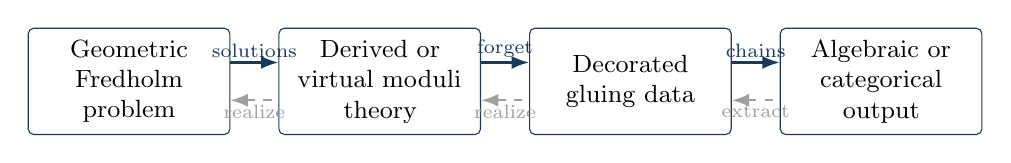
\begin{tikzpicture}[
  box/.style={draw=deepblue,rounded corners=2pt,fill=white,text width=2.35cm,minimum height=1.35cm,align=center,font=\small,inner sep=3pt},
  arr/.style={-{Latex[length=2.2mm]},thick,deepblue},
  inv/.style={{Latex[length=2.2mm]}-,thick,dashed,gray!75},
  lab/.style={font=\scriptsize,inner sep=1.5pt}]
\node[box,anchor=west] (pde) at (0,0) {Geometric\\Fredholm\\problem};
\node[box,anchor=east] (alg) at (\textwidth,0) {Algebraic or\\categorical\\output};
\node[box] (mod) at ($(pde.center)!1/3!(alg.center)$) {Derived or\\virtual moduli\\theory};
\node[box] (deg) at ($(pde.center)!2/3!(alg.center)$) {Decorated\\gluing data};
% forward arrows (upper lane) and inverse, dashed arrows (lower lane)
\draw[arr] ([yshift=2.4mm]pde.east) -- node[lab,above]{solutions} ([yshift=2.4mm]mod.west);
\draw[inv] ([yshift=-2.4mm]pde.east) -- node[lab,below]{realize} ([yshift=-2.4mm]mod.west);
\draw[arr] ([yshift=2.4mm]mod.east) -- node[lab,above]{forget} ([yshift=2.4mm]deg.west);
\draw[inv] ([yshift=-2.4mm]mod.east) -- node[lab,below]{realize} ([yshift=-2.4mm]deg.west);
\draw[arr] ([yshift=2.4mm]deg.east) -- node[lab,above]{chains} ([yshift=2.4mm]alg.west);
\draw[inv] ([yshift=-2.4mm]deg.east) -- node[lab,below]{extract} ([yshift=-2.4mm]alg.west);
\end{tikzpicture}
\caption{The forward construction and the three inverse questions.  Dashed arrows denote realization problems, not canonical inverse functors.}
\label{fig:program}
\end{figure}

The backward arrows in Figure~\ref{fig:program} are dashed because they are not inverse functors.  An algebra generally has many presentations, decorated gluing data can admit inequivalent geometric realizations, and a moduli space can arise from distinct equations.  The relevant questions concern existence, classification, and obstruction.

\section{The inverse moduli problem}\label{sec:formal}

\subsection{Algebra, gluing data, moduli theories, and Fredholm problems}

For a first formal model, consider four classes of objects.
\begin{description}[leftmargin=2.6cm,style=nextline]
\item[\(\Alg\)] Chain complexes with operations and relations, including \(\Ainf\), \(L_\infty\), BV, Frobenius, CohFT, operadic, properadic, or higher-categorical data.
\item[\(\Deg\)] Typed combinatorial systems describing dimensions, admissible splittings and gluings, automorphisms, signs, labels, and higher compatibility among strata.
\item[\(\GeomMod\)] Coherent families of compactified smooth, orbifold, Kuranishi, polyfold, or derived moduli objects with evaluation maps and gluing collars.
\item[\(\FredProb\)] Geometric analytic problems with their background geometry, fields, symmetries, boundary or asymptotic conditions, gauge fixing, Fredholm deformation theory, perturbations, energy control, compactness, orientations, and gluing analysis; elliptic and gradient-flow equations are the principal examples.
\end{description}

These names are used schematically in this section and the next.  For the boundary branch, Section~\ref{sec:comparison} replaces \(\Deg\) by the category of boundary-type gluing data, \(\GeomMod\) by derived orbifolds with corners, and the map between them by a Grothendieck construction.  No categorical model for \(\Alg\) or \(\FredProb\) is fixed here.  Each assertion below specifies the level at which it is made.

\subsection{Decorated Feynman-category gluing data}

The terminology has a concrete interpretation in the examples.  For planar operations, an elementary operation type is a corolla, a one-comma generator is a one-vertex operation, and a factorization is a tree obtained by composing such vertices.  Contracting an internal edge composes the adjacent operations and moves from a deeper boundary stratum toward the interior.  Stable graphs give the corresponding modular example, with internal edges representing nodes.  Definition~\ref{def:grammar} records this standard Feynman-category structure together with the geometric decorations needed below.

\begin{definition}[Decorated gluing datum]\label{def:grammar}
A \emph{decorated gluing datum} \(\Gamma\) consists of:
\begin{enumerate}
\item a decorated Feynman category \(\mathfrak F_\Gamma=(\mathcal V_\Gamma,\mathcal F_\Gamma,\iota_\Gamma)\), in which \(\mathcal V_\Gamma\) is the groupoid of elementary operation types and morphisms of \(\mathcal F_\Gamma\) encode substitution and gluing;
\item an additive virtual-dimension function on elementary operation types and an additive energy map to a commutative ordered monoid;
\item an orientation line, equivariant under automorphisms, for every elementary operation type;
\item for each elementary type \(v\), the factorization category \(\Fact_\Gamma(v)\), whose objects are factorizations of morphisms with target \(\iota_\Gamma(v)\) into tensor products of one-comma generators (the morphisms with a single target vertex), including the length-one factorization, and whose arrows contract internal composites; and
\item a codimension functor \(\Fact_\Gamma(v)\to\mathbb N\), equal to the number of independent internal gluings and compatible with substitution and tensor product.
\end{enumerate}
Decorations of the Feynman category may record curve classes, markings, tangency conditions, or evaluation targets.  The hereditary axiom (every morphism decomposes, uniquely up to the stated isomorphisms, into a tensor product of one-comma generators) makes item (4) well defined up to those isomorphisms~\cite{kaufmannward2017,kaufmannlucas2017}.  \end{definition}

For a one-edge boundary gluing with factors \(\alpha_i\), dimension consistency has the numerical form
\begin{equation}\label{eq:dim-consistency}
 d(\alpha)-1=\sum_i d(\alpha_i)-\dim G_{\mathrm{match}},
\end{equation}
where the final term accounts for matching constraints.  A gluing datum is \emph{chain coherent} if its signed codimension-two decompositions cancel in pairs, the combinatorial precursor of \(\partial^2=0\).  It is \emph{geometrically coherent} only if those identities can be upgraded to compatible collars, corners, isotropy, and orientations.

Iterating elementary morphisms produces trees, graphs, or buildings, while the resulting formal object remains a decorated Feynman category.  Definitions~\ref{def:ccf} and~\ref{def:smoothing-profile} impose the additional conditions governing boundary incidence and local smoothing geometry.

\subsection{Three inverse problems}

\begin{problem}[Extraction of gluing data from an algebra]\label{prob:i1}
Given \(B\in\Alg\), classify gluing data \(\Gamma\in\Deg\) and chain-level realization maps \(A(\Gamma)\to B\).  Determine which features of \(\Gamma\) are forced by \(B\), which depend on a presentation of \(B\), and which cannot be recovered from \(B\).
\end{problem}

No reconstruction theorem is expected at this level.  Homology forgets chain-level and geometric data, while quasi-isomorphic algebras can have different presentations.  A useful formulation may therefore begin with a cofibrant resolution or a Feynman transform of the algebra.

\begin{problem}[Geometric realization]\label{prob:i2}
Given \(\Gamma\in\Deg\), determine whether there is a coherent family \(\{\overM_\alpha\}\in\GeomMod\) such that its codimension-one and iterated boundary strata realize the decomposition rules of \(\Gamma\).  If so, classify realizations up to an appropriate concordance or derived equivalence.
\end{problem}

Equivalently, the problem is to characterize the essential image of
\[
 D:\GeomMod\longrightarrow\Deg.
\]
Even a regular CW complex with the desired face poset may be insufficient: one needs local models, compatible product collars, orientations, and often evaluation maps and virtual tangent data.

\begin{problem}[Fredholm realization]\label{prob:i3}
Given \(\mathfrak M\in\GeomMod\), determine whether it is represented, after perturbation or derived enhancement, by the solution theory of a natural geometric problem with Fredholm deformation theory.  Equivalently, characterize the essential image of
\[
 P:\FredProb\longrightarrow\GeomMod.
\]
\end{problem}

Here ``natural'' requires a mathematical explanation.  Without locality, covariance, or geometric functoriality, arbitrary finite-dimensional zero sets can be encoded artificially as equations.  A candidate should identify the underlying geometric structures, explain why the fields and symmetries belong to them, and state the locality, variational, energy, or physical principle that selects the equation.  No one type of justification is required: a variational formulation may be unavailable, and a physical interpretation may be conjectural.  What is required is an analytic explanation of the prescribed degenerations and a geometric reason to study the equation beyond its encoding of a chosen zero locus.

\subsection{Loss of information and nonuniqueness}

Each forward arrow in \eqref{eq:forward-cats} forgets information.  Passing from a geometric Fredholm source to a moduli object forgets much of the ambient field theory and analytic presentation.  Passing to a gluing datum forgets smooth structure inside strata, evaluation maps, characteristic classes, and metric information.  Passing to algebra may forget all chain-level structure beyond a chosen invariant.

Consequently, inverse moduli theory has two outputs even when construction fails:
\begin{enumerate}
\item \emph{realizability obstructions}, which prove that no object at the preceding layer can map to the prescribed datum; and
\item \emph{moduli of realizations}, which measure nonuniqueness when lifts do exist.
\end{enumerate}
This is analogous to lifting problems throughout topology: the relevant object is often a homotopy fiber of a forgetful functor, not a set-theoretic inverse.

\section{Marked realizations and their fibers}\label{sec:comparison}

This section defines the comparison object and its realization fibers.  The provisional map
\[
  D:\GeomMod\longrightarrow\Deg
\]
cannot be defined on an unmarked geometric moduli theory.  A family of stratified spaces can admit inequivalent identifications of its boundary strata with compositional types.  Even when the underlying face posets agree, labels, energy classes, automorphism weights, and orientations can encode different algebra.  We therefore include the combinatorial structure as a \emph{marking} of a geometric realization.

For the boundary-type branch, the appropriate comparison object is a category of pairs \((\Gamma,X)\), where \(\Gamma\) is specified operadic or Feynman-categorical gluing data and \(X\) is a compatible system of derived orbifolds with corners.  The forgetful map to gluing data is then the projection \((\Gamma,X)\mapsto\Gamma\), and its homotopy fiber is the space of realizations of that fixed gluing datum.  Sections~\ref{sec:complex-local-model}--\ref{sec:change-grammar} enlarge the combinatorial input by a local smoothing profile so that the same construction can be stated relative to other geometric targets.

\subsection{Corner models}

We first isolate the local combinatorics of corners.  The following definition is the convention of \namecite{Abouzaid and Blumberg}{abouzaidblumberg2024}, where such a \(P\) is called a \emph{model for manifolds with corners}.

\begin{definition}[Category modeling corners]\label{def:corner-model}
A \emph{category modeling corners} is a small category \(P\) equipped with a functor
\[
 \operatorname{codim}:P\longrightarrow\mathbb N
\]
such that, for every \(p\in P\), the overcategory \(P_{/p}\) is isomorphic to the Boolean lattice of subsets of a set with \(\operatorname{codim}(p)\) elements.  A \(P\)-stratification of an orbifold with corners \(X\) is a codimension-preserving functor from the face category of \(X\) to \(P\) that induces an isomorphism on the overcategory of every face.
\end{definition}

The Boolean condition is local.  Globally, different faces may carry the same label, which is why a category is used instead of a poset.  The isomorphism condition is nevertheless rigid.  Since a Boolean lattice is skeletal, no two distinct objects of \(P_{/p}\) are isomorphic, and every \(\sigma\in\operatorname{Aut}(p)\) is the identity.  Thus a category modeling corners has trivial automorphism groups.  Isotropy must be recorded separately from \(P\): Definition~\ref{def:normal-exact} and Proposition~\ref{prop:stable-graphs} place automorphism actions on the indexed objects, not on the indexing category.  Products of corner models supply the symmetric monoidal structure needed for products of moduli spaces.

Definition~\ref{def:corner-model} is more precise than the incidence data in Definition~\ref{def:grammar}.  It records the local orthant structure of an actual manifold or orbifold with corners.  A gluing datum whose factorization categories fail this local Boolean condition cannot be realized in this target without enlarging the allowed singularity class.  Conversely, Boolean incidence alone does not imply that the local smoothing parameters are boundary coordinates; this distinction becomes important for stable complex curves below.

\subsection{The combinatorial source}

Fix a symmetric monoidal category \(\mathcal C\).  Recall that an algebra over a Feynman category \(\mathfrak F=(\mathcal V,\mathcal F,\iota)\) with values in \(\mathcal C\) is a strong symmetric monoidal functor \(\mathcal F\to\mathcal C\)~\cite{kaufmannward2017}.  Definition~\ref{def:grammar} fixes the decorated Feynman-categorical source used throughout.  For the boundary target, it must satisfy the following additional condition.

\begin{definition}[Boundary-type corner-compatible gluing datum]\label{def:ccf}
A decorated gluing datum \(\Gamma\) is \emph{boundary-type and corner-compatible} when:
\begin{enumerate}
\item every \(\Fact_\Gamma(v)\) is a category modeling corners in the sense of Definition~\ref{def:corner-model};
\item tensor product corresponds to the product of corner models;
\item contraction and substitution preserve virtual dimension, energy, automorphism actions, and orientation lines; and
\item every elementary degeneration has real virtual codimension one.
\end{enumerate}
This applies Abouzaid and Blumberg's corner condition~\cite{abouzaidblumberg2024} to the factorization categories; it is an additional condition on a Feynman category.  Retaining the length-one factorization in Definition~\ref{def:grammar} makes the corolla an object of \(\Fact_\Gamma(v)\); without it, the overcategory at a one-edge factorization would not be the Boolean lattice on one element.
\end{definition}

This condition should be distinguished from cubicality, although the two agree in the graph examples below.  Kaufmann and Ward call a graded Feynman category \emph{cubical} when its degree function is proper, so that degree zero means isomorphism, and when a free symmetric-group action on maximal factorization chains identifies their coinvariants with the morphism sets~\cite{kaufmannward2017,kaufmannward2023koszul}.  Corner-compatibility instead requires the entire overcategory to be a Boolean lattice, with a unique arrow for every inclusion of subsets.  Cubicality controls only the maximal chains and does so up to isomorphism; its factorization structure is a torsor, not a strict lattice, and may degenerate in the presence of automorphisms.  Cubicality also requires properness and additivity of degree under the monoidal product, neither of which is assumed here.  Hence the two notions agree for the tree and graph examples used below but are not equivalent in general.

In the tree models, \(\Fact_\Gamma(v)\) is the category of trees resolving a corolla of type \(v\), and contracting internal edges moves from deeper corners toward the interior.  The local Boolean condition says that any subset of \(k\) independent breakings can be smoothed.  The corresponding local parameter lies in \([0,\varepsilon)^k\).

Let \(\BGrm\) denote the category whose objects are boundary-type corner-compatible gluing data.  A morphism
\[
 f:\Gamma\longrightarrow\Gamma'
\]
is a strong symmetric monoidal functor of the underlying decorated Feynman categories that preserves dimension, energy, orientations, and automorphism actions and is equipped, for every elementary \(v\), with a codimension-preserving isomorphism
\(
\Fact_\Gamma(v)\xrightarrow{\cong}\Fact_{\Gamma'}(f(v))
\)
compatible with tensor product, contraction, and substitution.  Every edge has the canonical boundary profile, so these are precisely the boundary-profile-preserving morphisms generalized in Definition~\ref{def:profile-morphism}.  More general changes of gluing data require Kan-extension hypotheses and are deferred.

\subsection{The geometric target}

Fix a tangential structure \(\theta\).  We use the relative notion of Abouzaid and Blumberg.  Merely imposing a structure on the virtual tangent class \(TU-E\) would add no constraint, since stabilizing \(TU\) by an auxiliary bundle gives every derived orbifold a tautological structure of that kind.  Instead, fix a pair of auxiliary bundles \((V_0,V_1)\).  A \(\theta\)-structure on a chart is a stable isomorphism from its virtual tangent bundle to a virtual bundle carrying the specified structure, together with \emph{consistent normal framings} of the corner strata.  The space of consistent normal framings extending fixed ones is contractible, so the transport in Theorem~\ref{thm:stabilization-normal} is well defined.  The cases used below are orientation, stable framing, and stable complex structure.

Let
\[
 \dOrb_\theta^{\mathrm{prop}}
\]
denote a symmetric monoidal category of proper, stratified derived orbifolds with corners and \(\theta\)-structure in this sense, with all charts indexed by the fixed pair \((V_0,V_1)\).  Concretely, a chart consists of an effective paracompact orbifold with corners \(U\), an obstruction bundle \(E\to U\), and a section \(s\) with compact zero locus.  Products use products of orbifolds and direct sums of obstruction bundles.  A morphism of charts consists of a map of the underlying orbifolds with corners and a bundle map intertwining the sections, in the sense of Abouzaid--Blumberg.  The arrows in Definition~\ref{def:marked-realization}(2) are the boundary inclusions among these morphisms.

Let \(W\) be the class of \emph{strong equivalences} of~\cite{abouzaidblumberg2024}: zero-section inclusions into stabilizations, with the bundle structure included in the datum.  This class contains the chart isomorphisms and is closed under composition and products.  Indeed, the product of stabilizations by \(\mathcal K_1\) and \(\mathcal K_2\) is the stabilization by \(\operatorname{pr}_1^*\mathcal K_1\oplus\operatorname{pr}_2^*\mathcal K_2\).  We impose the marked normal data at the chart level and then localize at \(W\).  Other virtual theories require a comparison functor before they can replace this model.

This choice follows the derived-orbifold and flow-category framework of \namecite{Abouzaid and Blumberg}{abouzaidblumberg2024}.  It is not asserted to subsume every Gromov--Witten or gauge-theoretic foundation.  In particular, implicit atlases~\cite{pardon2016}, Kuranishi systems compatible with corners~\cite{fooo2020}, and polyfold Fredholm structures retain different data.  Accordingly, realization is indexed by the chosen virtual target.

\begin{definition}[Marked geometric realization]\label{def:marked-realization}
Let \(\Gamma\in\BGrm\).  A \emph{\(\theta\)-structured marked geometric realization} of \(\Gamma\) is a strong symmetric monoidal functor
\begin{equation}\label{eq:realization-functor}
 X:\mathcal F_\Gamma\longrightarrow
 \dOrb_\theta^{\mathrm{prop}}
\end{equation}
satisfying the following conditions.
\begin{enumerate}
\item For each elementary type \(v\), the derived orbifold \(X(v)\) is stratified by \(\Fact_\Gamma(v)\).
\item A morphism represented by a one-edge gluing graph is carried to an isomorphism of charts from the corresponding product of lower moduli objects onto the labeled codimension-one corner stratum of \(X(v)\).
\item The composite gluing maps agree, up to specified coherent homotopies, with the identifications of higher-codimension corners supplied by the stratification in (1) and by edge contraction; when they agree on the nose, we say that the corner compatibilities of \(X\) hold strictly.
\item Every codimension-one corner stratum of \(X(v)\) occurs from an elementary factorization in \(\Gamma\).
\item At the stratum indexed by a factorization \(T\), the corner-normal object splits into the labeled inward real half-lines indexed by the internal edges of \(T\), with compatible collars under contraction and substitution.
\item Virtual dimensions, energy, automorphism actions, and orientation lines agree with the decorations of \(\Gamma\).
\end{enumerate}
\end{definition}

Conditions (2)--(4) will be called \emph{boundary exactness}.  The term means that the marked gluing datum is neither missing an actual boundary stratum nor adding a formal stratum absent from the compactification.  Boundary exactness is stronger than the existence of composition maps.

Condition (5) is the boundary instance of normal exactness, formulated for general local smoothing types in Definition~\ref{def:normal-exact}.  It is imposed before localization because collars and labeled normal lines are properties of representatives, not of bare objects in \(\dOrb_\theta^{\mathrm{prop}}[W^{-1}]\).

\subsection{The realization space}

Let \(\mathcal R_\theta(\Gamma)\) be the category of functors satisfying Definition~\ref{def:marked-realization}.  Its morphisms are monoidal natural transformations compatible with the marked strata, normal splittings, collars, and decorations.  Let \(W_\Gamma\) be the wide subcategory of transformations that are objectwise strong equivalences.  The notation \(\mathcal L_{W_\Gamma}\) denotes simplicial, equivalently Dwyer--Kan, localization~\cite[\S\S1.1--1.2]{hinich2016}.

\begin{definition}[Realization space]\label{def:real-space}
For \(\Gamma\in\BGrm\) and tangential structure \(\theta\), define
\begin{equation}\label{eq:real-space}
 \Real_\theta(\Gamma)
 :=
 \left(\mathcal L_{W_\Gamma}
 \mathcal R_\theta(\Gamma)\right)^{\simeq}.
\end{equation}
Here \(\mathcal L_{W_\Gamma}\) denotes the \(\infty\)-categorical localization of the nerve of \(\mathcal R_\theta(\Gamma)\) at \(W_\Gamma\) in \(\mathsf{Cat}_\infty\).  A construction through a simplicial model requires fibrant replacement before taking the core.  Points of the resulting space are marked realizations, and higher simplices record coherent higher equivalences.  Zigzags of objectwise strong equivalences map to paths in the core but do not constitute a literal description of it.
\end{definition}

The order of construction matters.  We first impose normal exactness on chart-level representatives and then localize.  Proposition~\ref{prop:target-localization} proves that the arrows inverted in \(W_\Gamma\) are themselves arrows of \(\mathcal R_\theta(\Gamma)\), so \eqref{eq:real-space} is the core of the localization of a genuine relative category.  Whether this core agrees with one defined intrinsically inside an already localized target is a separate question.

Thus \(\pi_0\Real_\theta(\Gamma)\) is the set of equivalence classes of realizations, while higher homotopy groups record automorphisms and families of equivalences.  In particular, nonemptiness is only the first inverse-moduli question.

The assignment \(\Gamma\mapsto\Real_\theta(\Gamma)\) is contravariant for the morphisms of \(\BGrm\) defined above.  At the relative-category level, the pullback construction later generalized in Proposition~\ref{prop:grammar-invariance} gives a normalized contravariant pseudofunctor
\[
 \Gamma\longmapsto\bigl(\mathcal R_\theta(\Gamma),W_\Gamma\bigr)
\]
from the ordinary category \(\BGrm\) to relative categories.  For composable morphisms \(\Phi:\Gamma\to\Gamma'\) and \(\Psi:\Gamma'\to\Gamma''\), its compositor is the relative natural isomorphism
\begin{equation}\label{eq:pullback-compositor}
 \mathbf c_{\Phi,\Psi}:\Phi^*\Psi^*\xRightarrow{\ \cong\ }(\Psi\Phi)^*.
\end{equation}
It is induced by associativity of precomposition and by the composite factorization and profile comparisons.  The identity pullback is chosen to be the identity functor, and the compositors involving an identity are identities.  The cocycle condition for \(\mathbf c\) is the associativity coherence of those comparisons.

Form the ordinary Grothendieck construction of this pseudofunctor.  Its objects are pairs \((\Gamma,X)\) with \(X\in\mathcal R_\theta(\Gamma)\).  A morphism \((\Gamma,X)\to(\Gamma',X')\) is a morphism \(\Phi:\Gamma\to\Gamma'\) in \(\BGrm\), together with an arrow \(f:X\to\Phi^*X'\).  For \((\Psi,g):(\Gamma',X')\to(\Gamma'',X'')\), composition is
\begin{equation}\label{eq:grothendieck-composition}
 (\Psi,g)\circ(\Phi,f)
 =\bigl(\Psi\Phi,\mathbf c_{\Phi,\Psi,X''}\circ\Phi^*g\circ f\bigr).
\end{equation}
The cocycle and unit identities for \(\mathbf c\), together with its naturality, make this composition associative and unital.  Declaring the weak equivalences to be the arrows lying over an identity and belonging to the corresponding \(W_\Gamma\) makes
\begin{equation}\label{eq:grothendieck}
 \int_{\Gamma\in\BGrm}\mathcal R_\theta(\Gamma)
\end{equation}
a relative category, and the projection to \(\BGrm\) is a relative functor when \(\BGrm\) carries only its identities as weak equivalences.  Localizing both sides gives
\begin{equation}\label{eq:shadow-corrected}
 D_\theta:
 \mathcal L\!\int_{\Gamma\in\BGrm}\mathcal R_\theta(\Gamma)
 \longrightarrow \BGrm,
 \qquad (\Gamma,X)\longmapsto\Gamma.
\end{equation}
Equation~\eqref{eq:shadow-corrected} is the precise replacement for the provisional forgetful functor.  Before localization the fiber of \eqref{eq:grothendieck} over \(\Gamma\) is, by construction, exactly the relative category \((\mathcal R_\theta(\Gamma),W_\Gamma)\) whose localization has core \(\Real_\theta(\Gamma)\).

It remains to compare the homotopy fiber of \eqref{eq:shadow-corrected} after localization with the localization of its fiber, whose core is \(\Real_\theta(\Gamma)\).  Section~\ref{sec:fiberwise-localization} proves this comparison for the Grothendieck construction.  The projection is a fibered category, its fiberwise weak equivalences form a saturated marking, and the localization theorem for families of \namecite{Hinich}{hinich2016} identifies the two fibers (Theorem~\ref{thm:fiberwise-localization}).  Sections~\ref{sec:examples}--\ref{sec:curved} do not use this result; their statements are fiberwise for a fixed gluing datum.  Thus \eqref{eq:shadow-corrected} gives a cartesian fibration from marked pairs to gluing data, but it does not extract canonical gluing data from a bare derived-orbifold system.

\subsection{Output theories}

A realization of a boundary gluing datum need not produce a prescribed algebra.  More importantly, the geometric target alone does not determine whether its natural output is a chain complex, a bordism class, or a spectrum.  This coefficient choice should therefore be part of the comparison problem.

\begin{definition}[Output theory]\label{def:output-theory}
For fixed \(\Gamma\), an \emph{output theory} with values in a symmetric monoidal \(\infty\)-category \(\mathcal C\) is a functor
\begin{equation}\label{eq:output-theory}
 \mathbb V_\Gamma:
 \mathcal L_{W_\Gamma}\mathcal R_\theta(\Gamma)
 \longrightarrow
 \operatorname{Alg}_{\mathfrak F_\Gamma}(\mathcal C)
\end{equation}
that converts the marked gluing identifications into the prescribed algebraic compositions.  Output theories for varying \(\Gamma\) are required to commute with pullback along morphisms of \(\BGrm\).
\end{definition}

If \(A\in\operatorname{Alg}_{\mathfrak F_\Gamma}(\mathcal C)\), define the output-refined realization space by
\begin{equation}\label{eq:refined-real}
 \Real_{\theta,\mathbb V}(\Gamma;A)
 :=\hofib_A\left(
 \Real_\theta(\Gamma)
 \xrightarrow{\ \mathbb V_\Gamma\ }
 \operatorname{Alg}_{\mathfrak F_\Gamma}(\mathcal C)^{\simeq}
 \right).
\end{equation}
Its points are marked geometric realizations together with a specified equivalence from their output to \(A\).  The extra equivalence is essential: two systems can have identical corner incidence and inequivalent outputs.  Formula~\eqref{eq:refined-real} also separates two obstructions that were conflated in the original schematic.  The space \(\Real_\theta(\Gamma)\) can be nonempty while \(\Real_{\theta,\mathbb V}(\Gamma;A)\) is empty, either because the required coefficient orientation fails or because the geometry realizes a different algebraic class.

A stabilization-invariant symmetric monoidal virtual-chain construction would give an example with \(\mathcal C=\Ch_R\).  Definition~\ref{def:output-theory} does not assume that such a construction exists.  In the unary flow case, the derived-orbifold framework instead supplies a bordism-theoretic output after the morphisms are enlarged from chart transformations to flow bimodules.  Thus the following proposition concerns the continuation-local realization space defined in \eqref{eq:flow-realization-space}, not automatically the chart-local category in \eqref{eq:output-theory}.

\begin{recollection}
Fix a tangential derived-orbifold bordism theory \(\theta\).  Let \(\operatorname{Flow}_\theta\) be the stable \(\infty\)-category of structured flow categories and flow bimodules, let \(*\) be its unit, and set
\begin{equation}\label{eq:bordism-ring-spectrum}
 \mathbb B_\theta
 :=\operatorname{Map}_{\operatorname{Flow}_\theta}(*,*).
\end{equation}
Then a structured flow category \(F\) has the equivalence-invariant output
\begin{equation}\label{eq:flow-spectrum}
 \mathbb H_\theta(F)
 :=\operatorname{Map}_{\operatorname{Flow}_\theta}(*,F),
\end{equation}
which is a module spectrum over the associative ring spectrum \(\mathbb B_\theta\).  Its homotopy groups are the bordism groups of \(F\).  In the framed case with trivial energy monoid, \(\operatorname{Flow}_{\mathrm{fr}}\simeq\mathsf{Sp}\) and \(\mathbb B_{\mathrm{fr}}\simeq\mathbb S\); the triviality hypothesis is used to make the unit a compact object, and is not automatic for the energy-graded gluing data considered here.
\end{recollection}

This recollection is due to Abouzaid and Blumberg~\cite{abouzaidblumberg2024}.  In particular, their results give the stability of \(\operatorname{Flow}_\theta\) with flow bimodules as morphisms, identify the homotopy groups of \eqref{eq:flow-spectrum} with the bordism groups of \(F\), construct the ring structure on \eqref{eq:bordism-ring-spectrum}, and prove the framed comparison.  Only the \(\mathbb B_\theta\)-module structure by precomposition is formal here.  We use this construction as the output theory for the flow case.

Ordinary chains require one additional choice.  A multiplicative orientation
\begin{equation}\label{eq:coefficient-orientation}
 \epsilon:\mathbb B_\theta\longrightarrow HR
\end{equation}
gives, in the flow case, the extension of scalars
\begin{equation}\label{eq:chain-base-change}
 \mathbb H_\theta(F)\otimes_{\mathbb B_\theta}HR
 \in\operatorname{Mod}_{HR}\simeq D(R).
\end{equation}
For framed bordism, \eqref{eq:coefficient-orientation} is the unit map \(\mathbb S\to HR\).  For derived orbifolds with isotropy or for higher Feynman-categorical operations, the required orientation and multiplicative refinement must be supplied separately.  The cited flow-category construction explicitly leaves general multiplicative spectral structures to subsequent work; it therefore does not justify a universal functor \(C_*^{\vir}\) on the target used above.

\subsection{Flow categories and associahedra}

\paragraph{Morse and Floer trajectories.}
For an object set \(P\) and an abelian monoid \(\Lambda\) with energy homomorphism to \([0,\infty)\), \namecite{Abouzaid and Blumberg}{abouzaidblumberg2024} construct a nonunital \(\Lambda\)-graded strict \(2\)-category whose morphism categories consist of labeled directed arcs and their internal-edge contractions.  These categories model corners.  A flow category is a nonunital category enriched in stratified derived orbifolds, with composition maps identifying products of trajectory spaces with the appropriate boundary strata.  A \emph{structured} flow category is a further lift along their tangential-structure fibration.

The unary directed specialization of Definition~\ref{def:marked-realization} should recover the object-level notion, but no comparison is proved here.  Their structured objects include index and normal-direction data absent from Definition~\ref{def:marked-realization}.  Moreover, flow bimodules provide the morphisms needed for a stable \(\infty\)-category, so the continuation-local construction below uses those morphisms instead of the chart transformations in \(\mathcal R_\theta(\Gamma)\).

\paragraph{Associahedra.}
Let \(\Gamma_{\mathrm{Ass}}\) be the planar rooted-tree gluing data.  With the convention that \(K_n\) parametrizes stable disks with \(n\) ordered inputs and one output, \(\dim K_n=n-2\).  The assignment
\[
 v_n\longmapsto K_n
\]
and grafting of trees define a boundary-exact realization in oriented manifolds with corners.  A facet indexed by \(r+s+t=n\) with \(s\geq2\) and \(r+1+t\geq2\) is
\[
 K_{r+1+t}\times K_s,
\]
and the oriented cellular-chain algebra satisfies the Stasheff identities.  Let
\(
A_K=C_*^{\mathrm{cell}}(K_\bullet;R)
\)
denote this \(\Ainf\)-algebra.  On the associahedral subcategory, oriented cellular chains define an output theory, and hence
\[
 K_\bullet\in
 \Real_{\mathrm{or},C_*^{\mathrm{cell}}}
 (\Gamma_{\mathrm{Ass}};A_K).
\]
This example shows that the definition captures higher compositions, but it does not yet reconstruct pseudoholomorphic polygons.  That further lift belongs to the elliptic-realization stage.

\subsection{Factorization categories for planar trees}

The first functoriality question admits an explicit description in the planar-tree case.  A \emph{stable planar rooted tree} with \(n\) inputs has \(n\) incoming leaves labeled in planar order, one outgoing root, and at least two incoming flags at every internal vertex.  Write \(E^{\mathrm{int}}(T)\) for its internal edges.

For \(n\geq 2\), define \(\mathsf{PT}_n\) as follows.  Its objects are isomorphism classes of stable planar rooted trees with \(n\) inputs.  For every tree \(T\) and subset \(I\subseteq E^{\mathrm{int}}(T)\), there is a morphism
\begin{equation}\label{eq:tree-arrow}
 T/I\longrightarrow T,
\end{equation}
where \(T/I\) is obtained by contracting the edges in \(I\).  These are all morphisms, and composition corresponds to union of contracted-edge sets.  Set
\[
 \operatorname{codim}(T)=|E^{\mathrm{int}}(T)|.
\]

\begin{proposition}[Planar-tree corner model]\label{prop:planar-corners}
The following statements hold.
\begin{enumerate}
\item Each \(\mathsf{PT}_n\) is a category modeling corners.
\item Grafting the root of \(S\in\mathsf{PT}_s\) to the \(i\)-th input of \(T\in\mathsf{PT}_r\) defines a functor
\[
 \circ_i:\mathsf{PT}_r\times\mathsf{PT}_s
 \longrightarrow\mathsf{PT}_{r+s-1}
\]
that raises codimension by one and identifies its source with the full subcategory of trees containing the distinguished grafting edge.
\item The grafting functors are associative and compatible with edge contraction.  Consequently, \(\{\mathsf{PT}_n\}_{n\geq2}\) is the system of factorization categories, in the sense of Definition~\ref{def:grammar}(4)--(5), of the nonsymmetric operadic gluing data for \(\Ainf\)-operations, and each of them models corners.
\end{enumerate}
\end{proposition}

\begin{proof}
Fix \(T\in\mathsf{PT}_n\).  An object of the overcategory \((\mathsf{PT}_n)_{/T}\) is precisely a contraction map \(T/I\to T\) of the form \eqref{eq:tree-arrow}.  Because the inputs are ordered and labeled, a stable planar rooted tree has no nontrivial automorphisms, so the passage to isomorphism classes is harmless and a contracted subset is recovered from this map.  A morphism between two such contractions is precisely an inclusion of the corresponding subsets.  Hence
\[
 (\mathsf{PT}_n)_{/T}\cong
 \mathcal P\bigl(E^{\mathrm{int}}(T)\bigr),
\]
the Boolean lattice on \(\operatorname{codim}(T)\) elements, under the identification \(I\mapsto E^{\mathrm{int}}(T)\setminus I\) that makes \(\operatorname{codim}\) monotone for the ordering of \(\mathbb N\) as a poset.  This proves (1).

Let \(T\circ_i S\) denote the grafted tree and let \(e_i\) be the new internal edge created by the graft.  There is a canonical disjoint union
\begin{equation}\label{eq:graft-edges}
 E^{\mathrm{int}}(T\circ_i S)
 \cong E^{\mathrm{int}}(T)\sqcup
 E^{\mathrm{int}}(S)\sqcup\{e_i\}.
\end{equation}
It follows that
\[
 \operatorname{codim}(T\circ_iS)
 =\operatorname{codim}(T)+\operatorname{codim}(S)+1.
\]
If \(I\subseteq E^{\mathrm{int}}(T)\) and
\(J\subseteq E^{\mathrm{int}}(S)\), then
\begin{equation}\label{eq:graft-contract}
 (T/I)\circ_i(S/J)
 \cong (T\circ_iS)/(I\sqcup J).
\end{equation}
Thus grafting is functorial for contraction maps.  For fixed \((r,s,i)\) the grafting edge is the unique internal edge whose subtree carries exactly the inputs \(i,\ldots,i+s-1\), uniqueness following from stability, so \(\circ_i\) is injective on objects; and no morphism between two objects of the image contracts \(e_i\), since contracting it destroys the unique edge with that leaf set.  The image is therefore the full subcategory of trees possessing such an edge, and contracting \(e_i\) leaves that boundary face.  Equations~\eqref{eq:graft-edges} and \eqref{eq:graft-contract} prove (2).

Finally, grafting planar rooted trees is associative after the canonical relabeling of ordered inputs.  Under the edge identification \eqref{eq:graft-edges}, the two iterated graftings have the same internal edges and the same contraction maps.  The associativity diagrams therefore commute, proving (3).
\end{proof}

The standard face-poset description of the associahedron~\cite{stasheff1963,markl2002} identifies \(\mathsf{PT}_n\) with the face category of \(K_n\): an internal edge records one nodal splitting and a \(k\)-edge tree labels a codimension-\(k\) face.  Proposition~\ref{prop:planar-corners} therefore proves factorization functoriality for the planar \(\Ainf\) example.  It does not prove the corresponding statement for graph categories with loops or automorphisms.  In those cases the factorization data are not indexed by a poset, and isotropy must be retained separately, since by the preceding remark a category modeling corners cannot carry it.

\subsection{Why stable complex curves require a different local model}\label{sec:complex-local-model}

The Boolean incidence of a degeneration does not determine its normal geometry.  Near a broken Morse trajectory or a nodal boundary disk, an elementary gluing parameter is a nonnegative real number.  The degenerate locus is therefore a real boundary hypersurface.  By contrast, a node of a stable complex curve has a local equation
\begin{equation}\label{eq:node-smoothing}
 xy=t,
 \qquad t\in\mathbb C.
\end{equation}
The nodal locus \(t=0\) is complex codimension one and real codimension two.  With \(k\) nodes, the local smoothing base is \(\mathbb C^k\), possibly modulo an automorphism group acting on the smoothing coordinates.  It is not an orthant \([0,\varepsilon)^k\), and the nodal locus is not a boundary face of a manifold with corners.  This is the local geometry underlying the stable-graph gluing of \(\overline{\mathcal M}_{g,n}\)~\cite{delignemumford1969,getzlerkapranov1998}.

Consequently, the CohFT example does not belong to \(\BGrm\) and is not a realization in \(\dOrb_\theta^{\mathrm{prop}}\) with its corner stratification.  The incidence category of stable graphs is still locally Boolean after rigidifying the graphs, but each edge carries a complex normal line rather than a real inward normal.  Automorphisms can also act nontrivially on these lines.

The general combinatorial source must therefore include a \emph{local smoothing model} in addition to a factorization category.  At a depth-\(k\) degeneration, this datum should distinguish at least
\begin{equation}\label{eq:local-models}
 \begin{array}{rcll}
 [0,\infty)^k &:& \text{boundary or breaking parameters},
 &\text{real codimension }k,\\
 \mathbb R^k &:& \text{transverse real strata},
 &\text{real codimension }k,\\
 \mathbb C^k &:& \text{nodal complex smoothing parameters},
 &\text{real codimension }2k,
 \end{array}
\end{equation}
together with the automorphism representation on the normal parameters and compatibility under composition.  A target-independent gluing datum can retain the common graph incidence, but realization must be relative to the chosen local smoothing model.  The corner construction of this section is the \([0,\infty)^k\) branch, not the universal case.

\subsection{Coordinate smoothing germs}

We now define the additional combinatorial datum.  Let the set of elementary local types be
\[
 \mathfrak T=\{\partial,\mathbb R,\mathbb C\},
\]
with basic pointed germs
\begin{equation}\label{eq:basic-germs}
 \mathbb D_\partial=([0,\infty),0),\qquad
 \mathbb D_{\mathbb R}=(\mathbb R,0),\qquad
 \mathbb D_{\mathbb C}=(\mathbb C,0).
\end{equation}
Their real codimension weights are \(w(\partial)=w(\mathbb R)=1\) and \(w(\mathbb C)=2\).

\begin{definition}[Category of coordinate smoothing germs]\label{def:smo-category}
The symmetric monoidal category \(\Smo\) has objects finite typed sets \((E,\tau)\), where \(\tau:E\to\mathfrak T\), representing the product germ
\begin{equation}\label{eq:smoothing-product}
 \mathbb D(E,\tau)=\prod_{e\in E}\mathbb D_{\tau(e)}.
\end{equation}
Morphisms are generated by type-preserving bijections, invertible linear changes within individual real or complex line factors (and positive rescaling of boundary factors), and coordinate projections
\[
 \pi_I:\mathbb D(E,\tau)\longrightarrow
 \mathbb D(E\setminus I,\tau|_{E\setminus I}).
\]
The monoidal product is disjoint union of typed sets, corresponding to product of pointed germs.
\end{definition}

Every object has a coordinate-zero stratification indexed by subsets of \(E\).  Definition~\ref{def:smo-category} deliberately excludes arbitrary mixing of coordinates: an elementary degeneration must remain identifiable under substitution.  If a theory has genuinely coupled smoothing directions, its local model lies outside \(\Smo\) and requires a larger target.

\begin{definition}[Smoothing profile]\label{def:smoothing-profile}
Let \(\Gamma\) be decorated Feynman-categorical gluing data with factorization categories \(\Fact_\Gamma(v)\).  A \emph{smoothing profile} on \(\Gamma\) is a collection of contravariant functors
\begin{equation}\label{eq:smoothing-functor}
 \nu_v:\Fact_\Gamma(v)^{\mathrm{op}}\longrightarrow\Smo
\end{equation}
with the following properties.
\begin{enumerate}
\item If a factorization \(T\) has elementary gluing edges \(E(T)\), then
\[
 \nu_v(T)=\mathbb D(E(T),\tau_T)
\]
for an automorphism-equivariant type function \(\tau_T:E(T)\to\mathfrak T\).
\item If \(T/I\to T\) contracts \(I\subseteq E(T)\), then \(\nu_v\) sends it to the coordinate projection forgetting the factors in \(I\).
\item For every substitution with new gluing-edge set \(G\), there is a coherent isomorphism
\begin{equation}\label{eq:profile-substitution}
 \nu\bigl(T\circ(T_1,\ldots,T_m)\bigr)
 \cong \nu(T)\times\prod_{j=1}^m\nu(T_j)
 \times\prod_{e\in G}\mathbb D_{\tau(e)}.
\end{equation}
These isomorphisms are associative, symmetric-monoidal, and equivariant for automorphisms.
\end{enumerate}
\end{definition}

Let \(\LGrm\) denote gluing data equipped with a smoothing profile.  The boundary-type category \(\BGrm\) is the full subcategory in which every elementary edge has type \(\partial\).  The complex-nodal gluing datum for stable curves instead has type \(\mathbb C\) on every edge.

\begin{proposition}[Independent-degeneration product law]\label{prop:profile-product}
Let \((\Gamma,\nu)\in\LGrm\).  For a factorization \(T\), its real normal codimension is
\begin{equation}\label{eq:weighted-codim}
 \operatorname{codim}_{\mathbb R}(T)
 =\sum_{e\in E(T)}w\bigl(\tau_T(e)\bigr).
\end{equation}
Codimension is additive under independent products.  A substitution has the excess codimension contributed by its new gluing edges:
\begin{equation}\label{eq:substitution-codim}
 \operatorname{codim}_{\mathbb R}
 \bigl(T\circ(T_1,\ldots,T_m)\bigr)
 =\operatorname{codim}_{\mathbb R}(T)
 +\sum_j\operatorname{codim}_{\mathbb R}(T_j)
 +\sum_{e\in G}w(\tau(e)).
\end{equation}
Contraction of \(I\) removes exactly the corresponding normal factors and lowers real codimension by \(\sum_{e\in I}w(\tau(e))\).
\end{proposition}

\begin{proof}
The product decomposition \eqref{eq:profile-substitution} identifies the set of smoothing coordinates with the disjoint union
\[
 E(T)\sqcup\coprod_jE(T_j)\sqcup G.
\]
Equations~\eqref{eq:weighted-codim} and \eqref{eq:substitution-codim} follow by summing the weights.  The contraction statement follows because \(\nu\) carries contraction to the coordinate projection \(\pi_I\).
\end{proof}

\subsection{Normal data in a geometric realization}

The profile records the type of a normal direction, not its varying geometric line.  Let \(X_T\) be the stratum of a marked geometric system indexed by a factorization \(T\).  A \emph{normal line of type \(\partial\)} means an inward-pointing real half-line bundle; types \(\mathbb R\) and \(\mathbb C\) mean real and complex line bundles, respectively.

\begin{definition}[Normally exact realization]\label{def:normal-exact}
A marked stratified realization \(X\) of \((\Gamma,\nu)\in\LGrm\) is \emph{normally exact} if, for every stratum \(X_T\), it is equipped with:
\begin{enumerate}
\item line bundles \(L_e\to X_T\) of type \(\tau_T(e)\), for \(e\in E(T)\);
\item an equivariant identification of its normal object with their sum,
\begin{equation}\label{eq:normal-splitting}
 N_{X_T/X}\cong\bigoplus_{e\in E(T)}L_e;
\end{equation}
\item an equivariant collar, tubular, or formal gluing chart from a neighborhood of the zero section in \(N_{X_T/X}\) to a neighborhood of \(X_T\) in \(X\); and
\item coherent identifications under contraction and substitution that cover the coordinate projections and products in \(\nu\).
\end{enumerate}
The automorphism group of \(T\) acts on \eqref{eq:normal-splitting}, including both permutations of summands and its linear action on each line.
\end{definition}

For boundary type, Definition~\ref{def:normal-exact} is the usual compatible-collar requirement.  For complex type, it is a normal-crossing or toroidal local model, interpreted in the analytic, algebraic, or logarithmic category appropriate to the realization.  The latter relation between stable-graph incidence and toroidal geometry is standard in the tropicalization of \(\overline{\mathcal M}_{g,n}\)~\cite{abramovich2015}.

\subsection{The associahedral and stable-graph profiles}

For a stable planar tree \(T\), assign type \(\partial\) to every internal edge and set
\[
 \nu_{\mathrm{Ass}}(T)=[0,\infty)^{E^{\mathrm{int}}(T)}.
\]
Equation~\eqref{eq:graft-edges} is precisely the substitution isomorphism \eqref{eq:profile-substitution}.  The compatible collars of associahedra make \(K_\bullet\) a normally exact realization.  Proposition~\ref{prop:profile-product} reduces to the codimension formula proved in Proposition~\ref{prop:planar-corners}.

For the complex case, let \(\mathsf{SG}^{\mathrm{rig}}_{g,n}\) be the category of connected stable genus-decorated graphs with \(n\) labeled legs, each equipped with a total ordering of its vertices and of its flags, transported under edge contraction by the induced ordering on the merged vertex.  A rigidified graph has no nontrivial automorphisms, which is what makes the overcategories below Boolean.  Its arrows are generated by contraction of internal edges; a loop contraction raises the genus of its incident vertex by one.  For a graph \(G\), define
\begin{equation}\label{eq:stable-profile}
 \nu_{g,n}(G)=\mathbb C^{E(G)},
\end{equation}
and send contractions to coordinate projections.  Graph substitution identifies edge sets by disjoint union together with the new edges created by gluing, so \eqref{eq:stable-profile} satisfies Definition~\ref{def:smoothing-profile}.  Forgetting the rigidification produces the stable-graph groupoid; graph automorphisms act by permuting coordinates.

\begin{proposition}[Stable-graph smoothing profile]\label{prop:stable-graphs}
For every rigidified stable graph \(G\), the overcategory of \(\mathsf{SG}^{\mathrm{rig}}_{g,n}\) at \(G\) is the Boolean lattice on \(E(G)\), the grading being the number of edges rather than the real codimension; and \(\nu_{g,n}\) defines a complex smoothing profile compatible with modular-operadic gluing.  For the stratum of \(\overline{\mathcal M}_{g,n}\) indexed by a stable graph \(G\), the pullback of the normal bundle to the product of vertex moduli spaces has the canonical decomposition
\begin{equation}\label{eq:stable-normal}
 N_G\cong\bigoplus_{e=\{h,\bar h\}\in E(G)}
 L_h^\vee\otimes_{\mathbb C}L_{\bar h}^\vee,
\end{equation}
where \(L_h\) and \(L_{\bar h}\) are the cotangent lines at the two branches of the node.  This decomposition is equivariant under \(\operatorname{Aut}(G)\) and realizes the profile \(\nu_{g,n}\).
\end{proposition}

\begin{proof}
After rigidification, a contraction map into \(G\) is uniquely specified by a subset of \(E(G)\); inclusions of subsets give the morphisms between contractions.  Thus the overcategory at \(G\) is the Boolean lattice \(\mathcal P(E(G))\).  The disjoint-union formula for edges under graph substitution proves functoriality and the profile identity.

For an edge \(e=\{h,\bar h\}\), choose local parameters \(x\) and \(y\) on the two branches.  A first-order smoothing has equation \(xy=t_e\).  Under changes \(x'=ax+O(x^2)\) and \(y'=by+O(y^2)\), the normal tangent vector \(\partial/\partial t_e\) transforms by \((ab)^{-1}\).  It therefore lies canonically in
\[
 T_{q_h}C_h\otimes T_{q_{\bar h}}C_{\bar h}
 =L_h^\vee\otimes L_{\bar h}^\vee.
\]
Independent nodes give the direct sum in \eqref{eq:stable-normal}.  An automorphism of \(G\) permutes the nodes and acts on their branch tangent lines, proving equivariance.  Standard deformation and plumbing theory identifies these lines with the normal directions to the stable-curve stratum~\cite{acg2011,wolpert2013}.
\end{proof}

Proposition~\ref{prop:stable-graphs} gives the local normal data used in the CohFT example.  It does not construct a single geometric target containing both corner charts and formal complex-normal charts.  The planar and stable-curve examples instead share a typed profile while their realizations lie in different geometric categories.

\subsection{Type-preserving changes of gluing data}\label{sec:change-grammar}

A change of gluing data must preserve more than edge incidence.  In particular, a functor cannot change a boundary smoothing parameter into a complex parameter without an additional map of local geometric theories.

\begin{definition}[Profile-preserving morphism]\label{def:profile-morphism}
Let \((\Gamma,\nu)\) and \((\Gamma',\nu')\) be objects of \(\LGrm\).  A \emph{profile-preserving morphism}
\[
 (\Phi,\alpha):(\Gamma,\nu)\longrightarrow(\Gamma',\nu')
\]
consists of:
\begin{enumerate}
\item a strong symmetric monoidal functor
\(\Phi:\mathcal F_\Gamma\to\mathcal F_{\Gamma'}\) preserving the dimension, energy, orientation, and automorphism decorations;
\item for each elementary type \(v\), an \emph{isomorphism} of factorization categories
\[
 \Phi_v:\Fact_\Gamma(v)
 \xrightarrow{\ \cong\ }\Fact_{\Gamma'}(\Phi v)
\]
compatible with factorization, tensor product, and substitution; and
\item a symmetric-monoidal natural isomorphism of smoothing profiles
\begin{equation}\label{eq:profile-comparison}
 \alpha:\nu\xRightarrow{\ \cong\ }\Phi^*\nu'.
\end{equation}
\end{enumerate}
A \(2\)-morphism is an invertible monoidal natural transformation between the underlying functors that intertwines the factorization functors and \eqref{eq:profile-comparison}.
\end{definition}

The notation \(\Phi^*\nu'\) means restriction along the functors \(\Phi_v^{\mathrm{op}}\).  The requirement that \(\Phi_v\) be an isomorphism prevents new strata from appearing under pullback.  With only a functor into \(\Fact_{\Gamma'}(\Phi v)\), a pulled-back realization of \(\Gamma'\) could have codimension-one strata indexed by no factorization of \(\Gamma\), contrary to conditions (1) and (4) of Definition~\ref{def:marked-realization}.  For example, take \(\Gamma\) to have one ternary type and no nontrivial factorizations, let \(\Gamma'=\Gamma_{\mathrm{Ass}}\), and use the associahedral realization.  The interval \(K_3\) has two corner strata, neither marked by the source gluing datum.  Since \(\alpha\) is an isomorphism in \(\Smo\), it also preserves the type and number of local normal coordinates.  Edge contraction remains an internal arrow of a factorization category, not a change of gluing data.

\begin{proposition}[Category of profiled gluing data]\label{prop:profile-category}
Profiled gluing data, profile-preserving morphisms, and the \(2\)-morphisms of Definition~\ref{def:profile-morphism} form a \((2,1)\)-category \(\LGrm^{(2)}\).  Its homotopy-coherent nerve defines an \(\infty\)-category \({\LGrm}_\infty\), the mapping objects being nerves of groupoids and hence Kan complexes.  The planar-tree boundary profiles and the stable-graph complex profiles span full subcategories closed under substitution.
\end{proposition}

\begin{proof}
If \((\Phi,\alpha):(\Gamma,\nu)\to(\Gamma',\nu')\) and
\((\Psi,\beta):(\Gamma',\nu')\to(\Gamma'',\nu'')\), their composite has underlying functor \(\Psi\Phi\), composite factorization functors, and profile comparison
\[
 \nu\xRightarrow{\alpha}\Phi^*\nu'
 \xRightarrow{\Phi^*\beta}
 \Phi^*\Psi^*\nu''\cong(\Psi\Phi)^*\nu''.
\]
Associativity follows from associativity of functor composition and pullback of natural transformations.  Identity functors carry identity profile comparisons.  The stipulated \(2\)-morphisms are invertible and compose vertically and horizontally, giving a \((2,1)\)-category.  Because all \(2\)-morphisms are invertible, each mapping object is the nerve of a groupoid and hence a Kan complex, so the simplicial category is locally Kan and its homotopy-coherent nerve is an \(\infty\)-category.  Closure of the two stated subcategories follows because their substitutions preserve, respectively, type \(\partial\) and type \(\mathbb C\).
\end{proof}

Let \((\mathcal G,W_{\mathcal G})\) be a symmetric monoidal relative geometric category admitting the normal objects and local charts required by a fixed profile.  Write \((\mathcal R_{\mathcal G}(\Gamma,\nu),W_{\Gamma,\mathcal G})\) for the relative category of normally exact realizations and objectwise arrows in \(W_{\mathcal G}\), and write
\[
 \Real_{\mathcal G}(\Gamma,\nu)
\]
for the core of its localization.  Thus normal data are imposed before target equivalences are inverted.  This recovers \(\Real_\theta(\Gamma)\) when \((\mathcal G,W_{\mathcal G})=(\dOrb_\theta^{\mathrm{prop}},W)\) and every edge is of boundary type.

\begin{proposition}[Invariance under equivalence of gluing data]\label{prop:grammar-invariance}
A profile-preserving morphism \((\Phi,\alpha)\) induces a relative pullback functor
\[
 \Phi^*:\bigl(\mathcal R_{\mathcal G}(\Gamma',\nu'),W_{\Gamma',\mathcal G}\bigr)
 \longrightarrow
 \bigl(\mathcal R_{\mathcal G}(\Gamma,\nu),W_{\Gamma,\mathcal G}\bigr)
\]
and hence a map
\begin{equation}\label{eq:real-pullback}
 \Phi^*:\Real_{\mathcal G}(\Gamma',\nu')
 \longrightarrow\Real_{\mathcal G}(\Gamma,\nu).
\end{equation}
For composable profile-preserving morphisms, the canonical comparisons \(\mathbf c_{\Phi,\Psi}:\Phi^*\Psi^*\Rightarrow(\Psi\Phi)^*\) are relative natural isomorphisms satisfying the cocycle and unit identities.  Thus the relative categories and pullbacks form a normalized contravariant pseudofunctor.  If \((\Phi,\alpha)\) is an equivalence in \(\LGrm^{(2)}\), then \eqref{eq:real-pullback} is an equivalence of \(\infty\)-groupoids.
\end{proposition}

\begin{proof}
Given a realization \(X':\mathcal F_{\Gamma'}\to\mathcal G\), precomposition gives \(X'\Phi\).  The factorization isomorphisms \(\Phi_v\) mark its strata, and \(\alpha\) identifies their prescribed local smoothing germs.  Pulling back the normal lines, normal splittings, and local charts of \(X'\) therefore gives a normally exact realization of \((\Gamma,\nu)\).  Objectwise arrows in \(W_{\mathcal G}\) remain objectwise arrows in \(W_{\mathcal G}\), so this is a relative functor and descends to \eqref{eq:real-pullback}.

For \(\Phi\) followed by \(\Psi\), the two pullbacks have the same underlying precomposed geometric functor.  Their transported markings are identified by associativity of the composite factorization isomorphisms and by the canonical comparison between \(\Phi^*\Psi^*\nu''\) and \((\Psi\Phi)^*\nu''\).  This gives \(\mathbf c_{\Phi,\Psi}\); its components are isomorphisms of marked realizations.  The two composites in the cocycle condition agree because both are the associativity comparison for triple precomposition, and the identity comparisons are identities.  Hence the stated pseudofunctor is normalized.

If \(\Phi\) is an equivalence, choose a profile-preserving quasi-inverse \(\Psi\).  The unit and counit \(2\)-isomorphisms induce homotopies between \(\Psi^*\Phi^*\), \(\Phi^*\Psi^*\), and the respective identity functors.  Hence \(\Phi^*\) is an equivalence.
\end{proof}

Propositions~\ref{prop:profile-category} and \ref{prop:grammar-invariance} give functoriality under type-preserving changes of gluing data.  They do not define pushforward along a quotient of gluing data, deletion of operation types, or a change \(\partial\to\mathbb C\).  Such operations require Kan extensions or a functor between geometric targets and are not included in the equivalence relation.

\subsection{Localization in the boundary derived-orbifold target}\label{sec:target-localization}

It remains to show that the relative presentation used in Definition~\ref{def:real-space} is stable under the target equivalences.  For the present boundary branch, this follows directly from the local form of stabilization.  If \((U,E,s)\) is a derived-orbifold chart and \(\mathcal K\to U\) is an orbifold vector bundle, its stabilization is
\begin{equation}\label{eq:chart-stabilization}
 \left(\operatorname{Tot}(\mathcal K),
 q^*E\oplus q^*\mathcal K,
 q^*s\oplus\zeta_{\mathcal K}\right),
\end{equation}
where \(q:\operatorname{Tot}(\mathcal K)\to U\) is the projection and \(\zeta_{\mathcal K}\) is the tautological fiber coordinate.  The zero section is a strong equivalence from the original chart to \eqref{eq:chart-stabilization} in the sense used for derived orbifolds and flow categories~\cite{abouzaidblumberg2024}.

Stabilizing a whole realization requires more than stabilizing each chart separately.  Throughout this subsection and the next, \(X\) is a normally exact realization whose corner compatibilities, in the sense of Definition~\ref{def:marked-realization}(3), hold strictly; the associahedral realization and every realization in a rigid target (Definition~\ref{def:rigid-target}) are of this kind, as are the flow categories of~\cite{abouzaidblumberg2024}, whose composition is strictly associative.

\begin{definition}[Compatible stabilization data]\label{def:stabilization-datum}
Let \(X\) be as above.
\begin{enumerate}
\item A \emph{compatible stabilization datum} for \(X\) is a family \(\{\mathcal K_v\}\) of orbifold vector bundles, one on each \(X(v)\), equivariant for the automorphisms of every operation type, together with restriction identifications of \(\mathcal K_{v}\) on the stratum indexed by a factorization \(T\) with the external sum \(\boxplus_{a\in V(T)}\mathcal K_a\) under the marked identification of that stratum with \(\prod_a X(a)\), compatible under edge contraction and substitution.
\item The datum is \emph{collared} if it is further equipped, for every closed face \(F\) of every \(X(v)\), with an equivariant isomorphism
\begin{equation}\label{eq:collar-trivialization}
 \mathcal K_v|_{C_F}\cong\pi_F^*\bigl(\mathcal K_v|_F\bigr)
\end{equation}
over the marked collar \(\pi_F:C_F\to F\) of Definition~\ref{def:normal-exact}(3), restricting to the identity over \(F\), such that on the overlap of the collars of two faces the two isomorphisms agree with the product-collar identification at their common corner, and such that the restriction identifications are compatible with \eqref{eq:collar-trivialization}.
\item A system of connections \(\{\nabla_v\}\), one on each \(\mathcal K_v\), is \emph{compatible} with a collared datum if each \(\nabla_v\) is invariant under \(\operatorname{Aut}(v)\), restricts on the stratum indexed by \(T\) to the external sum of the \(\nabla_a\) under the restriction isomorphism, and is of product form in every marked collar, that is, equals \(\pi_F^*(\nabla_v|_F)\) under \eqref{eq:collar-trivialization} on a neighborhood of \(F\) in \(C_F\).
\item For an elementary type \(v\), let \(\below{v}\) be the set of types occurring as vertices of noncorolla factorizations of \(v\); it is downward closed, by the hereditary factorization structure of Definition~\ref{def:grammar}(4).  A \emph{datum below \(v\)} is a family \(\{\mathcal K_a\}_{a\in\below{v}}\) with restriction identifications satisfying every instance of the conditions in (1) whose types lie in \(\below{v}\).
\end{enumerate}
\end{definition}

For a single face an isomorphism \eqref{eq:collar-trivialization} exists, since the inclusion \(F\subset C_F\) is an equivariant homotopy equivalence; the compatibility at corners is a choice, and it is taken as part of the datum.  The zero family, with the identity collar identifications, is a collared compatible datum, and so are the trivial systems of Proposition~\ref{prop:additive-data}.  The extension problem for a prescribed datum is treated in Section~\ref{sec:stabilization-data}.

Write \(a\prec v\) if \(a\) occurs as a vertex of a noncorolla factorization of \(v\), and take the transitive closure.  The existence argument below assumes that this relation is well founded, that the marked face stratification of each \(X(v)\) is locally finite, and that the operation-type automorphism groups are finite.  These hypotheses hold for the stable planar gluing datum, where arity decreases at every vertex, and for the directed unary gluing datum, where the action interval strictly decreases under breaking.  They are not consequences of the definition of a general decorated Feynman category.

\begin{theorem}[Compatible connections and stabilization invariance]\label{thm:stabilization-normal}
Let \(X\) be a normally exact realization of a boundary-type profile in \(\dOrb_\theta^{\mathrm{prop}}\) with strict corner compatibilities, and let \(\{\mathcal K_v\}\) be a collared compatible stabilization datum.
\begin{enumerate}
\item For every compatible system of connections \(\{\nabla_v\}\), the objectwise stabilization \(\widetilde X\) defined by \eqref{eq:chart-stabilization} is normally exact.  Restriction along the zero sections recovers the marked normal data of \(X\), and stabilization preserves the virtual tangent class, virtual dimension, orientation data, and every labeled corner stratum.
\item If the relation \(\prec\) is well founded, the marked face stratifications are locally finite, and the automorphism groups of operation types are finite, then compatible systems exist, and they form a nonempty convex, hence contractible, space.
\end{enumerate}
\end{theorem}

\begin{proof}
Let \(U_T\subset U\) be the stratum marked by a factorization \(T\).  The corresponding stratum of the stabilized ambient chart is \(\operatorname{Tot}(\mathcal K|_{U_T})\).  Its corner-normal bundle is
\begin{equation}\label{eq:stabilized-normal}
 N_{\operatorname{Tot}(\mathcal K|_{U_T})/\operatorname{Tot}(\mathcal K)}
 \cong q^*N_{U_T/U}.
\end{equation}
Consequently, the labeled splitting
\(
N_{U_T/U}\cong\bigoplus_{e\in E(T)}L_e
\)
pulls back to the same splitting with summands \(q^*L_e\).  In particular, no new corner-normal direction is created by stabilization: the vertical directions of \(\mathcal K\) are tangent to both total spaces in \eqref{eq:stabilized-normal}.

For (1), fix a compatible system.  The marked collars of the stabilized charts come from the collar identifications.  The connection defines a splitting
\[
 0\longrightarrow q^*\mathcal K
 \longrightarrow T\operatorname{Tot}(\mathcal K)
 \longrightarrow q^*TU
 \longrightarrow0
\]
compatible with strata and collars; the transport of the tangential structure below uses this splitting as an actual isomorphism.

Over the collar \(C_F\) of a face, the identification \eqref{eq:collar-trivialization} exhibits \(\operatorname{Tot}(\mathcal K|_{C_F})\) as \(\operatorname{Tot}(\mathcal K|_F)\times[0,\varepsilon)\), a marked collar for \(\operatorname{Tot}(\mathcal K|_F)\).  On the neighborhood where the connection has product form, the stabilized chart \eqref{eq:chart-stabilization} is likewise the product of its restriction over \(F\) with the collar coordinate.

Agreement of the collar identifications on overlaps gives compatibility at corners.  The external-sum restrictions of the bundles and connections give the identifications in Definition~\ref{def:normal-exact}(4) under contraction and substitution, since pullback commutes with products, collar projections, edge permutations, and restriction to deeper strata.  Equivariance of the datum and invariance of the connections make these constructions equivariant.  Hence \(\widetilde X\) is normally exact, and restriction along the zero sections recovers the marked normal data of \(X\).

Next, in real equivariant \(K\)-theory,
\begin{align}
 T\operatorname{Tot}(\mathcal K)-\left(q^*E\oplus q^*\mathcal K\right)
 &\simeq q^*(TU\oplus \mathcal K)-q^*(E\oplus \mathcal K)\\
 &=q^*(TU-E).
\end{align}
The added bundle cancels between tangent and obstruction terms, so the virtual dimension is unchanged.  The stable isomorphism defining the \(\theta\)-structure on \((U,E,s)\) is carried to the stabilized chart by adding the identity on the stabilizing bundle.  The consistent normal framings extend because the space of such extensions is contractible, and the induced orientation line is transported with them.  Restriction to the zero section recovers the original data.  Chart isomorphisms preserve the same structures tautologically.  This proves (1).

For (2), construct the system by well-founded induction on the operation types.  Suppose \(\nabla_a\) has been chosen for every \(a\prec v\), forming a compatible system on those types.  On a stratum of \(X(v)\) indexed by a noncorolla factorization \(T\), prescribe the connection obtained by transporting \(\boxplus_{a\in V(T)}\nabla_a\) through the restriction isomorphism of the datum.

These prescriptions agree on intersections of closed faces.  For independent refinements, this follows from the symmetry and associativity of the external sum.  For nested refinements, it follows from the contraction and substitution compatibility of the datum, which identifies direct restriction to the deeper stratum with iterated restriction along the strict corner identifications.  We therefore obtain compatible connections on the restrictions of \(\mathcal K_v\) to all positive-codimension strata.

Pull the connection on each closed face \(F\) back to its collar \(C_F\) through \eqref{eq:collar-trivialization}.  On the overlap of two collars, the pullbacks agree on the product collar of their common corner.  Indeed, the lower connections \(\nabla_a\) are already of product form and the collar identifications agree there.  The pullbacks consequently define a connection \(\nabla_\partial\) on the union \(N\) of the marked collars, of product form in every collar.

By local finiteness, there is a smooth function \(\chi\) on \(U\) that equals \(1\) on the union of the half-width collars, is supported in \(N\), and is pulled back from the faces on those smaller collars.  For an arbitrary connection \(\nabla_0\) on \(\mathcal K_v\), set
\[
 \nabla_v:=\chi\nabla_\partial+(1-\chi)\nabla_0.
\]
This connection has the prescribed restrictions and is of product form near every face.  Averaging over the finite automorphism group makes it invariant without changing these properties, since the collars and the datum are equivariant.

For a minimal operation type, boundary exactness leaves no prescribed face restriction, so any invariant connection begins the induction.  Well-founded induction then supplies the full system.

Relative to the fixed collar identifications \eqref{eq:collar-trivialization}, invariance and the prescribed external-sum restrictions are affine conditions on the connection, since differences of connections are endomorphism-valued one-forms, and product form on some neighborhood of each face is a directed union of affine conditions, hence convex.  The space of compatible systems is therefore convex, and nonempty by the construction just given; hence it is contractible.
\end{proof}

\begin{proposition}[The relative realization category and stabilization]\label{prop:target-localization}
Let \(\Gamma\in\BGrm\).  The class \(W_\Gamma\) is a wide subcategory, the pair
\begin{equation}\label{eq:relative-realization-category}
 \left(\mathcal R_\theta(\Gamma),W_\Gamma\right)
\end{equation}
is a relative category, and profile-preserving pullback is a relative functor, hence descends to localizations.  If \(X\in\mathcal R_\theta(\Gamma)\) has strict corner compatibilities and \(\{\mathcal K_v\}\) is a collared compatible stabilization datum admitting a compatible system of connections, in particular any such datum when the hypotheses of Theorem~\ref{thm:stabilization-normal}(2) hold, then the objectwise stabilization of \(X\) along \(\{\mathcal K_v\}\) is again an object of \(\mathcal R_\theta(\Gamma)\), and the objectwise zero-section transformation is an arrow of \(W_\Gamma\).
\end{proposition}

\begin{proof}
The wide-subcategory assertion follows directly from the definition: identities and composites of objectwise strong equivalences are objectwise strong equivalences.  Precomposition by a profile-preserving morphism does not change the target components of a natural transformation, so it preserves objectwise strong equivalences and defines a relative functor.

Under the additional hypotheses, Theorem~\ref{thm:stabilization-normal}(1) carries a normally exact marked realization to another such realization while preserving every labeled stratum, normal splitting, collar, and decoration.  Restriction along the zero sections recovers the marked normal data.  Hence the zero-section transformation is a morphism of \(\mathcal R_\theta(\Gamma)\), objectwise a strong equivalence, and therefore an arrow of \(W_\Gamma\).
\end{proof}

Every relative category admits a simplicial localization; what the proposition supplies is the pair \eqref{eq:relative-realization-category} that Definition~\ref{def:real-space} presupposes.

The target has two relevant limitations.  Its chart category has no colimits, and none are used above: localization only inverts a class of arrows, and we do not compute mapping spaces in \(\mathcal L_{W_\Gamma}\mathcal R_\theta(\Gamma)\).  Moreover, \(\mathcal R_\theta(\Gamma)\) is not small, so all constructions are relative to a fixed universe.

Theorem~\ref{thm:stabilization-normal} and Proposition~\ref{prop:target-localization} identify the relative category for the boundary derived-orbifold branch and prove closure under compatible stabilization, with existence of the required connections in the stated well-founded, locally finite class.  They do not establish an analogous statement for the complex-normal branch, which requires a relative analytic, algebraic, or logarithmic target with its own stabilization theorem.

\subsection{A stabilization datum that does not extend: the pentagon obstruction}\label{sec:stabilization-data}

The zero family is a compatible stabilization datum, and compatible data are closed under direct sum.  The geometric questions concern prescribed nonzero data: whether data on lower operation types extend to higher types, and which chartwise stabilizations occur in a compatible family.  The first question has a bundle-extension obstruction, realized below on the associahedral model.  Additive set decorations give compatible trivial stabilizations of unbounded rank for the standard planar and directed gluing data.

Such families occur naturally in Floer homotopy theory.  For each pair of objects and each energy label, a structured flow category carries a stabilizing bundle on the moduli chart.  Under composition these bundles add externally, while the accompanying virtual vector space acquires a fixed correction summand~\cite[Defs.~2.35, 3.8]{abouzaidblumberg2024}.  Vector bundles on flow categories satisfy an analogous external-sum-with-correction condition~\cite[Def.~2.32]{blakeyporcelli2026}.  Disk-component-wise obstruction bundle data satisfy a direct-sum condition over disk components and admit an unconditional existence theorem in their setting~\cite[Def.~5.1, Thm.~5.4]{fooo2020}; a horn-level existence result appears in~\cite[Prop.~5.12]{abouzaidblumberg2024}.

In these constructions the bundles are chosen during the argument and may be enlarged at every stage.  Here the datum is fixed on the lower types, and the question is whether it extends.  The answer is negative in general, although enlargement can remove the obstruction (Remark~\ref{rem:doubling}).  This differs from two familiar obstructions.  Coherent orientations of Floer moduli spaces may require relative spin data~\cite{fooo2009,ekholmetnyresullivan2005}, and a flow category may fail to admit a framing~\cite{cohenjonessegal1995,cohen2020floer}.  Neither structure has the direct-sum enlargement operation available for stabilization data.

Fix a normally exact realization \(X\) with strict corner compatibilities, an elementary type \(v\) with \(v\notin\below{v}\), and a datum below \(v\) in the sense of Definition~\ref{def:stabilization-datum}(4); the additive construction of Proposition~\ref{prop:additive-data} uses constant coordinate identifications and does not need the strictness assumption.

\begin{lemma}[Glued boundary bundle]\label{lem:glued-boundary}
Let \(X\) be as above, \(v\) an elementary type with \(v\notin \below{v}\), and \(\{\mathcal K_a\}\) a datum below \(v\).  There is an \(\operatorname{Aut}(v)\)-equivariant vector bundle \(B_v\) on \(\partial X(v)\).  It is the colimit of the following diagram over the closed faces of \(X(v)\).  A face labeled by \(T\) is assigned the external sum \(\boxplus_{a\in V(T)}\mathcal K_a\), transported to that face through the marked identification of Definition~\ref{def:marked-realization}(2).  A corner inclusion is assigned the map induced by the restriction isomorphisms of the datum and associativity of the external sum.  For every noncorolla factorization \(T\), the restriction of \(B_v\) to a stratum labeled by \(T\) is identified with \(\boxplus_{a\in V(T)}\mathcal K_a\).
\end{lemma}

\begin{proof}
The gluing is indexed by the face category of \(X(v)\), not by \(\Fact_\Gamma(v)\): Definition~\ref{def:corner-model} permits distinct faces to carry the same label, and the stratification functor restricts to an isomorphism on the overcategory of every face, which supplies the local label-injectivity that the corner identifications use.  The boundary \(\partial X(v)\) is the union of the closed codimension-one faces, every one of which carries a label by condition (4) of Definition~\ref{def:marked-realization}, so the prescriptions cover the boundary; local triviality at a corner is supplied by the collars of Definition~\ref{def:normal-exact}(3).  It remains to check that the corner identifications are route independent, so that the diagram has a colimit that is a vector bundle.  A two-step restriction from a face into a deeper corner splits into three cases.  If the two additional edges lie in different factors of the face's product decomposition, the two orders of restriction agree by bifunctoriality of the external sum together with the coherence of the index shuffles.  If both lie in one factor \(X(b)\), route independence is the contraction condition of the datum's compatibility for \(b\in \below{v}\).  And comparing either route with the direct marked identification of the deep stratum is the substitution condition, together with the standing strictness convention.  Equivariance combines the datum's equivariance condition with condition (6) of Definition~\ref{def:marked-realization}, the automorphisms of \(v\) permuting the faces through their action on \(\Fact_\Gamma(v)\).
\end{proof}

\begin{proposition}[Extension criterion]\label{prop:extension-criterion}
In the setting of Lemma~\ref{lem:glued-boundary}, the datum below \(v\) extends across \(v\) (that is, to a datum on \(\below{v}\cup\{v\}\)) if and only if \(B_v\) extends to an \(\operatorname{Aut}(v)\)-equivariant vector bundle on \(X(v)\): an equivariant bundle \(\mathcal K_v\) with an equivariant isomorphism \(\mathcal K_v|_{\partial X(v)}\cong B_v\).  In particular, for charts with trivial isotropy and trivial \(\operatorname{Aut}(v)\): if \(w_1(B_v)\) does not lie in the image of \(H^1(X(v);\mathbb Z/2)\to H^1(\partial X(v);\mathbb Z/2)\), then no extension exists, and none exists after enlarging the datum below \(v\) by any system whose glued boundary bundle is orientable, an enlargement meaning the direct sum of data, with block-diagonal restriction isomorphisms.
\end{proposition}

\begin{proof}
Given \((\mathcal K_v,\alpha)\), define the restriction identification at every stratum of \(X(v)\) as \(\alpha\) followed by the identifications of Lemma~\ref{lem:glued-boundary}; the contraction instances of the compatibility condition at \(v\) are the Lemma's internal consistency, and the substitution instances its route independence.  Conversely, the face identifications of an extended datum agree on corner overlaps (that agreement is the compatibility condition at \(v\)), so they glue to an equivariant isomorphism \(\mathcal K_v|_{\partial X(v)}\cong B_v\).  For the characteristic-class condition: \(w_1\) is natural, so an extension forces \(w_1(B_v)\) into the image of restriction; and an enlargement replaces \(B_v\) by \(B_v\oplus C_v\) with \(C_v\) the glued bundle of the enlarging system, so \(w_1(B_v\oplus C_v)=w_1(B_v)+w_1(C_v)=w_1(B_v)\) when \(C_v\) is orientable.
\end{proof}

The obstruction depends on the restriction isomorphisms as well as on the underlying bundles.  Changing the isomorphisms in the lower datum can alter \(B_v\) by more than a direct summand and can create or remove the obstruction, as the next example shows.  In the stable range, extension of the underlying bundles asks whether the class of \(B_v\) lies in the image of \(KO(X(v))\to KO(\partial X(v))\).  We do not prove or use this stable reformulation below.

\begin{proposition}[Trivial compatible data from additive set decorations]\label{prop:additive-data}
Call an \emph{additive set decoration} of a gluing datum an assignment of a finite \(\operatorname{Aut}(v)\)-set \(S_v\) to each elementary type.  For each one-edge factorization \(T\) with vertices \(a,a'\), it includes an equivariant bijection
\[
 \sigma_T:S_a\sqcup S_{a'}\longrightarrow S_v
\]
whose induced identifications for iterated factorizations are independent of the order of refinement.

The stable planar gluing data have such a decoration: \(S_v\) is the set of internal gaps between consecutive inputs, and a gap of a composite belongs to the deepest vertex whose block contains the two adjacent inputs.  The unary directed gluing datum on \(P\), for a strictly order-preserving map \(g:P\to\mathbb Z\), gives a second example.  Here \(S_{(x,z)}\) is the integer interval from \(g(z)+1\) to \(g(x)\), and breaking partitions it into consecutive subintervals.

For any additive set decoration and any \(M\ge1\), define
\[
 \mathcal K_v:=\underline{\mathbb R}^{\,S_v\times\{1,\dots,M\}}.
\]
The coordinate bijections induced by \(\sigma\) give the restriction identifications.  They are well defined at strata of arbitrary depth by the order-independence hypothesis.  With the tautological collar identifications, this is a collared compatible stabilization datum for every normally exact realization of the gluing datum.  Because the identifications are constant, the compatibility conditions hold whether or not the corner compatibilities are strict.  The trivial coordinate bundles carry a compatible system of flat connections.

Consequently, for every \(M\), the localization defining \(\Real_\theta(\Gamma)\) inverts the simultaneous stabilization of every chart by the trivial bundle of rank \(M|S_v|\).  If every \(S_v\) is nonempty, as in both examples above, each realization is equivalent in the localization to arbitrarily large trivial thickenings.  Thus compatible trivial thickenings exist in unbounded rank, although the rank needed for a transversality construction remains problem-dependent.
\end{proposition}

\begin{proof}
The external sum of trivial bundles is the trivial bundle on the disjoint union of the index sets, so the coordinate bijections are isomorphisms of the required shape.  Order independence gives the contraction and substitution compatibilities, and equivariance follows from the equivariance of \(\sigma\).  The constant coordinate identifications preserve the flat connections and are unaffected by the coherent homotopies of Definition~\ref{def:marked-realization}(3).  The flat coordinate connections are of product form for the tautological collar identifications, so the last assertions follow from Theorem~\ref{thm:stabilization-normal}(1) and Proposition~\ref{prop:target-localization}, whose proofs use the strictness of corner compatibilities only through the restriction identifications, and so apply verbatim when these are constant.
\end{proof}

The \(M=1\) instance on the stable planar gluing datum, whose restriction identifications are the bijections of gaps, is called the \emph{gap datum}.

\begin{figure}[t]
\centering
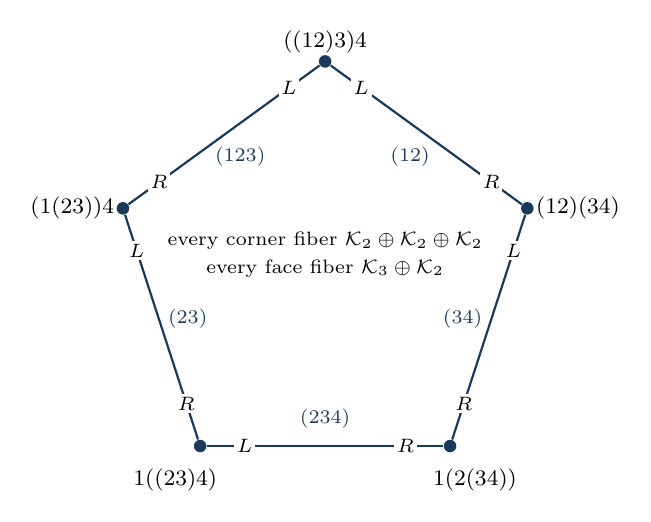
\begin{tikzpicture}[
  crn/.style={font=\footnotesize,inner sep=1pt},
  dot/.style={circle,fill=deepblue,inner sep=1.6pt},
  endmark/.style={font=\scriptsize,inner sep=1pt,fill=white},
  fac/.style={font=\scriptsize,color=deepblue,inner sep=1pt},
  edg/.style={thick,deepblue}]
\node[dot] (c1) at (90:2.7) {};
\node[dot] (c3) at (18:2.7) {};
\node[dot] (c5) at (306:2.7) {};
\node[dot] (c4) at (234:2.7) {};
\node[dot] (c2) at (162:2.7) {};
\node[crn,above=2pt] at (c1) {$((12)3)4$};
\node[crn,right=2pt] at (c3) {$(12)(34)$};
\node[crn,below=7pt,xshift=9pt] at (c5) {$1(2(34))$};
\node[crn,below=7pt,xshift=-9pt] at (c4) {$1((23)4)$};
\node[crn,left=2pt] at (c2) {$(1(23))4$};
\draw[edg] (c1) -- (c3);
\draw[edg] (c3) -- (c5);
\draw[edg] (c5) -- (c4);
\draw[edg] (c4) -- (c2);
\draw[edg] (c2) -- (c1);
\path (c1) -- (c3) node[endmark,pos=0.16]{$L$} node[endmark,pos=0.84]{$R$};
\path (c3) -- (c5) node[endmark,pos=0.16]{$L$} node[endmark,pos=0.84]{$R$};
\path (c4) -- (c5) node[endmark,pos=0.16]{$L$} node[endmark,pos=0.84]{$R$};
\path (c2) -- (c4) node[endmark,pos=0.16]{$L$} node[endmark,pos=0.84]{$R$};
\path (c1) -- (c2) node[endmark,pos=0.16]{$L$} node[endmark,pos=0.84]{$R$};
\node[fac] at ($($(c1)!0.5!(c3)$)!0.16!(0,0)$) {$(12)$};
\node[fac] at ($($(c3)!0.5!(c5)$)!0.16!(0,0)$) {$(34)$};
\node[fac] at ($($(c5)!0.5!(c4)$)!0.16!(0,0)$) {$(234)$};
\node[fac] at ($($(c4)!0.5!(c2)$)!0.16!(0,0)$) {$(23)$};
\node[fac] at ($($(c2)!0.5!(c1)$)!0.16!(0,0)$) {$(123)$};
\node[font=\scriptsize,align=center] at (0,0.25)
  {every corner fiber $\mathcal K_2\oplus\mathcal K_2\oplus\mathcal K_2$\\[2pt]
   every face fiber $\mathcal K_3\oplus\mathcal K_2$};
\end{tikzpicture}
\caption{The boundary of the pentagon \(K_4\).  The corners are the complete bracketings of four inputs.  Each face is labeled by its bracketed block, with endpoints marked \(L\) for \((xy)z\) and \(R\) for \(x(yz)\).  When \(\mathcal K_2=\mathbb R\) and \(\mathcal K_3=\mathbb R^2\), all corner and face fibers have rank three.  For the gap datum, every transition preserves the three gap labels, so the boundary monodromy is trivial.}
\label{fig:pentagon}
\end{figure}

\begin{theorem}[A sign twist on the pentagon]\label{thm:pentagon-twist}
Take \(\Gamma_{\mathrm{Ass}}\) with the associahedral realization \(X(n)=K_n\).  After choosing trivializations, a datum below arity \(4\) with \(\mathcal K_2\) of rank one consists of \(\mathcal K_2=\mathbb R\), \(\mathcal K_3=\mathbb R^2\), and two arbitrary isomorphisms
\[
 \varphi_L:\mathcal K_3|_{(xy)z}\to\mathcal K_2\oplus\mathcal K_2,
 \qquad
 \varphi_R:\mathcal K_3|_{x(yz)}\to\mathcal K_2\oplus\mathcal K_2.
\]
Its glued boundary bundle on \(\partial K_4\cong S^1\) is orientable if and only if \(\det\varphi_L\cdot\det\varphi_R<0\), with the outer vertex placed first at both endpoints.  More generally, if \(\mathcal K_2\) has rank \(p\), the monodromy determinant has the sign of \((-1)^p\det\varphi_L\det\varphi_R\).  The glued bundle is therefore orientable exactly when \(\operatorname{sgn}(\det\varphi_L\det\varphi_R)=(-1)^p\).

The gap datum extends across arity \(4\), with \(\mathbb R^3\) on the pentagon.  Twisting either endpoint isomorphism by a reflection instead produces a bundle with a M\"obius summand.  The twisted datum extends neither as given nor after any direct-sum enlargement by an orientable system.  Thus the two data, which differ only in their endpoint identifications, have different extension behavior.
\end{theorem}

\begin{proof}
\emph{The datum and its freedom.}  The corner compatibilities of the associahedral realization hold strictly.  Below arity \(4\), the only types have arities \(2\) and \(3\).  Here \(X(2)=K_2\) is a point, while \(X(3)=K_3\) is an interval with endpoints labeled by \((xy)z\) and \(x(yz)\).  The space \(K_4\) is the pentagon, hence a disk whose boundary consists of five closed faces.  Each face is an interval, and the five faces meet at five corners (Figure~\ref{fig:pentagon}).  The two endpoint isomorphisms below arity \(4\) are unconstrained.  Equivariance is vacuous for planar trees, \(K_2\) has no strata, and \(K_3\) has no corner strata.  Any compatibility relating the two endpoint isomorphisms first appears on a chart of arity at least \(4\).

\emph{The glued bundle, and the monodromy of the gap datum.}  By Lemma~\ref{lem:glued-boundary} such a datum glues to a rank-three bundle on \(\partial K_4\cong S^1\).  Each traversal of the boundary circle crosses each face once, and each face contributes each of its arity-three vertex's endpoint isomorphisms exactly once.  For the gap datum every corner transition preserves the three gap labels of the corner fibers, so its monodromy is trivial and it glues to the trivial bundle.

\emph{The monodromy of an arbitrary datum.}  Replacing the gap endpoint isomorphisms by arbitrary \(\varphi_L,\varphi_R\) multiplies the sign of the monodromy determinant by the sign of
\[
 \frac{\det\varphi_L\,\det\varphi_R}
      {\det\varphi^{\mathrm{gap}}_L\,\det\varphi^{\mathrm{gap}}_R}.
\]
Each of the five faces contributes this ratio once, with exponent \(\pm1\) according to the direction in which its arity-three factor is traversed; five is odd, so the ratio enters through an odd power and only its sign matters.  That sign is independent of the trivializations and of the summand ordering.

\emph{The criterion.}  The gap bijections comprise, in either summand ordering, exactly one transposition, so \(\det\varphi^{\mathrm{gap}}_L\det\varphi^{\mathrm{gap}}_R<0\), and the glued bundle of a datum of this rank is orientable exactly when \(\det\varphi_L\cdot\det\varphi_R<0\).  For \(\mathcal K_2\) of rank \(p\) the same count applies blockwise: the gap identifications are the transposition of two \(p\)-blocks and the identity, of determinants \((-1)^{p^2}=(-1)^p\) and \(+1\), so the reference product has the sign of \((-1)^p\) and the criterion becomes \(\operatorname{sgn}(\det\varphi_L\det\varphi_R)=(-1)^p\), which is the displayed statement.  In particular the gap datum extends across arity \(4\), to \(\mathbb R^{3}\) on the pentagon, an orientable rank-three bundle on the circle being trivial.  Twisting either of its endpoint isomorphisms by a reflection makes the determinant product positive: the glued bundle then contains a M\"obius summand, so \(w_1\neq0\) on \(S^1\), while \(H^1(K_4;\mathbb Z/2)=0\).  By Proposition~\ref{prop:extension-criterion} the twisted datum does not extend across arity \(4\), and no direct-sum enlargement by an orientable system helps.
\end{proof}

\begin{remark}[Doubling, and the reach of the obstruction]\label{rem:doubling}
We record three qualifications to Theorem~\ref{thm:pentagon-twist}.

First, the obstruction is removed by enlargement, though not by an orientable one.  Compatible data below a fixed arity form a monoid under direct sum, and glued boundary bundles add along it, so for the twisted datum \(D\) the doubled datum \(D\oplus D\) has
\[
 w_1\bigl(B_4(D\oplus D)\bigr)=2\,w_1\bigl(B_4(D)\bigr)=0 ,
\]
and an orientable bundle on \(S^1\) is trivial.  Hence \(D\oplus D\) extends across arity four.  No datum of this rank is therefore permanently obstructed, and the freedom to enlarge used in the constructions recalled above is precisely what prevents the obstruction from being met there.  What Theorem~\ref{thm:pentagon-twist} establishes is that extendability depends on the datum, not that a prescribed datum cannot be repaired.

Second, the failure is not peculiar to the associahedral realization.  Let \(X\) realize the same profile with \(X(4)\) a compact surface with connected boundary.  The restriction \(H^1(X(4);\mathbb Z/2)\to H^1(\partial X(4);\mathbb Z/2)\) is then zero: over \(\mathbb Z/2\) it is dual to the map sending the class of the boundary circle into \(H_1(X(4);\mathbb Z/2)\), and that class is the image of the relative fundamental class under \(H_2(X(4),\partial X(4))\to H_1(\partial X(4))\), hence vanishes in \(H_1(X(4))\) by exactness.  So the twisted datum fails to extend on every such realization.

Third, at higher arities the criterion changes shape.  Each \(K_n\) is a convex polytope of dimension \(n-2\), hence a ball with \(\partial K_n\cong S^{n-3}\), and is contractible; so a datum below \(n\) extends across \(n\) if and only if its glued bundle \(B_n\) is trivial on \(S^{n-3}\), the obstruction being the clutching class in \(\pi_{n-4}(O(r))\) with \(r=\operatorname{rank}B_n\).  The \(w_1\) criterion of Proposition~\ref{prop:extension-criterion} is accordingly vacuous for \(n\geq5\), where \(H^1(S^{n-3};\mathbb Z/2)=0\).  In the stable range the obstruction group is \(\pi_{n-4}(O)\): it is \(\mathbb Z/2\) at \(n=4\) and at \(n=5\), zero at \(n=6\), and \(\mathbb Z\) at \(n=7\).  Doubling annihilates every torsion class, so arity seven is the first at which the argument of the first paragraph fails; whether a nonzero class occurs there is Problem~\ref{prob:arity-seven}.
\end{remark}

The same phenomenon occurs for relative extension.  The arity-truncated gluing datum \(\Gamma_{\mathrm{Ass}}^{\le3}\) is a full subdatum whose factorization categories agree with those of \(\Gamma_{\mathrm{Ass}}\).  The twisted family of Theorem~\ref{thm:pentagon-twist} is a compatible stabilization datum for the truncated realization but extends to no datum on \(K_\bullet\).  Hence the relative extension property discussed in Remark~\ref{rem:overlap-stabilization} fails for general full inclusions.  The overlap span is different.  By Lemma~\ref{lem:planar-support}, every noncorolla factorization of a new type contains a new-type vertex.  The shared datum therefore never determines the entire boundary bundle of a new type, leading to the more specific question stated in that remark.

Compatibility imposes three conditions beyond chartwise stabilization.  First, a prescribed nontrivial bundle \(\mathcal K_0\) at a type \(v_0\) must restrict on every face of \(X(v_0)\) to an external sum; bundles on products need not admit such a decomposition.  Second, the restriction isomorphisms must be coherent at corners, and their monodromy gives the obstruction in Theorem~\ref{thm:pentagon-twist}.  Third, the resulting boundary bundle must extend to the interior, as in Proposition~\ref{prop:extension-criterion}.  The equivariant and orbifold forms of the characteristic-class condition, as well as absorption beyond the trivial systems, remain open (Section~\ref{sec:agenda}).

\subsection{The fiber of the localized projection to gluing data}\label{sec:fiberwise-localization}

We now identify the fiber of the localized projection with the localization of the fiber.  The Grothendieck construction \eqref{eq:grothendieck} of \(\Gamma\mapsto\mathcal R_\theta(\Gamma)\) is a fibered category, and its fiberwise weak equivalences assemble into a saturated marking.  The result then follows from the localization theorem for families of \namecite{Hinich}{hinich2016}.  The morphisms of \(\BGrm\) were fixed before Definition~\ref{def:marked-realization}, and the compositors are those of \eqref{eq:pullback-compositor}.  The universe convention of Section~\ref{sec:target-localization} remains in force; the construction may enlarge the universe, and no mapping space is computed.

\begin{lemma}[The projection family and its markings]\label{lem:shadow-family}
Write \(p:\int\mathcal R_\theta\to\BGrm\) for the projection of \eqref{eq:grothendieck}, with composition as in \eqref{eq:grothendieck-composition}.
\begin{enumerate}
\item \(p\) is a fibration of ordinary categories with chosen cartesian lifts: for \(\Phi:\Gamma\to\Gamma'\) and \(X'\), the arrow \((\Phi,\mathrm{id}_{\Phi^*X'}):(\Gamma,\Phi^*X')\to(\Gamma',X')\) is cartesian.  Every arrow factors as \((\Phi,f)=(\Phi,\mathrm{id})\circ(\mathrm{id},f)\); an arrow is an isomorphism exactly when its base and vertical parts are; and the cartesian arrows over \(\Phi\) are exactly the \((\Phi,g)\) with \(g\) invertible.  The chosen lifts need not form a split cleavage: the composite of the lifts over \(\Phi\) and \(\Psi\) has vertical part \(\mathbf c_{\Phi,\Psi}\).  Consequently \(N(p)\) is a cartesian fibration of \(\infty\)-categories and \(N(p)^{\mathrm{op}}=N(p^{\mathrm{op}})\) is a cocartesian fibration~\cite[Tags~01RN, 01UB]{kerodon}.
\item Let \(q_\Gamma:\mathcal R_\theta(\Gamma)\to H_\Gamma:=\mathcal R_\theta(\Gamma)[W_\Gamma^{-1}]\) be the one-categorical localization~\cite{gabrielzisman1967}.  Because \(\Phi^*(W_{\Gamma'})\subseteq W_\Gamma\), the pullbacks and the images of the compositors \(\mathbf c_{\Phi,\Psi}\) define a normalized contravariant pseudofunctor \(\Gamma\mapsto H_\Gamma\), and the \(q_\Gamma\) define a pseudonatural transformation.  Using the standard generators-and-relations model of localization, the squares \(q_\Gamma\Phi^*=\Phi_H^*q_{\Gamma'}\) may be chosen to commute on the nose, and the compositor of \(H\) is the image of \(\mathbf c\).  Set \(\overline W_\Gamma:=q_\Gamma^{-1}(\text{isomorphisms})\supseteq W_\Gamma\).  This marking is saturated in the sense of~\cite[\S1.1.2]{hinich2016}, with witness \(N(q_\Gamma)\); and the localizations of \(N\mathcal R_\theta(\Gamma)\) at \(W_\Gamma\) and at \(\overline W_\Gamma\) agree.
\item \(\Phi^*(\overline W_{\Gamma'})\subseteq\overline W_\Gamma\) for every \(\Phi\), by the localization square in (2).  If \(\Phi\) is an isomorphism of \(\BGrm\), then \(\Phi^*\) is an equivalence of categories, with quasi-inverse \((\Phi^{-1})^*\) and unit and counit supplied by the compositors.  It preserves and reflects the saturated markings and induces an equivalence of the localized fibers.
\item The pseudonatural transformation \(q\) induces a functor \(Q:\int\mathcal R_\theta\to\int H\) over \(\BGrm\).  With the choices in (2), it is given by \((\Phi,f)\mapsto(\Phi,q_\Gamma f)\); functoriality follows from \(q(\mathbf c)=\mathbf c^H\).  Set
\begin{equation}\label{eq:shadow-marking}
 \overline W_{\int}:=N(Q)^{-1}(\text{equivalences})
 =\bigl\{(\Phi,f)\ :\ \Phi\ \text{an isomorphism of}\ \BGrm,\ f\in\overline W_\Gamma\bigr\},
\end{equation}
the displayed identification holding because an arrow of the Grothendieck construction is an isomorphism exactly when its base and vertical parts are.  Then \(\overline W_{\int}\) is a saturated marking of \(N\!\int\mathcal R_\theta\); its intersection with the fiber over \(\Gamma\) is \(\overline W_\Gamma\); the projection of every \(\overline W_{\int}\)-arrow is an isomorphism; and the localizations of \(N\!\int\mathcal R_\theta\) at \(\overline W_{\int}\) and at the fiberwise class \(W_{\int}\) of \eqref{eq:grothendieck} agree.
\end{enumerate}
\end{lemma}

\begin{proof}
The cartesian-lift and saturation verifications are given in Appendix~\ref{app:fiberwise-details}.
\end{proof}

Call a map of \(\infty\)-categories a \emph{cartesian fibration in \(\mathsf{Cat}_\infty\)} if it is equivalent, as an arrow of \(\mathsf{Cat}_\infty\), to a map represented by a cartesian fibration of simplicial sets; this is the dual of the cocartesian notion of~\cite[Def.~2.1.3]{hinich2016}, the two being exchanged by passage to opposites~\cite[Tag~01UD]{kerodon}.

\begin{theorem}[Fiberwise localization of the projection to gluing data]\label{thm:fiberwise-localization}
The map of marked simplicial sets
\[
 \Bigl(N\!\int\mathcal R_\theta\Bigr)^{\mathrm{op}}\longrightarrow N(\BGrm)^{\mathrm{op}},
\]
with the markings \(\overline W_{\int}^{\mathrm{op}}\) upstairs and the isomorphisms downstairs, is a marked cocartesian fibration in the sense of~\cite[Def.~2.1.1]{hinich2016}.  Consequently the localized projection \eqref{eq:shadow-corrected} is a cartesian fibration in \(\mathsf{Cat}_\infty\), and for every \(\Gamma\in\BGrm\) the map induced on the fiber is an \(\infty\)-localization at \(\overline W_\Gamma\); equivalently, the homotopy fiber over \(\Gamma\) of the localized projection is the localization of the fiber,
\begin{equation}\label{eq:fiber-comparison}
 \operatorname{hofib}_\Gamma\Bigl(\mathcal L\!\int_{\Gamma\in\BGrm}\mathcal R_\theta(\Gamma)\longrightarrow\BGrm\Bigr)
 \simeq
 \mathcal L_{W_\Gamma}\mathcal R_\theta(\Gamma),
\end{equation}
whose core is the realization space \(\Real_\theta(\Gamma)\) of Definition~\ref{def:real-space}.
\end{theorem}

\begin{proof}
The verification of Hinich's hypotheses and the passage back from the opposite family are given in Appendix~\ref{app:fiberwise-details}.
\end{proof}

The theorem identifies the fiber of the localized projection and exhibits the localized realization categories as the fibers of one \(\infty\)-categorical family over \(\BGrm\), without computing any mapping space; the order-of-operations question recorded after Definition~\ref{def:real-space} remains open (Problem~\ref{prob:target-localization-comparison}).

The construction above gives a relative realization category for the boundary derived-orbifold target.  Its localization has the fibers described in Theorem~\ref{thm:fiberwise-localization}, and compatible stabilization preserves normal exactness under the hypotheses of Theorem~\ref{thm:stabilization-normal}.  Algebraic refinements depend on a specified output theory; the unary flow case has the spectrum-valued output described above, whereas complex-normal targets and chain-level higher operations require their own target and output constructions.

\section{Low-dimensional realization results and standard examples}\label{sec:examples}

\subsection{Morse--Floer trajectories and \texorpdfstring{\(d^2=0\)}{d squared = 0}}
\label{sec:flow-d2}

This realization problem can be characterized through dimension one.  Let \(C\) be a finite-rank graded free abelian group with homogeneous basis \(P\), and let \(d:C\to C\) be any degree \(-1\) homomorphism.  Write
\begin{equation}\label{eq:based-differential}
 dx=\sum_{|y|=|x|-1}n(x,y)y,
 \qquad n(x,y)\in\mathbb Z.
\end{equation}
The basis is essential geometric input: it identifies the prospective objects of a flow category.  An abstract chain complex up to quasi-isomorphism has already forgotten those objects.

\subsubsection{Truncated flow realizations}

The facet identifications below carry a sign relative to the product orientation, and the sign is not a matter of convention.  Throughout Section~\ref{sec:examples}, the boundary of an oriented manifold with corners is oriented by the outward-normal-first convention and a product carries the product orientation; thus \(\partial(M\times N)=\partial M\times N\sqcup(-1)^{\dim M}M\times\partial N\), and the two routes into a codimension-two corner induce opposite orientations on it.

\begin{lemma}[Facet signs for flow realizations]\label{lem:flow-sign}
Suppose that every \(\mathcal M(x,z)\) is a compact oriented manifold with corners of dimension \(|x|-|z|-1\), that the facet of \(\mathcal M(x,z)\) indexed by an intermediate generator \(y\) is identified with \(\sigma(x,y,z)\,\mathcal M(x,y)\times\mathcal M(y,z)\) for a sign \(\sigma(x,y,z)\), and that these identifications agree on codimension-two corners.  Then
\begin{equation}\label{eq:flow-corner-identity}
 \sigma(x,y,z)\,\sigma(y,w,z)\,(-1)^{\dim\mathcal M(x,y)}
 =-\sigma(x,w,z)\,\sigma(x,y,w)
\end{equation}
whenever \(|x|>|y|>|w|>|z|\).  The solutions of \eqref{eq:flow-corner-identity} that are linear in the degrees are \(\sigma=(-1)^{|x|+\beta|y|+c}\) with \(\beta,c\in\{0,1\}\); in particular \(\sigma\equiv1\) is not a solution.  Among them,
\begin{equation}\label{eq:flow-facet-sign}
 \sigma(x,y,z):=(-1)^{\dim\mathcal M(x,y)}
 =(-1)^{|x|-|y|-1},
\end{equation}
the case \(\beta=c=1\), is the unique solution equal to \(+1\) whenever both factors are zero-dimensional; the others differ from it by the coboundary \((-1)^{h(x,z)+h(x,y)+h(y,z)}\) of a reorientation \(h\) of the moduli spaces, namely \(h\equiv1\) for \((\beta,c)=(1,0)\), \(h(x,y)=|y|\) for \((0,1)\), and \(h(x,y)=|y|+1\) for \((0,0)\).
\end{lemma}

\begin{proof}
There are two routes to the corner \(\mathcal M(x,y)\times\mathcal M(y,w)\times\mathcal M(w,z)\) of \(\mathcal M(x,z)\).  Breaking first at \(y\) and then at \(w\) places the corner in the second factor of \(\mathcal M(x,y)\times\mathcal M(y,z)\).  This route contributes \(\sigma(x,y,z)\sigma(y,w,z)\) and the product boundary sign \((-1)^{\dim\mathcal M(x,y)}\).  Breaking first at \(w\) and then at \(y\) places the corner in the first factor of \(\mathcal M(x,w)\times\mathcal M(w,z)\) and contributes \(\sigma(x,w,z)\sigma(x,y,w)\).  The two induced orientations are opposite, which gives \eqref{eq:flow-corner-identity}.

Substitute \(\sigma=(-1)^{\alpha|x|+\beta|y|+\gamma|z|+c}\) and \(\dim\mathcal M(x,y)=|x|-|y|-1\) into \eqref{eq:flow-corner-identity}.  Comparing the coefficients of \(|x|\), \(|y|\), \(|w|\), and \(|z|\) modulo \(2\) gives \(\alpha=1\) and \(\gamma=0\), while \(\beta\) and \(c\) are free.  The constant terms agree for every choice.  When \(|x|-|y|=|y|-|z|=1\), the solution with parameters \((\beta,c)\) takes the value \((-1)^{(1+\beta)|x|+\beta+c}\).  This value is identically \(+1\) exactly when \(\beta=c=1\).

Finally, \((-1)^{|x|+\beta|y|+c}\) and \eqref{eq:flow-facet-sign} differ by \((-1)^{(1+\beta)|y|+1+c}\).  This is the coboundary of the reorientation \(h\) listed in the statement.  Indeed, \(h\equiv1\) has coboundary \(-1\), while \(h(x,y)=|y|\) has coboundary \((-1)^{|z|+|y|+|z|}=(-1)^{|y|}\).  It follows that \(h(x,y)=|y|+1\) has coboundary \((-1)^{|y|+1}\).
\end{proof}

In the range used below, where both factors are zero-dimensional, \(\sigma=+1\), so the signed count of the broken product from \(x\) through \(y\) is \(n(x,y)n(y,z)\).

\begin{definition}[Truncated oriented flow realization]\label{def:truncated-flow}
For \(k\geq 0\), a \emph{\(k\)-truncated oriented flow realization} of \((C,d,P)\) assigns to every pair \((x,z)\) satisfying
\[
 0\leq |x|-|z|-1\leq k
\]
a compact oriented manifold with corners \(\mathcal M(x,z)\) of dimension \(|x|-|z|-1\), subject to the following conditions.
\begin{enumerate}
\item If \(|x|-|y|=1\), then \(\mathcal M(x,y)\) is an oriented zero-manifold of signed cardinality \(n(x,y)\).
\item For every intermediate generator \(y\), there is an identification
\begin{equation}\label{eq:flow-facet}
 \partial_y\mathcal M(x,z)
 \cong \sigma(x,y,z)\,
 \mathcal M(x,y)\times\mathcal M(y,z),
\end{equation}
carrying the sign \eqref{eq:flow-facet-sign} relative to the product orientation.
\item These products enumerate all facets.
\item The identifications \eqref{eq:flow-facet} agree on higher corners under reassociation of an iterated broken trajectory, and the corner-normal half-lines carry compatible collars.
\end{enumerate}
A realization is \emph{reduced in dimension zero} if \(\mathcal M(x,y)\) consists of \(|n(x,y)|\) points, all with the sign of \(n(x,y)\).
\end{definition}

This is the finite, zero-energy specialization of a marked structured flow category.  It isolates the geometric content of the first chain identity without presupposing a Morse function or a partial differential equation.

\begin{proposition}[\(d^2=0\) as the one-dimensional filling condition]\label{prop:d2-realization}
A reduced zero-truncated realization of \eqref{eq:based-differential} extends to a one-truncated oriented flow realization if and only if \(d^2=0\).  The analogous statement over \(\mathbb F_2\) replaces signed count by parity.
\end{proposition}

\begin{proof}
For \(|x|-|z|=2\), the boundary prescribed for \(\mathcal M(x,z)\) is the finite oriented zero-manifold
\begin{equation}\label{eq:broken-zero-cycle}
 B(x,z)=\coprod_{|y|=|x|-1}
 \mathcal M(x,y)\times\mathcal M(y,z).
\end{equation}
Here every \(\mathcal M(x,y)\) is zero-dimensional, so the facet sign \eqref{eq:flow-facet-sign} equals \(+1\) and no twist appears in \eqref{eq:broken-zero-cycle}.  Its signed cardinality is
\[
 \#B(x,z)=\sum_y n(x,y)n(y,z),
\]
the coefficient of \(z\) in \(d^2x\).  The oriented boundary of every compact one-manifold has signed cardinality zero, proving necessity.

Conversely, suppose \(d^2=0\).  Then \eqref{eq:broken-zero-cycle} has equally many positive and negative points.  Pair them and attach an oriented interval to every pair.  The resulting compact oriented one-manifold has boundary \(B(x,z)\).  A collar at each endpoint supplies the required normal half-line, and there are no higher corner conditions in dimension one.  Over \(\mathbb F_2\), a finite zero-manifold bounds a compact one-manifold precisely when it has even cardinality.
\end{proof}

Proposition~\ref{prop:d2-realization} is an existence statement, not a canonical construction.  Pairings of boundary points are choices, and arbitrary closed oriented circles may be added.  Thus even the first lift has a nontrivial realization space.

\subsubsection{The higher bordism obstruction tower}

\paragraph{Smooth bordism convention.}
For the higher-obstruction statements in Section~\ref{sec:examples}, let
\(\theta:B_\theta\to BSO\) be a stable tangential structure equipped with coherent external products, so that products of smooth \(\theta\)-manifolds carry specified product \(\theta\)-structures.  A \emph{smooth \(\theta\)-structured flow realization} means a realization in the sense of Definition~\ref{def:truncated-flow}, together with a \(\theta\)-structure on the stable tangent bundle of every moduli space.  The facet identifications must preserve the product \(\theta\)-structures, and the labeled collars must supply compatible framings of the inward normal lines at every corner.

Write \(\Omega_j^\theta\) for the ordinary bordism group of closed smooth \(j\)-dimensional \(\theta\)-manifolds.  If a closed smooth \((j-1)\)-dimensional \(\theta\)-manifold \(B\) bounds, a \emph{filling} is a compact smooth \(j\)-dimensional \(\theta\)-manifold \(M\) with an identified product collar of \(\partial M=B\).  Two fillings \(M_0,M_1\) are \emph{bordant relative to \(B\)} when there is a compact smooth \((j+1)\)-dimensional \(\theta\)-manifold with corners whose boundary, with product collars and the specified \(\theta\)-structures, is
\[
 M_0\ \cup_B\bigl(B\times[0,1]\bigr)\cup_B(-M_1).
\]
These are the relative-bordism classes used below.  This section makes no corresponding claim for derived orbifolds or virtual charts; such a generalization requires a specified bordism category, its gluing theorem, and a comparison with its coefficient groups.

Suppose a \((k-1)\)-truncated smooth \(\theta\)-structured flow realization has been constructed.  For a pair with \(|x|-|z|-1=k\), the lower moduli spaces prescribe an assembled boundary
\begin{equation}\label{eq:assembled-flow-boundary}
 \widehat B_k(x,z)
 =\left(\coprod_y
 \sigma(x,y,z)\,
 \mathcal M(x,y)\times\mathcal M(y,z)\right)\big/\!\sim,
\end{equation}
where each piece carries the orientation prescribed in Definition~\ref{def:truncated-flow}, including the sign \eqref{eq:flow-facet-sign}, and \(\sim\) identifies corners representing the same iterated broken trajectory.  For \(k\geq2\), this sign need not be \(+1\) and is needed to orient the assembly.  After gluing and straightening the matched collars, \(\widehat B_k(x,z)\) is a closed smooth \(\theta\)-manifold of dimension \(k-1\).

Indeed, a codimension-one face of a piece has the form \(\mathcal M(x,y)\times\mathcal M(y,w)\times\mathcal M(w,z)\) and occurs in the two pieces indexed by \(y\) and \(w\).  The enumeration condition in Definition~\ref{def:truncated-flow} ensures that these are the only occurrences, and normal exactness identifies their collars.  Their induced boundary orientations are opposite by the corner identity for \eqref{eq:flow-facet-sign}.  Without the sign, they would agree whenever \(\dim\mathcal M(x,y)\) is even, so the result would not be oriented.  Finally, product compatibility of the \(\theta\)-structure identifies the two structures along every gluing face.

The cohomological field theory classes of Section~\ref{sec:cohft} are written \(\Omega_{g,n}\), following Kontsevich and Manin, and are distinguished from the bordism groups \(\Omega_j^\theta\) by the absence of the tangential superscript.

\begin{proposition}[Flow-extension obstruction]\label{prop:flow-obstruction-tower}
Let \(\theta\) be as in the smooth bordism convention above.  A \((k-1)\)-truncated smooth \(\theta\)-structured flow realization extends across the pair \((x,z)\), with \(|x|-|z|-1=k\), if and only if
\begin{equation}\label{eq:flow-obstruction-class}
 o_k(x,z):=[\widehat B_k(x,z)]
 =0\quad\text{in}\quad\Omega_{k-1}^{\theta}.
\end{equation}
If the obstruction vanishes, relative-bordism classes of fillings form a torsor for \(\Omega_k^\theta\).  The extension is global only when fillings can be chosen compatibly for every pair and every automorphism or energy label.
\end{proposition}

\begin{proof}
An extension is a compact smooth \(k\)-dimensional \(\theta\)-manifold \(\mathcal M(x,z)\) with collared marked boundary \(\widehat B_k(x,z)\).  Such a manifold is a \(\theta\)-null-bordism of \eqref{eq:assembled-flow-boundary}; conversely, the product collar of a null-bordism extends the marked decomposition of \(\widehat B_k(x,z)\), and standard straightening along its codimension-one walls supplies the prescribed corners~\cite{laures2000}.  This proves the criterion.  Given two fillings, gluing one to the orientation reversal of the other along their common collared boundary produces a closed smooth \(k\)-dimensional \(\theta\)-manifold.  Conversely, disjoint union with a closed \(k\)-dimensional \(\theta\)-manifold changes a filling without changing its boundary.  These two operations give a transitive action.  It is also free: if \(\mathcal M\sqcup N\) is relatively bordant to \(\mathcal M\) rel \(\widehat B_k(x,z)\), then \(\bigl(\mathcal M\cup_{\widehat B}(-\mathcal M)\bigr)\sqcup(-N)\) bounds, while the double \(\mathcal M\cup_{\widehat B}(-\mathcal M)=\partial(\mathcal M\times I)\) bounds, so \([N]=0\).  Hence the relative filling classes form a torsor.  Compatibility across pairs is additional because a collection of independent null-bordisms need not respect composition or symmetries.
\end{proof}

For \(k=1\) and oriented manifold bordism, \(\Omega_0^{SO}\cong\mathbb Z\), and \eqref{eq:flow-obstruction-class} is exactly the coefficient of \(d^2\) computed in Proposition~\ref{prop:d2-realization}.  The differential contains no information about the higher ordinary bordism classes \(o_k\).  In framed bordism they lie in the stable stems
\(
\Omega_{k-1}^{\mathrm{fr}}\cong\pi_{k-1}^{S}
\) by the Pontryagin--Thom construction~\cite[Thm.~12.30 and p.~230]{switzer1975}, so stable-homotopy information appears at the next stage.

\begin{example}[Same chain complex, different spectra]\label{ex:eta-flow}
Let \(C\) have generators \(p\) and \(q\) in degrees \(2\) and \(0\), respectively, and let \(d=0\).  There are no index-one pairs, so the prescribed boundary of the one-manifold \(\mathcal M(p,q)\) is empty.  One framed realization takes \(\mathcal M(p,q)=\varnothing\); another takes it to be a framed circle representing
\[
 \eta\in\Omega_1^{\mathrm{fr}}
 \cong\pi_1^S\cong\mathbb Z/2.
\]
The Cohen--Jones--Segal construction associates, respectively, the two-cell spectra
\begin{equation}\label{eq:eta-cofibers}
 \mathbb S\vee\Sigma^2\mathbb S
 \qquad\text{and}\qquad
 \operatorname{cofib}
 \bigl(\eta:\Sigma\mathbb S\to\mathbb S\bigr).
\end{equation}
They are not equivalent because \(\eta\neq0\), the group \(\pi_1^S=\operatorname{colim}_n\pi_{n+1}(S^n)\) being \(\mathbb Z/2\) generated by the suspended Hopf map~\cite[Cor.~4J.4]{hatcher2002}, but their integral cellular chain complexes are both \(C\) with zero differential.  Thus the chain complex does not determine the framed flow category or its spectrum~\cite{cohenjonessegal1995,abouzaidblumberg2024}.
\end{example}

Example~\ref{ex:eta-flow} is the standard illustration that a chain complex does not determine a Floer homotopy type.  In terms of \(\Real_\theta(\Gamma)\), it shows that the fiber over a fixed chain complex can have components distinguished by stable bordism.

\subsubsection{Chart equivalence versus continuation equivalence}

The chart-local realization space of Section~\ref{sec:comparison} and the standard Floer-theoretic equivalence relation answer different questions.  Let
\[
 \operatorname{Flow}_\theta^\Gamma
\]
denote the \(\infty\)-category whose objects are \(\Gamma\)-marked structured flow categories and whose morphisms are marking-compatible flow bimodules.  Define the continuation-local realization space
\begin{equation}\label{eq:flow-realization-space}
 \Real_\theta^{\mathrm{flow}}(\Gamma)
 :=\left(\operatorname{Flow}_\theta^\Gamma\right)^\simeq.
\end{equation}
For a unary gluing datum \(\Gamma\), its objects are those of \(\mathcal R_\theta(\Gamma)\) under the comparison expected in Section~\ref{sec:comparison}, but its arrows are not those of \(\mathcal R_\theta(\Gamma)\).  Paths in \(\Real_\theta(\Gamma)\) are generated by objectwise strong equivalences of marked charts.  Paths in \eqref{eq:flow-realization-space} are invertible flow bimodules, the geometry used for continuation maps.  No equivalence between these two spaces follows from the object-level comparison.

Accordingly, the mapping-spectrum output of the recalled theorem of Abouzaid and Blumberg naturally refines \eqref{eq:flow-realization-space}.  For a prescribed \(\mathbb B_\theta\)-module spectrum \(M\), the relevant fiber is
\begin{equation}\label{eq:flow-output-fiber}
 \Real_{\theta,\mathbb H}^{\mathrm{flow}}(\Gamma;M)
 :=\hofib_M\left(
 \Real_\theta^{\mathrm{flow}}(\Gamma)
 \xrightarrow{\ \mathbb H_\theta\ }
 \operatorname{Mod}_{\mathbb B_\theta}^{\simeq}
 \right).
\end{equation}
Transporting this output to the chart-local space requires a comparison functor that promotes objectwise equivalences to coherent flow bimodules.  Such a comparison should be proved in a selected model, not inferred from agreement on objects.

The possible difference can be formulated even though this article does not exhibit a separating pair.  Fix a gluing datum \(\Gamma\) and two realizations of it built from the same critical set and gradings but different auxiliary data (for example, different metrics or admissible perturbations).  A path between the auxiliary choices produces a continuation bimodule, invertible in \(\operatorname{Flow}_\theta^\Gamma\), and hence a path in \eqref{eq:flow-realization-space}.  Nothing in that construction produces a zigzag of \emph{objectwise} strong equivalences of marked charts, because a bimodule is not an objectwise map at all: its components are moduli spaces of solutions interpolating between the two problems.  Whether the two spaces differ in \(\pi_0\) is therefore a concrete comparison problem for fixed \(\Gamma\).  Until it is settled, the recalled theorem of Abouzaid and Blumberg defines its output only on \eqref{eq:flow-realization-space}.

\subsubsection{Analytic lifts and additional data}

Table~\ref{tab:forced-chosen} compares the algebraic input with the additional data required in the three examples.

Ordinary Morse theory supplies a further analytic lift through negative-gradient trajectories,
\[
 \dot\gamma=-\nabla f(\gamma),
\]
and Hamiltonian Floer theory supplies an infinite-dimensional lift,
\[
 \partial_su+J_t(u)\bigl(\partial_tu-X_{H_t}(u)\bigr)=0.
\]
Neither lift is determined by the chain complex.  A Morse realization on a closed manifold must also satisfy global manifold constraints such as Poincar\'e duality and handle compatibility; a Floer realization requires action, Fredholm, transversality, and compactness data.  Thus \(d^2=0\) is the first oriented boundary-filling condition, not a recognition theorem for Morse or Floer geometry.

\subsection{Associahedra and the \texorpdfstring{\(\Ainf\)}{A-infinity} identities}
\label{sec:planar-ainf}

The statement that associahedra encode the \(\Ainf\) identities combines two distinct assertions.  Stasheff associahedra realize the stable planar-tree gluing datum of domains.  A compactified moduli space of labeled solutions has additional strata, including unary Floer breaking, and is not determined by its domain parameter space.  The planar case separates these assertions and treats the abstract boundary-filling problem through dimension one.

\subsubsection{Suspended convention and planar realizations}

Let \(A\) be a graded free abelian group and put \(V=A[1]\), with \(A[1]^j=A^{j+1}\).  Fix a homogeneous basis \(P\) of \(V\).  We use the cohomological bar convention: maps
\[
 b_n:V^{\otimes n}\longrightarrow V,\qquad n\geq1,
\]
have degree \(1\), curvature \(b_0\) is absent, and the tensor product of graded maps obeys
\[
 (f\otimes g)(x\otimes y)=(-1)^{|g||x|}f(x)\otimes g(y).
\]
The maps \(b_n\) determine a degree-one coderivation \(b\) of the reduced tensor coalgebra \(\overline T^c(V)\).  The uncurved \(\Ainf\) relation is \(b^2=0\), or, on homogeneous inputs \(\mathbf x=(x_1,\ldots,x_n)\),
\begin{equation}\label{eq:ainf-suspended}
 \sum_{\substack{r+s+t=n\\s\geq1}}
 (-1)^{\epsilon_r(\mathbf x)}
 b_{r+1+t}\bigl(
 x_1,\ldots,x_r,
 b_s(x_{r+1},\ldots,x_{r+s}),
 x_{r+s+1},\ldots,x_n
 \bigr)=0,
\end{equation}
where \(\epsilon_r(\mathbf x)=\sum_{i=1}^r|x_i|\).  This convention places every visible sign in the graded tensor rule; translating back from \(V=A[1]\) gives the usual degree-\((2-n)\) operations on \(A\), with their arity-dependent signs~\cite{markl2002,seidel2008}.

Write
\begin{equation}\label{eq:ainf-coefficients}
 b_n(\mathbf x)=\sum_y c_n(\mathbf x;y)y,
 \qquad
 c_n(\mathbf x;y)\in\mathbb Z,
\end{equation}
and define the expected dimension
\begin{equation}\label{eq:planar-expected-dimension}
 \delta(\mathbf x;y)
 :=|y|-\sum_{i=1}^n|x_i|-1.
\end{equation}
Thus a coefficient in \eqref{eq:ainf-coefficients} can be nonzero only when \(\delta(\mathbf x;y)=0\).
If \(x_i=sa_i\) and \(y=sa_0\) denote shifted generators, then
\[
 \delta(\mathbf x;y)
 =|a_0|-\sum_{i=1}^n|a_i|+n-2,
\]
the standard expected dimension for an \(n\)-input polygon in cohomological grading.

\begin{definition}[Truncated planar \(\Ainf\) realization]\label{def:truncated-ainf-realization}
For \(k\geq0\), a \emph{\(k\)-truncated oriented planar realization} of \((V,P,\{b_n\})\) assigns a compact oriented manifold with corners
\[
 \mathcal M_n(\mathbf x;y),
 \qquad
 \dim\mathcal M_n(\mathbf x;y)=\delta(\mathbf x;y),
\]
whenever \(0\leq\delta(\mathbf x;y)\leq k\).  For every decomposition \(r+s+t=n\), \(s\geq1\), and intermediate basis element \(z\), it has a marked facet
\begin{multline}\label{eq:ainf-facet}
 \partial_{r,s,t;z}\mathcal M_n(\mathbf x;y)
 \cong
 \mathcal M_{r+1+t}
 (x_1,\ldots,x_r,z,x_{r+s+1},\ldots,x_n;y)
 \\
 {}\times
 \mathcal M_s(x_{r+1},\ldots,x_{r+s};z),
\end{multline}
whenever the two factors have nonnegative expected dimension.  Write \(\alpha\) and \(\beta\) for the expected dimensions of the outer and inner factors in \eqref{eq:ainf-facet}.  We use these letters to distinguish the dimensions from the operations \(b_n\).  Relative to the product orientation, the marked facet carries the sign
\begin{equation}\label{eq:ainf-facet-sign}
 \varepsilon_{r,s,t;z}
 :=(-1)^{\epsilon_r(\mathbf x)(1+\beta)+\beta(1+\alpha)}.
\end{equation}
These facets exhaust the boundary, agree on higher corners under reassociation of planar trees, and carry compatible labeled collars.  In expected dimension zero, a \emph{reduced} realization consists of \(|c_n(\mathbf x;y)|\) points, all with the sign of \(c_n(\mathbf x;y)\).
\end{definition}

\begin{lemma}[Facet signs for planar realizations]\label{lem:ainf-sign}
Suppose that the spaces \(\mathcal M_n(\mathbf x;y)\) are compact oriented manifolds with corners of dimension \(\delta(\mathbf x;y)\).  Suppose also that the facet indexed by a decomposition \(r+s+t=n\) and an intermediate generator \(z\) is identified with the product \eqref{eq:ainf-facet}, up to a sign depending on the degrees and on the expected dimensions \(\alpha\) and \(\beta\) of the outer and inner factors, and that these identifications agree on codimension-two corners.  Then:
\begin{enumerate}
\item the sign \eqref{eq:ainf-facet-sign} satisfies the corner identities for both codimension-two configurations;
\item no sign whose exponent is a linear function, modulo \(2\), of the prefix, block, and suffix degree sums, of \(|z|\), and of \(|y|\) satisfies both identities;
\item among the signs \((-1)^{\epsilon_r(\mathbf x)+u\,\epsilon_r(\mathbf x)\beta+v\beta+w\alpha\beta}\) with \(u,v,w\in\{0,1\}\), only \eqref{eq:ainf-facet-sign}, corresponding to \(u=v=w=1\), satisfies both identities; and
\item when \(\delta(\mathbf x;y)=1\), both factors are zero-dimensional, \(\alpha=\beta=0\), and \eqref{eq:ainf-facet-sign} reduces to the bar sign \((-1)^{\epsilon_r(\mathbf x)}\).
\end{enumerate}
\end{lemma}

\begin{proof}
A codimension-two corner is indexed by a planar tree with two internal edges, and there are two configurations.

\emph{Disjoint blocks.}  Let \(I\), to the left, and \(J\) be contracted, with outputs \(z_I,z_J\) and inner dimensions \(\beta_I=\delta(I;z_I)\) and \(\beta_J=\delta(J;z_J)\); write \(\alpha_I\) and \(\alpha_J\) for the outer dimensions after contracting \(I\) alone, respectively \(J\) alone, and \(\alpha_{IJ}\) after contracting both, so that
\begin{equation}\label{eq:disjoint-dimensions}
 \alpha_I=\alpha_{IJ}+\beta_J+1,
 \qquad
 \alpha_J=\alpha_{IJ}+\beta_I+1
\end{equation}
by \eqref{eq:planar-expected-dimension}.  Contracting \(I\) first presents the corner inside the first factor of the facet, with the factors in the order \((\text{outer},J,I)\); contracting \(J\) first presents it in the order \((\text{outer},I,J)\), and the two orders differ by the Koszul sign \((-1)^{\beta_I\beta_J}\).  Once \(I\) has been replaced by \(z_I\), the degree sum preceding \(J\) changes by \(|z_I|-\sum_{i\in I}|x_i|=\beta_I+1\), again by \eqref{eq:planar-expected-dimension}.  With \(E_I\) and \(E_J\) the degree sums preceding the two blocks in \(\mathbf x\), the two routes carry the exponents
\begin{align}
 \label{eq:disjoint-route-one}
 E_I(1+\beta_I)+\beta_I(1+\alpha_I)
 &+(E_J+\beta_I+1)(1+\beta_J)+\beta_J(1+\alpha_{IJ}),\\
 \label{eq:disjoint-route-two}
 E_J(1+\beta_J)+\beta_J(1+\alpha_J)
 &+E_I(1+\beta_I)+\beta_I(1+\alpha_{IJ})+\beta_I\beta_J.
\end{align}
The terms in \(E_I\) and \(E_J\) cancel, and substituting \eqref{eq:disjoint-dimensions} leaves
\begin{equation}\label{eq:disjoint-difference}
 \eqref{eq:disjoint-route-one}-\eqref{eq:disjoint-route-two}
 =\beta_I(\beta_J+1)+(\beta_I+1)(1+\beta_J)
 -\beta_J(\beta_I+1)-\beta_I\beta_J
 =1+2\beta_I
 \equiv1\pmod2.
\end{equation}

\emph{Nested blocks.}  Let \(J\) be nested inside \(I\).  Write \(\beta_I=\delta(I;z)\) for the dimension of the large inner factor and \(\beta_J=\delta(J;z')\) for that of the innermost factor.  Let \(\gamma\) be the dimension of the middle factor obtained from \(I\) by contracting \(J\).  Finally, let \(\alpha_I\) and \(\alpha_J\) be the outer dimensions obtained by contracting \(I\) and \(J\), respectively.  Then
\begin{equation}\label{eq:nested-dimensions}
 \beta_I=\gamma+\beta_J+1,
 \qquad
 \alpha_J=\alpha_I+\gamma+1.
\end{equation}
Contracting \(I\) first presents the corner inside the second factor of the facet, which contributes the product boundary sign \((-1)^{\alpha_I}\); with \(E\) the degree sum preceding \(I\) and \(F\) the degree sum preceding \(J\) inside \(I\), the two routes carry the exponents
\begin{align}
 \label{eq:nested-route-one}
 E(1+\beta_I)+\beta_I(1+\alpha_I)
 &+F(1+\beta_J)+\beta_J(1+\gamma)+\alpha_I,\\
 \label{eq:nested-route-two}
 (E+F)(1+\beta_J)+\beta_J(1+\alpha_J)
 &+E(1+\gamma)+\gamma(1+\alpha_I).
\end{align}
The terms in \(E\) and in \(F\) cancel by \eqref{eq:nested-dimensions}, and the rest gives
\begin{equation}\label{eq:nested-difference}
 \eqref{eq:nested-route-one}-\eqref{eq:nested-route-two}
 =(\beta_J+1)(1+\alpha_I)-\beta_J(1+\alpha_I)+\alpha_I
 =1+2\alpha_I
 \equiv1\pmod2.
\end{equation}
In both configurations the two routes therefore differ by \(-1\), as a manifold with corners requires.

It remains to determine the possible exponents.  All calculations below take place in \(\mathbb F_2\).  Write a general linear exponent as
\[
 \ell(P,B,S,Z,Y)=aP+bB+cS+dZ+eY+f,
\]
where \(P,B,S\) are the prefix, block, and suffix degree sums.  Substituting \(\ell\) in the two disjoint contraction routes above cancels the terms with coefficients \(b,d,e,f\) and gives
\[
 \Delta_\ell
 =a\left(|z_I|+\sum_{i\in I}|x_i|\right)
  +c\left(|z_J|+\sum_{j\in J}|x_j|\right)
  +\beta_I\beta_J
 =a(\beta_I+1)+c(\beta_J+1)+\beta_I\beta_J.
\]
The corner identity would require \(\Delta_\ell=1\) for all independent values of \(\beta_I\) and \(\beta_J\).  These parities can be chosen independently, and each parity assignment lifts to nonnegative expected dimensions after adding suitable even integers to the degrees.  The identity is impossible because the coefficient of \(\beta_I\beta_J\) is \(1\).  Thus no linear exponent satisfies the disjoint identity, proving the second assertion.

For the third assertion, put
\[
 q_{u,v,w}(E,\alpha,\beta)
 =E+uE\beta+v\beta+w\alpha\beta.
\]
For disjoint blocks, substitution in the two routes and use of \eqref{eq:disjoint-dimensions} give
\begin{align*}
 \Delta_{u,v,w}^{\mathrm{dis}}
 &=(\beta_I+1)+u(\beta_I\beta_J+\beta_J)
   +w(\beta_I+\beta_J)+\beta_I\beta_J\\
 &=1+(1+w)\beta_I+(u+w)\beta_J+(u+1)\beta_I\beta_J.
\end{align*}
Requiring this polynomial to equal \(1\) forces \(w=1\) and \(u=1\); the parameter \(v\) cancels from the disjoint comparison.  For nested blocks, \eqref{eq:nested-dimensions} similarly gives
\begin{align*}
 \Delta_{u,v,w}^{\mathrm{nest}}
 &=E+uE+v(\beta_J+1)+w(\alpha_I+\beta_J)+\alpha_I\\
 &=(1+u)E+(v+w)\beta_J+(w+1)\alpha_I+v.
\end{align*}
With \(u=w=1\), equality with \(1\) for every \(\beta_J\) forces \(v=1\).  Conversely, \(u=v=w=1\) gives \(1\) in both displayed formulas, as already verified in \eqref{eq:disjoint-difference} and \eqref{eq:nested-difference}.  The final assertion follows immediately from \eqref{eq:ainf-facet-sign}.
\end{proof}

Signs of this shape are standard in the determinant-line treatment of polygon moduli~\cite[\S9c]{abouzaidseidel2010},\cite[\S12b]{seidel2008}.  They combine a Koszul term in the product of the two factor dimensions with a term pairing the inner dimension with the degrees it must pass.  Those sources carry an additional arity prefactor outside the orientation lines, however, and so their formulas are not transplantable to the bar convention \eqref{eq:ainf-suspended} used here.  Every statement below at truncation level one is unaffected by the dimension-dependent terms, by the last assertion of the lemma.

The definition is the one-object version of a colored construction.  For an \(\Ainf\)-category, the colors are objects and only composable strings of morphism generators are retained.  Facets with \(s\geq2\) and \(r+1+t\geq2\) are stable polygon splittings.  The remaining facets contain a unary vertex and record breaking at an input or at the output.

\begin{proposition}[The Stasheff identities as the one-dimensional filling condition]\label{prop:ainf-one-truncation}
A reduced zero-truncated planar realization extends to a one-truncated oriented planar realization if and only if the maps \(\{b_n\}_{n\geq1}\) satisfy \eqref{eq:ainf-suspended}.  Equivalently, the associated coderivation satisfies \(b^2=0\).
\end{proposition}

\begin{proof}
Fix \((\mathbf x;y)\) with \(\delta(\mathbf x;y)=1\).  Both factors of every facet are then zero-dimensional, so \eqref{eq:ainf-facet-sign} reduces to \((-1)^{\epsilon_r(\mathbf x)}\).  Definition~\ref{def:truncated-ainf-realization} prescribes the finite oriented zero-manifold
\begin{multline}\label{eq:ainf-broken-boundary}
 B_n(\mathbf x;y)
 =
 \coprod_{\substack{r+s+t=n,\ s\geq1\\z\in P}}
 \mathcal M_{r+1+t}
 (x_1,\ldots,x_r,z,x_{r+s+1},\ldots,x_n;y)
 \\
 {}\times
 \mathcal M_s(x_{r+1},\ldots,x_{r+s};z),
\end{multline}
where each component has the orientation prescribed in Definition~\ref{def:truncated-ainf-realization}.  Its signed cardinality is the coefficient of \(y\) in the left side of \eqref{eq:ainf-suspended}, hence the coefficient of \(y\) in \(b^2(\mathbf x)\).  The boundary of a compact oriented one-manifold has signed cardinality zero, proving necessity.  Conversely, \(b^2=0\) gives equally many positive and negative points in every \eqref{eq:ainf-broken-boundary}.  Pairing opposite signs and filling each pair by an oriented interval gives the required one-manifolds.  Collars exist at their endpoints, and dimension one has no higher-corner condition.
\end{proof}

As in Proposition~\ref{prop:d2-realization}, the construction is not canonical.  The algebraic identities decide whether the prescribed zero-cycle bounds; they do not choose the pairing, the closed components, or any higher filling.

\subsubsection{What the associahedra encode}

Let \(K_n\) denote the Stasheff associahedron of dimension \(n-2\), with \(K_2\) a point.  Its facets are indexed by stable one-edge planar trees:
\begin{equation}\label{eq:associahedron-facet}
 \partial_{r,s,t}K_n
 \cong K_{r+1+t}\times K_s,
 \qquad
 r+s+t=n,\quad s\geq2,\quad r+1+t\geq2.
\end{equation}
Iterating \eqref{eq:associahedron-facet} gives the planar-tree face category proved compatible with grafting in Proposition~\ref{prop:planar-corners}~\cite{stasheff1963}.

\begin{proposition}[Scope of the associahedral model]\label{prop:associahedral-scope}
The system \(\{K_n\}_{n\geq2}\), with its product collars, is a normally exact realization of the stable planar-tree gluing datum: its corner strata, normal half-lines, and collars are those prescribed by the profile.  The comparison of its orientations with the orientation lines of the gluing datum is the classical associahedral sign computation and is not re-derived here.  If \(b_1=0\), every nonzero term in \eqref{eq:ainf-suspended} is indexed by a facet of the form \eqref{eq:associahedron-facet}.  If \(b_1\neq0\), the terms with \(s=1\) or \(r=t=0\) are not associahedral facets; a geometric realization must supply them as unary input or output breakings.
\end{proposition}

\begin{proof}
The first assertion is the standard face-product description of \(K_n\), together with Proposition~\ref{prop:planar-corners}.  A term in \eqref{eq:ainf-suspended} has an inner vertex of arity \(s\) and an outer vertex of arity \(r+1+t\).  Both vertices are stable exactly under the two inequalities in \eqref{eq:associahedron-facet}.  If either has arity one, the term contains \(b_1\).  These terms vanish in a minimal \(\Ainf\)-algebra and remain as unary breaking strata otherwise.
\end{proof}

Proposition~\ref{prop:associahedral-scope} prevents a common conflation.  The associahedron is a compactification of the domain parameters.  A moduli space of maps has fibers over those parameters, labels at its ends, evaluation maps, and additional breaking phenomena.  Agreement of its stable face poset with that of \(K_n\) does not identify the moduli space with \(K_n\).

\subsubsection{Higher obstruction classes and nonuniqueness}

Here \(\theta\), \(\Omega_*^\theta\), fillings, and relative bordisms have the smooth meanings fixed before Proposition~\ref{prop:flow-obstruction-tower}.  A \emph{smooth \(\theta\)-structured planar realization} is a realization in the sense of Definition~\ref{def:truncated-ainf-realization} together with \(\theta\)-structures on the stable tangent bundles, preserved by every facet product and compatible with the labeled normal framings and collars.

Suppose a \((k-1)\)-truncated smooth \(\theta\)-structured planar realization has been constructed and \(\delta(\mathbf x;y)=k\).  Glue the products of lower-dimensional moduli spaces in \eqref{eq:ainf-facet} along the common corners indexed by planar trees with at least two internal edges.  After straightening the collars, the result is a closed smooth \((k-1)\)-dimensional \(\theta\)-manifold.  As in the flow case, each codimension-one face occurs in two pieces, the collars match, and the corner identity for \eqref{eq:ainf-facet-sign} gives the two occurrences opposite orientations.  Explicitly, the manifold is
\begin{equation}\label{eq:assembled-ainf-boundary}
 \widehat B_k(\mathbf x;y)
 :=
 \left(
 \coprod_{\substack{r+s+t=n,\ s\geq1\\z\in P}}
 \varepsilon_{r,s,t;z}\,
 \mathcal M_{r+1+t}(\ldots,z,\ldots;y)
 \times
 \mathcal M_s(x_{r+1},\ldots,x_{r+s};z)
 \right)\big/\!\sim ,
\end{equation}
where \(\varepsilon_{r,s,t;z}=(-1)^{\epsilon_r(\mathbf x)(1+\beta)+\beta(1+\alpha)}\) is the facet sign \eqref{eq:ainf-facet-sign}, with \(\alpha\) and \(\beta\) the expected dimensions of the two factors, so that each piece carries the orientation prescribed by Definition~\ref{def:truncated-ainf-realization}.

\begin{theorem}[Planar extension obstruction]\label{thm:ainf-obstruction-tower}
Let \(\theta\) be as in the smooth bordism convention above.  A \((k-1)\)-truncated smooth \(\theta\)-structured planar realization extends across \((\mathbf x;y)\) if and only if
\begin{equation}\label{eq:ainf-obstruction-class}
 o_k(\mathbf x;y)
 :=
 [\widehat B_k(\mathbf x;y)]
 =0
 \quad\text{in}\quad
 \Omega_{k-1}^{\theta}.
\end{equation}
When the obstruction vanishes, relative-bordism classes of fillings form a torsor for \(\Omega_k^\theta\).  A global planar realization additionally requires compatible choices for all words, colors, symmetries, filtrations, and energy labels.
\end{theorem}

\begin{proof}
The argument is the relative-bordism proof of Proposition~\ref{prop:flow-obstruction-tower}, with one difference in the closedness step.  A codimension-one face of \eqref{eq:assembled-ainf-boundary} is indexed by a planar tree with two internal edges, and there are exactly two such configurations.  If the edges are disjoint, the face occurs in the pieces indexed by each of them, and the two induced orientations differ by the transposition sign of the two inner factors together with the degree shift produced by replacing a block by its output.  If the edges are nested, they differ instead by the factor supplied by the product boundary rule on the outer factor.  Equation~\eqref{eq:ainf-facet-sign} makes both discrepancies equal to \(-1\), so the faces cancel in pairs; product compatibility of the \(\theta\)-structures identifies the structures on the paired faces.  Thus \eqref{eq:assembled-ainf-boundary} is a closed smooth \(\theta\)-manifold.  A filling is precisely a smooth \(\theta\)-null-bordism in the convention above.  Gluing two fillings along their common collared boundary gives a closed smooth \(k\)-dimensional \(\theta\)-manifold; disjoint union with such a manifold acts freely and transitively on the relative-bordism classes by the proof of Proposition~\ref{prop:flow-obstruction-tower}.  Compatibility between different labeled words is not implied by their separate null-bordisms.
\end{proof}

For \(k=1\) and oriented bordism, \eqref{eq:ainf-obstruction-class} is the coefficient of \(b^2\) computed in Proposition~\ref{prop:ainf-one-truncation}.  Higher classes are invisible to the operations \(\{b_n\}\).

\begin{example}[Same \(\Ainf\) operations, different planar realizations]\label{ex:ainf-eta}
Let \(V\) have basis \(a_1,a_2,a_3,y\), with \(|a_i|=0\) and \(|y|=2\), and set every \(b_n\) equal to zero.  Then
\[
 \delta((a_1,a_2,a_3);y)=1,
\]
and the prescribed boundary of \(\mathcal M_3(a_1,a_2,a_3;y)\) is empty.  One framed realization takes this moduli space to be empty.  Another takes it to be a framed circle representing
\[
 \eta\in\Omega_1^{\mathrm{fr}}\cong\pi_1^S\cong\mathbb Z/2.
\]
Both induce the zero \(\Ainf\)-structure, but they lie in distinct framed-bordism classes.  Thus even the complete collection of operations \(b_n\) does not determine the planar geometric realization.
\end{example}

\subsubsection{The holomorphic-polygon lift}

For a Fukaya category, the colors are Lagrangian branes, the basis elements are intersection points or Hamiltonian chords, and \(\mathcal M_n(\mathbf x;y)\) is a compactified moduli space of pseudoholomorphic polygons.  Its stable-domain faces have the form \eqref{eq:ainf-facet}; its unary faces are Floer breakings.  Constructing these spaces requires a symplectic manifold, ordered branes, relative homotopy and energy classes, compatible almost complex or perturbation data, orientations, and a compactness and virtual-regularization theorem~\cite{fooo2009,fooo2020,seidel2008}.  Filtered or curved Fukaya structures also require Novikov completion and zero-input operations \(b_0\), neither of which is included in Definition~\ref{def:truncated-ainf-realization}.

The planar and flow cases have the same scope.  The \(\Ainf\) identities are exactly the first oriented boundary-filling conditions for a based planar realization, and in the minimal case the stable terms are associahedral.  These statements neither characterize Fukaya categories nor imply the existence of a holomorphic-polygon model.

\subsection{Cohomological field theories and stable curves}\label{sec:cohft}

The stable-curve case is not another oriented boundary-filling problem.  A node of a stable complex curve has real codimension two, so the nodal locus has no outward-normal boundary orientation and produces no signed cancellation analogous to \(d^2=0\) or \(b^2=0\).  The relevant operations are restriction to complex normal-crossing strata, contraction with a metric, and extension of compatible cohomology classes from the nodal divisor.

\subsubsection{A logarithmic Deligne--Mumford target}

Let \(\mathsf{LogDM}_{\mathbb C}^{\mathrm{nc}}\) denote the \((2,1)\)-category of smooth proper complex Deligne--Mumford stacks \(X\) equipped with a normal-crossing divisor \(D\), its divisorial logarithmic structure, and marked local branches of \(D\).  Normal crossing is understood in the \'etale topology; distinct local branches may belong to the same global irreducible divisor.  Morphisms preserve the logarithmic structures, stratum markings, and the named normal-line factors.  Products give this category a symmetric monoidal structure.

\begin{definition}[Logarithmic stable-graph realization]\label{def:log-graph-realization}
A \emph{logarithmic realization of the stable-graph gluing datum} consists of pairs
\[
 (X_{g,n},D_{g,n})\in\mathsf{LogDM}_{\mathbb C}^{\mathrm{nc}},
 \qquad 2g-2+n>0,
\]
with \(S_n\)-actions and, for every stable graph \(G\) of type \((g,n)\), a proper clutching morphism
\begin{equation}\label{eq:abstract-clutching}
 \xi_G:X_G:=\prod_{v\in V(G)}
 X_{g(v),n(v)}
 \longrightarrow X_{g,n}.
\end{equation}
The image is the closure of the stratum marked by \(G\); the map is equivariant for \(\operatorname{Aut}(G)\); and its complex normal object has the edge splitting prescribed by \eqref{eq:stable-normal}.  Edge contraction, graph substitution, and the formal normal charts commute up to the canonical \(2\)-isomorphisms.
\end{definition}

The two elementary clutching morphisms are separating gluing
\begin{equation}\label{eq:separating-clutching}
 \xi_{g_1,I}:
 \overline{\mathcal M}_{g_1,I\cup\{\bullet\}}
 \times
 \overline{\mathcal M}_{g_2,J\cup\{\bullet\}}
 \longrightarrow
 \overline{\mathcal M}_{g,n},
 \qquad g_1+g_2=g,\quad I\sqcup J=\{1,\ldots,n\},
\end{equation}
and nonseparating self-gluing
\begin{equation}\label{eq:nonseparating-clutching}
 \xi_{\mathrm{irr}}:
 \overline{\mathcal M}_{g-1,n+2}
 \longrightarrow
 \overline{\mathcal M}_{g,n}.
\end{equation}
The stable-graph groupoid records the symmetries omitted by these formulas, including interchange of two isomorphic components and interchange of the two branches of a self-node.

\begin{proposition}[Stable curves as a logarithmic realization]\label{prop:stable-curves-log-realization}
The systems
\[
 X_{g,n}=\overline{\mathcal M}_{g,n},
 \qquad
 D_{g,n}=\overline{\mathcal M}_{g,n}\setminus\mathcal M_{g,n},
\]
form a logarithmic stable-graph realization.  At a curve with dual graph \(G\), an \'etale chart has completed local coordinates
\begin{equation}\label{eq:stable-curve-local-chart}
 \mathbb C[[u_1,\ldots,u_m,\{t_e\}_{e\in E(G)}]],
 \qquad
 D_{g,n}:\prod_{e\in E(G)}t_e=0,
\end{equation}
up to the finite stabilizer of the curve.  The coordinate \(t_e\) is a vector in
\[
 L_h^\vee\otimes L_{\bar h}^\vee
\]
for \(e=\{h,\bar h\}\).  For two distinct edges \(e\) and \(f\), the two orders of restriction to \(t_e=t_f=0\) give the same two-node stratum and the same direct sum of normal lines.  These identifications are equivariant for graph automorphisms.
\end{proposition}

\begin{proof}
The smooth proper Deligne--Mumford stacks and their clutching morphisms are the stable-curve construction of \namecite{Deligne--Mumford and Knudsen}{delignemumford1969,knudsen1983}.  Deformations of distinct nodes are independent.  In an \'etale versal deformation, the condition that node \(e\) persist is the smooth divisor \(t_e=0\), and the collection of these divisors has simple normal crossings~\cite{acg2011,abramovich2015}.  This gives \eqref{eq:stable-curve-local-chart}.

Proposition~\ref{prop:stable-graphs} identifies the normal line of \(t_e\) with \(L_h^\vee\otimes L_{\bar h}^\vee\).  With two nodes the completed base contains the independent parameters \((t_e,t_f)\); setting them to zero in either order is the same coordinate restriction.  A stabilizer permutes the nodes and acts on their branch tangent lines, so all statements descend equivariantly.  The same argument applies to a loop edge and hence includes \eqref{eq:nonseparating-clutching}.
\end{proof}

The logarithmic target provides the complex-normal branch needed in this example and is distinct from the corner target of Section~\ref{sec:comparison}.  Its divisorial logarithmic structure records which node persists, while the line bundle in Proposition~\ref{prop:stable-curves-log-realization} records how it smooths.

\subsubsection{CohFT gluing is graphwise descent}

Work over \(\mathbb Q\).  Let \(V\) be a finite-dimensional vector space with a nondegenerate symmetric form \(\eta\), inverse matrix \((\eta^{\mu\nu})\) in a basis \(\{e_\mu\}\), and unit \(\mathbf 1\).

\begin{definition}[Cohomological field theory]\label{def:cohft}
A \emph{cohomological field theory with unit} on \((V,\eta,\mathbf1)\) is a system of \(S_n\)-equivariant classes
\[
 \Omega_{g,n}\in
 H^*(\overline{\mathcal M}_{g,n};\mathbb Q)
 \otimes(V^*)^{\otimes n},
 \qquad 2g-2+n>0,
\]
such that separating gluing satisfies
\begin{multline}\label{eq:cohft-separating}
 \xi_{g_1,I}^*
 \Omega_{g,n}(v_1,\ldots,v_n)
 \\
 =
 \sum_{\mu,\nu}\eta^{\mu\nu}
 \Omega_{g_1,|I|+1}(v_I,e_\mu)
 \boxtimes
 \Omega_{g_2,|J|+1}(v_J,e_\nu),
\end{multline}
nonseparating gluing satisfies
\begin{equation}\label{eq:cohft-nonseparating}
 \xi_{\mathrm{irr}}^*
 \Omega_{g,n}(v_1,\ldots,v_n)
 =
 \sum_{\mu,\nu}\eta^{\mu\nu}
 \Omega_{g-1,n+2}(v_1,\ldots,v_n,e_\mu,e_\nu),
\end{equation}
and the forgetful morphism \(\pi\) satisfies
\begin{equation}\label{eq:cohft-unit}
 \Omega_{g,n+1}(v_1,\ldots,v_n,\mathbf1)
 =\pi^*\Omega_{g,n}(v_1,\ldots,v_n),
 \qquad
 \Omega_{0,3}(v,w,\mathbf1)=\eta(v,w).
\end{equation}
\end{definition}

This is the standard Kontsevich--Manin formulation~\cite{kontsevichmanin1994}.  Its inverse-geometric content is most transparent on an arbitrary stable graph.  Define
\begin{equation}\label{eq:graphwise-cohft-class}
 \Omega_G
 :=
 \operatorname{Contr}_{\eta,E(G)}
 \left(
 \boxtimes_{v\in V(G)}
 \Omega_{g(v),n(v)}
 \right)
 \in H^*(\overline{\mathcal M}_G)
 \otimes(V^*)^{\otimes n},
\end{equation}
where every edge contracts the two corresponding tensor factors with \(\eta^{-1}\).

\begin{proposition}[Graphwise coherence]\label{prop:cohft-graph-coherence}
The classes \(\Omega_G\) are invariant under \(\operatorname{Aut}(G)\).  Pullback to a deeper stratum and contraction of another edge commute.  In particular, for a two-edge graph, the two orders of applying \eqref{eq:cohft-separating} and \eqref{eq:cohft-nonseparating} agree.
\end{proposition}

\begin{proof}
The \(S_n\)-equivariance of \(\Omega_{g,n}\) handles relabeling of legs and flags.  Symmetry of \(\eta\) handles interchange of the two half-edges, including a self-loop.  Contractions on distinct pairs of tensor factors commute, while \eqref{eq:cohft-separating} and \eqref{eq:cohft-nonseparating} identify each one-edge pullback with the corresponding contraction.  Iteration therefore gives \eqref{eq:graphwise-cohft-class} independently of the order of the edges.  This is precisely the modular-operadic coherence of the stable-graph category~\cite{getzlerkapranov1998}.
\end{proof}

Proposition~\ref{prop:cohft-graph-coherence} is an equality of restrictions, not a boundary-zero identity.  The complex normal coordinates in \eqref{eq:stable-curve-local-chart} explain why: the one-node locus is an interior divisor of the underlying real orbifold, not an oriented boundary hypersurface.

\subsubsection{The cohomological extension obstruction}

The inverse problem begins by prescribing lower-complexity classes and using \eqref{eq:graphwise-cohft-class} on the graph strata.  Let
\[
 i:D_{g,n}\hookrightarrow\overline{\mathcal M}_{g,n},
 \qquad
 W_n=(V^*)^{\otimes n}.
\]
Before extension, the graphwise classes must descend through the finite clutching maps: they must be invariant under graph automorphisms and agree on every multi-node overlap.  Cochain-level descent can be organized by the simplicial normalization of \(D_{g,n}\) whose terms are products \(\overline{\mathcal M}_G\) indexed by graphs with at least one edge.  Failure to form a cocycle in that descent complex is the first obstruction.

Assume that descent succeeds in cohomological degree \(q\), producing
\[
 \beta_{g,n}^q\in H^q(D_{g,n};W_n).
\]
The pair \((\overline{\mathcal M}_{g,n},D_{g,n})\) has the long exact sequence
\begin{multline}\label{eq:cohft-relative-sequence}
 H^q(\overline{\mathcal M}_{g,n},D_{g,n};W_n)
 \longrightarrow
 H^q(\overline{\mathcal M}_{g,n};W_n)
 \xrightarrow{i^*}
 H^q(D_{g,n};W_n)
 \\
 \xrightarrow{\ \partial_{\mathrm{rel}}\ }
 H^{q+1}(\overline{\mathcal M}_{g,n},D_{g,n};W_n).
\end{multline}

\begin{proposition}[CohFT extension obstruction]\label{prop:cohft-extension-obstruction}
The descended boundary datum \(\beta_{g,n}^q\) is the restriction of a class on \(\overline{\mathcal M}_{g,n}\) if and only if
\begin{equation}\label{eq:cohft-extension-class}
 o_{g,n}^q(\beta)
 :=
 \partial_{\mathrm{rel}}\beta_{g,n}^q
 =0
 \quad\text{in}\quad
 H^{q+1}(\overline{\mathcal M}_{g,n},D_{g,n};W_n).
\end{equation}
If the obstruction vanishes, the set of extensions is a torsor for
\begin{equation}\label{eq:cohft-extension-torsor}
 \ker\!\left[
 H^q(\overline{\mathcal M}_{g,n};W_n)
 \xrightarrow{i^*}H^q(D_{g,n};W_n)
 \right],
\end{equation}
equivalently for the image of the relative group in \eqref{eq:cohft-relative-sequence}.  The statement applies degree by degree to an inhomogeneous CohFT class.
\end{proposition}

\begin{proof}
Exactness of \eqref{eq:cohft-relative-sequence} says that \(\beta_{g,n}^q\) lies in the image of \(i^*\) exactly when its connecting class vanishes.  If \(\alpha\) and \(\alpha'\) are two lifts, then \(\alpha-\alpha'\in\ker i^*\).  Conversely, adding any class in this kernel preserves the boundary restriction.
\end{proof}

This proposition is the complex-normal analogue of the flow and planar cases, but its obstruction group is relative cohomology rather than bordism of an oriented boundary.  It addresses gluing at a fixed \((g,n)\).  A full CohFT extension must also satisfy \(S_n\)-equivariance and the unit equations \eqref{eq:cohft-unit} simultaneously across all stable pairs.

\subsubsection{Same genus-zero theory, different CohFTs}

Let \(\mathbb E_g=\pi_*\omega_\pi\) be the rank-\(g\) Hodge bundle on \(\overline{\mathcal M}_{g,n}\), with \(\lambda_i=c_i(\mathbb E_g)\).  For \(t\in\mathbb Q\), define its Chern polynomial
\begin{equation}\label{eq:hodge-cohft}
 \Omega^{(t)}_{g,n}(1,\ldots,1)
 :=
 c_t(\mathbb E_g)
 =\sum_{i=0}^g t^i\lambda_i
\end{equation}
on the rank-one state space \(V=\mathbb Q\mathbf1\), with \(\eta(\mathbf1,\mathbf1)=1\).

\begin{proposition}[Hodge nonuniqueness]\label{prop:hodge-cohft}
For every \(t\), equation~\eqref{eq:hodge-cohft} defines a CohFT with unit.  All members of the family have the same genus-zero theory \(\Omega^{(t)}_{0,n}=1\), but the full CohFTs are distinct.
\end{proposition}

\begin{proof}
Under separating gluing, the Hodge bundle pulls back to
\[
 \mathbb E_{g_1}\boxplus\mathbb E_{g_2}.
\]
Under nonseparating gluing there is an exact sequence
\[
 0\longrightarrow\mathbb E_{g-1}
 \longrightarrow\xi_{\mathrm{irr}}^*\mathbb E_g
 \longrightarrow\mathcal O\longrightarrow0.
\]
The Hodge bundle also pulls back under forgetting a marking.  These three restriction properties are standard~\cite{mumford1983,acg2011}.  Multiplicativity of \(c_t\) and \(c_t(\mathcal O)=1\) prove \eqref{eq:cohft-separating}--\eqref{eq:cohft-unit}.  In genus zero the Hodge bundle has rank zero.  On \(\overline{\mathcal M}_{1,1}\),
\[
 \Omega^{(t)}_{1,1}=1+t\lambda_1,
 \qquad
 \int_{\overline{\mathcal M}_{1,1}}\lambda_1=\frac1{24},
\]
the integral being a consequence of Mumford's relation \(\lambda_1=\tfrac1{12}\delta\) on \(\overline{\mathcal M}_{1,1}\) together with \(\deg\delta=\tfrac12\) on the stack~\cite{mumford1983}.  Different parameters therefore give different theories.
\end{proof}

The family \eqref{eq:hodge-cohft} is the Hodge CohFT.  Mumford's Grothendieck--Riemann--Roch formula computes its Chern characters, and its integrals are the Hodge integrals of Faber and Pandharipande~\cite{mumford1983,faberpandharipande2000}.  This example also fits the classification of Givental and Teleman.  A semisimple CohFT with flat unit is obtained from the topological field theory of its Frobenius algebra by an \(R\)-matrix action; if the theory is homogeneous, its genus-zero data determine the \(R\)-matrix and hence the entire theory~\cite{givental2001,teleman2012}.

The Hodge theories form a one-parameter family in the \(R\)-matrix orbit of the trivial rank-one theory.  The Grothendieck--Riemann--Roch formula for \(\operatorname{ch}(\mathbb E_g)\) determines the corresponding \(R\)-matrix.  For \(t\neq0\), however, \(c_t(\mathbb E_g)\) is inhomogeneous, so the homogeneous reconstruction theorem does not apply.  The genus-zero Frobenius algebra and its tree-level gluing therefore do not determine the higher-genus CohFT.  In Proposition~\ref{prop:cohft-extension-obstruction}, this standard nonuniqueness appears as nonuniqueness in a cohomological extension fiber, before any question of realization by stable maps.

\subsubsection{The stable-map lift}

For a smooth projective target \(X\) and curve class \(\beta\), Gromov--Witten theory uses the stable-map stack
\[
 \overline{\mathcal M}_{g,n}(X,\beta),
\]
its stabilization map to \(\overline{\mathcal M}_{g,n}\), evaluation maps, and a virtual fundamental class.  A separating nodal stratum is modeled by the virtual or derived fiber product
\begin{equation}\label{eq:stable-map-separating}
 \coprod_{\beta_1+\beta_2=\beta}
 \overline{\mathcal M}_{g_1,I\cup\{\bullet\}}(X,\beta_1)
 \mathop{\times_X^{\mathbf R}}
 \overline{\mathcal M}_{g_2,J\cup\{\bullet\}}(X,\beta_2),
\end{equation}
using evaluation at the two branches.  The nonseparating stratum similarly pulls the two final evaluation maps back along the diagonal \(X\to X\times X\).  Compatibility of virtual classes with these gluings turns the diagonal Gysin map into contraction with the Poincar\'e metric on \(H^*(X)\), producing the CohFT identities~\cite{kontsevichmanin1994,behrendmanin1996,behrend1997}.

The virtual dimension~\cite{behrendmanin1996,behrend1997}
\begin{equation}\label{eq:stable-map-vdim}
 \vdim\overline{\mathcal M}_{g,n}(X,\beta)
 =(1-g)(\dim_{\mathbb C}X-3)+c_1(TX)\cdot\beta+n
\end{equation}
and the sum over decompositions of \(\beta\) are extra data absent from the stable-curve gluing datum.  Nontransversality in \eqref{eq:stable-map-separating} is exactly where a perfect obstruction theory, derived enhancement, implicit atlas, Kuranishi structure, or polyfold replacement enters.

At the domain-stack level, stable graphs are realized by the logarithmic boundary of \(\overline{\mathcal M}_{g,n}\).  At the cohomological level, compatible graphwise contractions have the relative-cohomology obstruction to extension described in Proposition~\ref{prop:cohft-extension-obstruction}.  Neither the graph gluing datum nor an abstract CohFT characterizes a Gromov--Witten theory or determines its stable-map geometry.


\begin{table}[p]
\centering
\small
\begin{tabularx}{\textwidth}{@{}>{\bfseries\raggedright\arraybackslash}p{0.17\textwidth}>{\raggedright\arraybackslash}X>{\raggedright\arraybackslash}X>{\raggedright\arraybackslash}X@{}}
\toprule
 & Flow data, \(d^2=0\) & Planar \(\Ainf\) data & Stable curves and CohFTs \\
\midrule
Prescribed data & The based generators, grading, signed zero-dimensional counts, dimensions \(|x|-|z|-1\), and the product formula with the sign of Lemma~\ref{lem:flow-sign} for every marked facet. & The based graded generators, coefficients \(c_n(\mathbf x;y)\), expected dimensions \(\delta(\mathbf x;y)\), and the signed product formula of Lemma~\ref{lem:ainf-sign} for every marked one-edge decomposition; in the categorical version, also the objects and composable words. & Stable graphs, separating and nonseparating clutching, graph automorphisms, complex normal lines, metric contractions, and compatible restrictions to every nodal stratum. \\
Additional choices & Point representatives, pairings into intervals, closed components, higher fillings, collars, tangential structures, energy labels, and perturbation data. & Point representatives, interval pairings, closed components, higher fillings, collars, tangential structures, filtrations, and energy labels. & Interior extensions of the descended boundary classes, measured by \eqref{eq:cohft-extension-torsor}, together with a coefficient theory and a logarithmic or analytic presentation. \\
Not determined & The ambient manifold or symplectic space, the function or Hamiltonian, metric, almost complex structure, evaluation maps, and compactness mechanism. & The symplectic manifold, Lagrangian branes, almost complex structures, relative curve classes, evaluation maps, and virtual perturbations. & A target \(X\), curve classes, evaluation maps, stabilization, the deformation--obstruction theory of maps, and the virtual fundamental class. \\
Obstructions & First \(d^2\); then the ordinary smooth bordism classes \(o_k(x,z)\); then the separate analytic conditions of Section~\ref{sec:nogo}. & First \(b^2\); then the ordinary smooth classes \(o_k(\mathbf x;y)\); then Fredholm, transversality, compactness, and orientation conditions. & Graphwise descent first; then the relative class \(o^q_{g,n}(\beta)\); for stable maps, virtual pullback, compactness, and orientation compatibility remain additional. \\
Nonuniqueness & Relative smooth filling classes form a torsor under \(\Omega^\theta_k\), a quotient invariant of the realization fiber; a fixed zero differential admits the inequivalent framed lifts of Example~\ref{ex:eta-flow}. & Smooth filling choices are measured by \(\Omega^\theta_k\); Example~\ref{ex:ainf-eta} gives inequivalent framed lifts of the zero \(\Ainf\)-structure. & The extension kernel \eqref{eq:cohft-extension-torsor}; the same genus-zero theory has the distinct Hodge CohFTs of Proposition~\ref{prop:hodge-cohft}. \\
\bottomrule
\end{tabularx}
\caption{Comparison of the three low-dimensional realization problems.}
\label{tab:forced-chosen}
\end{table}

\section{Closure properties and obstructions}\label{sec:nogo}

This section studies closure under operations on profiled gluing data, descent across amalgamations, and local or analytic obstructions to realization.  All statements are relative to a specified target.  Thus closure requires a target that contains every normal type under consideration, and an index obstruction requires a specified class of symbols and gluing conditions.

\subsection{Coproducts of gluing data, and products of realizations}

Let \((\Gamma,\nu)\) and \((\Gamma',\nu')\) be profiled gluing data.

\begin{definition}[Component coproduct of profiled gluing data]\label{def:profiled-products}
The \emph{component coproduct}
\[
 (\Gamma,\nu)\amalg(\Gamma',\nu')
\]
is the coproduct of the decorated gluing data: its elementary colors and connected operations come from one summand or the other, with no connected operation mixing the two.  Its symmetric-monoidal completion permits formal juxtaposition of components, and its factorization categories and smoothing profiles restrict to those of the corresponding summand.
\end{definition}

We do not define an external product of gluing data on pairs of elementary types.  The product \(\mathcal F\times\mathcal F'\) of the underlying symmetric monoidal categories does carry a Feynman structure with vertex groupoid \(\mathcal V\sqcup\mathcal V'\), since
\[
 (\mathcal V\sqcup\mathcal V')^{\otimes}
 \simeq \mathcal V^{\otimes}\times(\mathcal V')^{\otimes}.
\]
This is the symmetric monoidal completion of the component coproduct, and its elementary types still come from the two summands.

There is no analogous Feynman structure with elementary types \((v,v')\).  For the candidate vertex groupoid \(\mathcal V\times\mathcal V'\), the isomorphism groupoid
\[
 \operatorname{Iso}(\mathcal F)\times\operatorname{Iso}(\mathcal F')
 \simeq \mathcal V^{\otimes}\times(\mathcal V')^{\otimes}
\]
contains pairs of tensor words of independent lengths.  By contrast, \((\mathcal V\times\mathcal V')^{\otimes}\) contains only balanced pairs, so the required equivalence is not essentially surjective.  Restricting to balanced objects restores essential surjectivity but loses fullness, because a balanced object admits isomorphisms \((\sigma,\tau)\) with \(\sigma\neq\tau\).  The aritywise product of colored operads has a different defect: its generators are pairs of generators of matched shape, so a one-edge factorization carries two smoothing coordinates and has real codimension two.  This violates condition (4) of Definition~\ref{def:ccf}.

Products of realizations are nevertheless well behaved as stratified objects.  Suppose \(X\) and \(Y\) are normally exact realizations of \((\Gamma,\nu)\) and \((\Gamma',\nu')\), and suppose the target sends their product to a normally exact chart with direct-sum normal object.  Then \((v,v')\mapsto X(v)\otimes Y(v')\) is stratified by products of corner models.  The stratum indexed by \((T,T')\) is \(X_T\times Y_{T'}\), with normal object
\begin{equation}\label{eq:external-product-normal}
 N_{X_T\times Y_{T'}/X\times Y}
 \cong
 \operatorname{pr}_X^*N_{X_T/X}
 \oplus
 \operatorname{pr}_Y^*N_{Y_{T'}/Y},
\end{equation}
and smoothing germ \(\nu(T)\times\nu'(T')\), together with the product collars.  This is the independent-degeneration product law of Proposition~\ref{prop:profile-product}.  Its one-edge strata \(X_S\times Y(v')\) and \(X(v)\times Y_{S'}\) have one corolla component.  They are not factorizations of a gluing datum on pair types unless a zero-dimensional unary unit type is adjoined.  Thus the product is a normally exact stratified product, but it is not a realization of a gluing datum on pair types.

\begin{proposition}[Closure under component coproducts]\label{prop:realization-closure}
Let \((\mathcal G,W_{\mathcal G})\) be a symmetric monoidal relative geometric category whose monoidal product preserves proper objects and weak equivalences and admits every normal type appearing in \(\nu\) and \(\nu'\).  Then restriction to the two components induces an equivalence
\begin{equation}\label{eq:coproduct-realization}
 \Real_{\mathcal G}
 \bigl((\Gamma,\nu)\amalg(\Gamma',\nu')\bigr)
 \simeq
 \Real_{\mathcal G}(\Gamma,\nu)
 \times
 \Real_{\mathcal G}(\Gamma',\nu').
\end{equation}
\end{proposition}

\begin{proof}
A normally exact realization of the component coproduct restricts to one on each summand.  Conversely, two realizations extend uniquely, up to the symmetric-monoidal coherence, to formal tensor products of components because there are no mixed connected operations.  Normal exactness, markings, and weak equivalences are all checked componentwise.  Hence the relative category of realizations of the coproduct is the product of the two relative categories.  Localization and passage to the core give \eqref{eq:coproduct-realization}.
\end{proof}

For the boundary branch, the product description of \(\dOrb_\theta^{\mathrm{prop}}\) and the product closure of its strong equivalences verify the relative-target hypotheses of Proposition~\ref{prop:realization-closure}; Proposition~\ref{prop:target-localization} supplies the relative realization categories and their stabilization arrows.  For the logarithmic stable-curve branch, ordinary products give the same stratified products in \(\mathsf{LogDM}_{\mathbb C}^{\mathrm{nc}}\); a localization statement there remains conditional on a specified class of logarithmic weak equivalences and its stabilization theorem.

The coproduct in Proposition~\ref{prop:realization-closure} is a coproduct of source gluing data.  It is not the pointwise assignment \(v\mapsto X(v)\amalg Y(v)\) for two realizations of one connected gluing datum.  Pointwise disjoint union generally fails to be strong monoidal because its products contain mixed components \(X(v)\times Y(w)\) not present in either summand.

\subsection{Elementary normal links}

Weighted codimension detects one part of the local smoothing type.  The normal link detects the distinction between a boundary half-line and a transverse real line, which have the same weight.

\begin{definition}[Elementary normal link]\label{def:normal-link}
For \(\tau\in\{\partial,\mathbb R,\mathbb C\}\), the \emph{elementary normal link} is the intersection of its basic germ with a sufficiently small unit sphere:
\begin{equation}\label{eq:elementary-normal-links}
 \operatorname{Lk}(\partial)=\{+1\},
 \qquad
 \operatorname{Lk}(\mathbb R)=S^0,
 \qquad
 \operatorname{Lk}(\mathbb C)=S^1.
\end{equation}
For an orbifold or stack stratum, the link is retained together with the finite stabilizer action.
\end{definition}

\begin{proposition}[Local-type invariance]\label{prop:local-type-invariance}
Let \(X_T\subset X\) be an elementary stratum in a normally exact realization, with edge type \(\tau\).  Its real normal rank is \(w(\tau)\), and its marked normal link is \(\operatorname{Lk}(\tau)\), up to the stipulated stabilizer quotient.  A stratum-preserving local equivalence compatible with the marked normal charts preserves both invariants.  In the boundary derived-orbifold branch they are also unchanged by chart stabilization and hence by every arrow inverted in \(W_\Gamma\).
\end{proposition}

\begin{proof}
Definition~\ref{def:normal-exact} identifies a neighborhood of the stratum with a neighborhood of the zero section in a line object of type \(\tau\).  Its real rank is the weight in \eqref{eq:weighted-codim}, and intersecting a fiber with a small sphere gives \eqref{eq:elementary-normal-links}.  An equivalence compatible with the normal charts restricts to an equivalence of these fiber links and preserves real normal rank.  Theorem~\ref{thm:stabilization-normal} shows that stabilization pulls back the normal object without adding a normal summand, so neither invariant changes under the generators of \(W_\Gamma\).
\end{proof}

\subsection{A local obstruction: complex nodes are not boundary facets}

\begin{proposition}[Complex nodes are not boundary facets]\label{prop:complex-boundary}
Let \((\Gamma,\nu)\) contain an elementary factorization with one edge \(e\) of type \(\mathbb C\).
\begin{enumerate}
\item No marked stratified realization of \((\Gamma,\nu)\) in \(\dOrb_\theta^{\mathrm{prop}}\) that is boundary exact in the sense of conditions (2)--(4) of Definition~\ref{def:marked-realization} and normally exact in the sense of Definition~\ref{def:normal-exact} sends this factorization to a corner hypersurface, and no sequence of the strong equivalences generating \(W\) changes this.
\item Correspondingly, at the level of gluing data, no profile-preserving morphism carries \(e\) to an elementary edge of a boundary-type gluing datum.  Any construction relating the two must change the smoothing profile and supply a functor between geometric targets; it is not an equivalence in \(\LGrm^{(2)}\).
\end{enumerate}
\end{proposition}

\begin{proof}
Normal exactness for \(e\) requires a complex line at the stratum marked by the factorization, hence real normal rank two and normal link \(S^1\); boundary exactness requires the image of a one-edge factorization to be a corner hypersurface with an inward real half-line, hence real normal rank one and normal link a point.  The two conditions assign different ranks to the same normal object.  By Proposition~\ref{prop:local-type-invariance} and Theorem~\ref{thm:stabilization-normal}, rank and link are unchanged by every weak equivalence inverted in the boundary realization space, so the contradiction persists.  For (2), the profile comparison in Definition~\ref{def:profile-morphism} is an isomorphism in \(\Smo\); it preserves the type and number of elementary normal coordinates, so it cannot identify \(\mathbb D_{\mathbb C}\) with \(\mathbb D_\partial\).
\end{proof}

\begin{corollary}[Stable curves admit no boundary-type realization]\label{cor:stable-curve-no-boundary}
Suppose \(D_{g,n}=\overline{\mathcal M}_{g,n}\setminus\mathcal M_{g,n}\) is nonempty.  There is no boundary-exact realization of the stable-graph gluing datum that marks the one-node divisor as a corner facet.  The logarithmic realization of Proposition~\ref{prop:stable-curves-log-realization} does not contradict this statement: it realizes the divisor with a complex normal line in \(\mathsf{LogDM}_{\mathbb C}^{\mathrm{nc}}\).
\end{corollary}

\begin{proof}
Every one-node stratum has local smoothing equation \(xy=t\) with \(t\in\mathbb C\).  Its elementary edge therefore has type \(\mathbb C\), so Proposition~\ref{prop:complex-boundary} applies.  Proposition~\ref{prop:stable-curves-log-realization} uses the required complex-normal target instead of the boundary target.
\end{proof}

Proposition~\ref{prop:complex-boundary} is stated within the marked framework.  Definition~\ref{def:smo-category} requires morphisms in \(\Smo\) to preserve type, and the proposition compares the normal ranks recorded by the two types.  There is also a marking-free local-homology obstruction.

A point on a codimension-one face of a manifold with corners has a neighborhood \(\mathbb R^{k-1}\times[0,\varepsilon)\), and its local homology vanishes in every degree.  An interior point of a \(k\)-manifold instead has nonzero local homology in degree \(k\).  The same distinction holds for rational local homology of the coarse spaces at orbifold points.  At a boundary point the local group preserves the collar direction, and the punctured neighborhood is the quotient of a contractible space by a finite group, hence is rationally acyclic.  At a point of a complex orbifold, the local group lies in \(GL_n(\mathbb C)\) and preserves orientation, so top-degree rational local homology is nonzero.  Therefore no homeomorphism of neighborhoods can carry a one-node divisor to a boundary facet.  This argument uses neither markings nor smoothing profiles; Proposition~\ref{prop:complex-boundary} expresses it within the marked category.

The obstruction is target-relative, not an assertion that complex nodes are unrealizable.  It says that common Boolean edge incidence does not license a change of local geometry.  Every closure statement below is likewise relative to its specified target.

\subsection{Amalgamation of gluing data versus gluing along a face}

There are two operations that are easily conflated.  A homotopy pushout of source gluing data imposes descent on functors out of those gluing data.  Sewing two realized boundary faces is instead a geometric pushout in the target, and it changes the marked normal germ at the seam.  The first operation is formal once the relevant descent hypotheses hold.  The second requires collars and compatible geometric data.

\subsubsection{Source amalgamation is homotopy descent}

Consider a span of profiled gluing data
\begin{equation}\label{eq:profiled-amalgamation-span}
 (\Gamma_1,\nu_1)
 \xleftarrow{\ i_1\ }
 (\Gamma_0,\nu_0)
 \xrightarrow{\ i_2\ }
 (\Gamma_2,\nu_2).
\end{equation}

\begin{definition}[Realization-admissible amalgamation]\label{def:realization-admissible-amalgamation}
The span \eqref{eq:profiled-amalgamation-span} is \emph{realization-admissible for} a relative geometric target $(\mathcal G,W_{\mathcal G})$ if the following conditions hold.
\begin{enumerate}
\item The maps $i_1$ and $i_2$ are fully faithful profile-preserving morphisms on the shared colors, operations, factorization categories, decorations, and dimension data.
\item The homotopy pushout
\begin{equation}\label{eq:grammar-homotopy-pushout}
 (\Gamma,\nu)
 \simeq
 (\Gamma_1,\nu_1)
 \amalg^{h}_{(\Gamma_0,\nu_0)}
 (\Gamma_2,\nu_2)
\end{equation}
exists in \({\LGrm}_\infty\).  Every connected operation, elementary factorization, and marked normal coordinate of $(\Gamma,\nu)$ is represented in one of the two pieces.  Thus the pushout introduces no unlisted mixed connected factorization.
\item Properness, boundary exactness, the markings, the collars, and normal exactness for a realization of $(\Gamma,\nu)$ are detected on restriction to the two pieces; and the square of localized realization categories in \(\mathsf{Cat}_\infty\) obtained by restricting realizations along the span is a homotopy pullback, so that localization is computed piecewise.
\end{enumerate}
The last condition is the essential target hypothesis in Proposition~\ref{prop:amalgamation-descent}.  It is automatic for an ordinary functor category with objectwise equivalences, but localization does not preserve pullbacks in general.  It must therefore be checked whenever ``normally exact'' includes chart, obstruction-bundle, or virtual data.

Two spans are treated in this article.  First take \((\Gamma_0,\nu_0)\) to be empty.  Conditions (1) and (2) then hold vacuously, the pushout is the component coproduct of Definition~\ref{def:profiled-products}, and condition (3) holds because there are no shared data to descend: the relevant square has a terminal corner and is a homotopy pullback.  Proposition~\ref{prop:amalgamation-descent} reduces in this case to the independently proved product decomposition \eqref{eq:coproduct-realization}.  The second span has a nonempty shared subdatum.  It is the overlap span of colored planar gluing data studied in Section~\ref{sec:overlap-span}, where the homotopy-pullback condition is proved directly for rigid targets.  For the boundary derived-orbifold target, whose weak equivalences include zero-section stabilizations, condition (3) remains open; Remark~\ref{rem:overlap-stabilization} describes the missing lemma.
\end{definition}

\begin{proposition}[Amalgamation descent]\label{prop:amalgamation-descent}
For a realization-admissible span, restriction induces a homotopy-cartesian square and hence an equivalence
\begin{equation}\label{eq:amalgamation-realization-pullback}
 \Real_{\mathcal G}(\Gamma,\nu)
 \simeq
 \Real_{\mathcal G}(\Gamma_1,\nu_1)
 \times^{h}_{\Real_{\mathcal G}(\Gamma_0,\nu_0)}
 \Real_{\mathcal G}(\Gamma_2,\nu_2).
\end{equation}
A point on the right is a pair of realizations $X_1,X_2$ together with a specified coherent equivalence
\begin{equation}\label{eq:amalgamation-descent-datum}
 \phi:i_1^*X_1\simeq i_2^*X_2
\end{equation}
of normally exact realizations over $(\Gamma_0,\nu_0)$.
\end{proposition}

\begin{proof}
Condition (3) states that the square of localized realization categories obtained by restriction along the span is a homotopy pullback in \(\mathsf{Cat}_\infty\).  The core functor \((-)^{\simeq}:\mathsf{Cat}_\infty\to\mathcal S\) is right adjoint to the inclusion of \(\infty\)-groupoids and therefore preserves homotopy pullbacks~\cite[Prop.~5.2.3.5]{lurie2009htt}, which gives \eqref{eq:amalgamation-realization-pullback}.  A point of the right side is a pair \((X_1,X_2)\) together with a path in \(\Real_{\mathcal G}(\Gamma_0,\nu_0)\) between their restrictions, that is, an equivalence \eqref{eq:amalgamation-descent-datum} of normally exact realizations.
\end{proof}

Conditions (1) and (2) alone do not imply condition (3).  Mapping out of a homotopy colimit converts it into a homotopy limit.  In \(\mathsf{Cat}_\infty\), this follows from the existence of small colimits~\cite[Cor.~4.2.4.8]{lurie2009htt} and preservation of limits by a right adjoint~\cite[Prop.~5.2.3.5]{lurie2009htt}, applied to the internal mapping functor.  The same argument applies to symmetric monoidal \(\infty\)-categories, viewed as commutative algebra objects in \(\mathsf{Cat}_\infty\)~\cite[Rem.~2.4.2.6]{lurie2017ha}, under the size hypotheses that ensure the required colimits~\cite[Cor.~3.2.3.3]{lurie2017ha}.  It follows that the space of strong symmetric monoidal functors out of a pushout is the homotopy pullback of the corresponding functor spaces.

Condition (3) concerns categories of normally exact realizations, with markings and collars, after localization at the specified weak equivalences.  This is stronger than the mapping-space statement.  Moreover, a pushout in \({\LGrm}_\infty\) need not map to a pushout of symmetric monoidal \(\infty\)-categories.  Lemma~\ref{lem:piecewise-realizations} proves the required assertion directly for the overlap span of Section~\ref{sec:overlap-span}.

\begin{corollary}[First amalgamation obstruction and ambiguity]\label{cor:amalgamation-obstruction}
Fix $X_a\in\Real_{\mathcal G}(\Gamma_a,\nu_a)$ for $a=1,2$.  The homotopy fiber of the restriction map in \eqref{eq:amalgamation-realization-pullback} over $(X_1,X_2)$ is
\begin{equation}\label{eq:compatible-equivalence-space}
 \operatorname{Eq}_{(\Gamma_0,\nu_0)}
 \bigl(i_1^*X_1,i_2^*X_2\bigr).
\end{equation}
Consequently the fixed pair admits an amalgamated realization if and only if \eqref{eq:compatible-equivalence-space} is nonempty.  Different connected components give potentially inequivalent gluings; contractibility is the corresponding uniqueness criterion.
\end{corollary}

\begin{proof}
Take the homotopy fiber over $(X_1,X_2)$ of the projection from the homotopy pullback in \eqref{eq:amalgamation-realization-pullback} to the product of its two factors.  Since realization spaces are \(\infty\)-groupoids, the resulting path space is exactly the equivalence space \eqref{eq:compatible-equivalence-space}.
\end{proof}

Proposition~\ref{prop:amalgamation-descent} is a contravariant descent statement in the source.  Condition~(3) of Definition~\ref{def:realization-admissible-amalgamation} assumes effective descent for normal exactness and the specified weak equivalences.  Corollary~\ref{cor:amalgamation-obstruction} then identifies both existence and ambiguity with a single equivalence space: its emptiness obstructs amalgamation, and its components parametrize the possible descent data.  No geometric pushout of the underlying spaces $X_1(v)$ and $X_2(v)$ in $\mathcal G$ is asserted.

\subsubsection{An overlap span with a shared object set}\label{sec:overlap-span}

We now take the shared datum to be nonempty.  The source is the planar \(\Ainf\) gluing datum colored by two overlapping object sets, and the target is rigid in the sense of Definition~\ref{def:rigid-target}.  This span satisfies all three conditions of Definition~\ref{def:realization-admissible-amalgamation}.  Proposition~\ref{prop:amalgamation-descent} also has a direct proof in this case, and finite realizations exhibit the obstruction and ambiguity described in Corollary~\ref{cor:amalgamation-obstruction}.

\begin{definition}[Colored planar gluing datum]\label{def:coloured-planar-grammar}
Let \(O\) be a set.  The \emph{\(O\)-colored planar gluing datum} \(\Gamma_{\mathrm{pl}}(O)\in\BGrm\) has elementary types the tuples \(\mathbf x=(x_0,\dots,x_n)\) with \(n\ge2\) and \(x_i\in O\).  The type \(\mathbf x\) represents an operation with ordered inputs \((x_0,x_1),\dots,(x_{n-1},x_n)\) and output \((x_0,x_n)\).  This is the \(\mu_n\)-shape of an \(\Ainf\)-category structure on \(O\), without units or differential.

For \(0\le i<j\le n\) with \(2\le j-i\le n-1\), write \(\mathbf x[i,j]:=(x_i,\dots,x_j)\) and \(\mathbf x/[i,j]:=(x_0,\dots,x_i,x_j,\dots,x_n)\).  The one-comma generators are the planar graftings
\begin{equation}\label{eq:coloured-grafting}
 \iota\bigl(\mathbf x[i,j]\bigr)\otimes\iota\bigl(\mathbf x/[i,j]\bigr)\longrightarrow\iota(\mathbf x).
\end{equation}
The arity bounds express stability of the inner and outer vertices.  This is the standard encoding of a colored nonsymmetric operad's gluing data as a decorated Feynman category, and it is hereditary~\cite{kaufmannward2017}.

The virtual dimension is \(n-2\), so the two vertices of \eqref{eq:coloured-grafting} together have dimension one less than \(\mathbf x\), and each elementary degeneration has real virtual codimension one.  The remaining decorations are the zero energy map to the trivial ordered monoid and trivial orientation lines.  Planarity and the ordered input slots leave no nontrivial automorphisms, so the vertex groupoid is discrete and every equivariance condition is vacuous.  The profile is associahedral: every edge has type \(\partial\), with \(\nu(T)=[0,\infty)^{E(T)}\).  When \(|O|=1\), this is \(\Gamma_{\mathrm{Ass}}\).
\end{definition}

For the factorization categories, note that in a factorization of \(\mathbf x\) each subtree covers a contiguous interval of inputs; coloring the edge below the subtree covering inputs \(a+1,\dots,b\) by the pair \((x_a,x_b)\) then forces the type of every vertex.  The color-forgetting functor \(\Fact_{\Gamma_{\mathrm{pl}}(O)}(\mathbf x)\to\mathsf{PT}_n\) is therefore bijective on objects and on morphisms, and every \(\Fact_{\Gamma_{\mathrm{pl}}(O)}(\mathbf x)\) models corners by Proposition~\ref{prop:planar-corners}.

\begin{lemma}[Support of a planar factorization]\label{lem:planar-support}
Let \(\mathbf x=(x_0,\dots,x_n)\) and let \(T\) be an object of \(\Fact_{\Gamma_{\mathrm{pl}}(O)}(\mathbf x)\).  Every vertex type of \(T\) is a subsequence \((x_{a_0},\dots,x_{a_m})\), \(a_0<\dots<a_m\), of \(\mathbf x\).  In particular every vertex type is supported on the letters of \(\mathbf x\), and the letters of the two vertex types of a one-edge factorization jointly exhaust the letters of \(\mathbf x\).
\end{lemma}

\begin{proof}
Induction on the number of edges.  The base case is the corolla, whose single vertex type is \(\mathbf x\) itself.  A factorization with \(k+1\) edges is obtained from one with \(k\) edges by replacing a vertex of type \(\mathbf y\), by induction a subsequence of \(\mathbf x\), with a one-edge factorization of \(\mathbf y\), whose two vertex types \(\mathbf y[i,j]\) and \(\mathbf y/[i,j]\) are subsequences of \(\mathbf y\); a subsequence of a subsequence is a subsequence.  The exhaustion statement is read off \eqref{eq:coloured-grafting}: the letters of \(\mathbf x[i,j]\) and \(\mathbf x/[i,j]\) together cover \(x_0,\dots,x_n\).
\end{proof}

\begin{lemma}[Full inclusions]\label{lem:planar-full-inclusion}
For \(O'\subseteq O\), the inclusion \(\Gamma_{\mathrm{pl}}(O')\to\Gamma_{\mathrm{pl}}(O)\) is a fully faithful profile-preserving morphism, and for every \(O'\)-type \(\mathbf x\) the comparison \(\Fact_{\Gamma_{\mathrm{pl}}(O')}(\mathbf x)\to\Fact_{\Gamma_{\mathrm{pl}}(O)}(\mathbf x)\) is an isomorphism of categories.
\end{lemma}

\begin{proof}
By Lemma~\ref{lem:planar-support}, a factorization of an \(O'\)-type in the large gluing datum has all vertex types supported on the letters of \(\mathbf x\), hence \(O'\)-types, so the two factorization categories have the same objects, and their morphisms, the contractions, coincide.  The comparison is the identity functor of these categories, compatible with factorization, tensor product, and substitution, and the profile comparison \(\alpha\) is the identity of the associahedral profile.  Fullness on arbitrary words: by hereditariness a morphism between \(O'\)-words decomposes into connected components and a word symmetry; each connected component is a factorization of one target letter, whose vertex types are \(O'\)-types by the support lemma, so the whole morphism lies in the small gluing datum.  Faithfulness: a morphism of either Feynman category is determined by its underlying colored planar forest together with the word symmetry, and the inclusion is injective on these normal forms.  Dimension, energy, and orientation decorations are preserved on the nose.
\end{proof}

The isomorphism condition is where the planar gluing datum differs in kind from the unary flow gluing datum, and the difference is what the span below exploits: planar factorization creates no new objects, while unary breaking does.  Remark~\ref{rem:flow-span-fails} records the failure on the other side.

\begin{definition}[Overlap span and union gluing datum]\label{def:overlap-span}
Let \(O_1\) and \(O_2\) be sets and \(O_0:=O_1\cap O_2\).  The \emph{overlap span} is the span of full inclusions
\begin{equation}\label{eq:overlap-span}
 \Gamma_{\mathrm{pl}}(O_1)
 \xleftarrow{\ i_1\ }
 \Gamma_{\mathrm{pl}}(O_0)
 \xrightarrow{\ i_2\ }
 \Gamma_{\mathrm{pl}}(O_2).
\end{equation}
Call a type of \(\Gamma_{\mathrm{pl}}(O_1\cup O_2)\) \emph{one-sided} if its letters lie wholly in \(O_1\) or wholly in \(O_2\), and let the \emph{union gluing datum} \(\Gamma_\cup\) be the full subdatum of \(\Gamma_{\mathrm{pl}}(O_1\cup O_2)\) on the one-sided types, with the restricted decorations and profile.  A tuple in \(O_1\) and in \(O_2\) is a tuple in \(O_0\), so the two pieces intersect exactly in the types of \(\Gamma_{\mathrm{pl}}(O_0)\).  Where the generic span notation of Definition~\ref{def:realization-admissible-amalgamation} is convenient, write \(\Gamma_a:=\Gamma_{\mathrm{pl}}(O_a)\) for \(a=0,1,2\); every gluing datum in this subsection carries the associahedral profile, which the notation suppresses.
\end{definition}

The union gluing datum is well posed: by Lemma~\ref{lem:planar-support}, every factorization of a one-sided type has all vertex types one-sided on the same side, so \(\Fact_{\Gamma_\cup}(\mathbf x)=\Fact_{\Gamma_{\mathrm{pl}}(O_i)}(\mathbf x)\) for an \(O_i\)-type \(\mathbf x\); hereditariness is inherited, the ambient tensor decomposition of a morphism between one-sided words having all its components one-sided; and every factorization category of \(\Gamma_\cup\) models corners.  The same computation gives the following structural fact: \emph{every connected morphism of \(\mathcal F_{\Gamma_\cup}\) has all vertex types in the piece of its target type, and a connected morphism lying in both pieces has all its data in \(\Gamma_{\mathrm{pl}}(O_0)\)}.  In particular no connected operation, factorization, or marked normal coordinate of \(\Gamma_\cup\) mixes the two sides, which is stronger than what condition (2) of Definition~\ref{def:realization-admissible-amalgamation} requires.

The following lemma records the two model-category facts used below.

\begin{lemma}[Nerve of an isomorphism-lifting functor]\label{lem:isofibration-nerve}
Let \(r:\mathcal C\to\mathcal D\) be a functor of ordinary categories with the isomorphism-lifting property: for every \(X\in\mathcal C\) and every isomorphism \(\varphi:rX\cong Y_0\) in \(\mathcal D\) there are an object \(Y\) and an isomorphism \(\psi:X\cong Y\) in \(\mathcal C\) with \(rY=Y_0\) and \(r\psi=\varphi\).  Then \(N(r)\) is a fibration for the Joyal model structure, and for every functor \(\mathcal E\to\mathcal D\) the strict pullback \(N(\mathcal E)\times_{N(\mathcal D)}N(\mathcal C)\) computes the homotopy pullback of the underlying cospan.
\end{lemma}

\begin{proof}
A simplex of the nerve of an ordinary category is a chain of composable arrows, determined by its consecutive edges, and an inner horn of dimension at least two contains every consecutive edge; the filler is therefore unique, and it exists because every remaining edge of the horn lies in some face, itself a simplex of the nerve, and so already equals the corresponding composite of the chain.  Unique fillers downstairs together with fillers upstairs make \(N(r)\) an inner fibration.  Equivalences in the nerve of an ordinary category are its isomorphisms, so the isomorphism-lifting property is the lifting property for equivalences, and \(N(r)\) is a fibration for the Joyal model structure by~\cite[Cor.~2.4.6.5]{lurie2009htt}.  Nerves are fibrant, so the strict pullback along \(N(r)\) computes the homotopy pullback~\cite[Rem.~A.2.4.5]{lurie2009htt}; and the nerve, being a right adjoint, carries the strict pullback of categories to the strict pullback of nerves.
\end{proof}

\begin{proposition}[The union gluing datum is the homotopy pushout]\label{prop:overlap-pushout}
The overlap span \eqref{eq:overlap-span} satisfies conditions (1) and (2) of Definition~\ref{def:realization-admissible-amalgamation}: the inclusions are fully faithful and profile-preserving with factorization-category isomorphisms; \(\Gamma_\cup\), with the strictly commuting square of inclusions, is a homotopy pushout of the span in \({\LGrm}_\infty\); and every connected operation, elementary factorization, and marked normal coordinate of \(\Gamma_\cup\) is represented in one of the two pieces.
\end{proposition}

\begin{proof}
The strict-pullback and isomorphism-lifting verification is given in Appendix~\ref{app:overlap-details}.
\end{proof}

\begin{lemma}[Piecewise realizations and isomorphism lifting]\label{lem:piecewise-realizations}
Let \((\mathcal G,W_{\mathcal G})\) satisfy the hypotheses of Proposition~\ref{prop:realization-closure}, and assume in addition that \(W_{\mathcal G}\) contains the isomorphisms of \(\mathcal G\) and is closed under composition with them.  Then:
\begin{enumerate}
\item restriction along the two inclusions is a functor from \(\mathcal R_{\mathcal G}(\Gamma_\cup)\) to the strict pullback \(\mathcal R_{\mathcal G}(\Gamma_1)\times_{\mathcal R_{\mathcal G}(\Gamma_0)}\mathcal R_{\mathcal G}(\Gamma_2)\) that is fully faithful, surjective on objects, and admits a strict section; in particular it is an equivalence of relative categories, and a transformation of realizations of \(\Gamma_\cup\) is objectwise in \(W_{\mathcal G}\) exactly when both its restrictions are;
\item the restrictions \(\mathcal R_{\mathcal G}(\Gamma_a)\to\mathcal R_{\mathcal G}(\Gamma_0)\), \(a=1,2\), and both projections of the strict pullback, lift isomorphisms in the sense of Lemma~\ref{lem:isofibration-nerve}.
\end{enumerate}
\end{lemma}

\begin{proof}
The piecewise construction and transport-of-structure argument are given in Appendix~\ref{app:overlap-details}.
\end{proof}

\begin{definition}[Rigid target]\label{def:rigid-target}
A relative geometric target \((\mathcal G,W_{\mathcal G})\) is \emph{rigid} if \(W_{\mathcal G}\) consists of the isomorphisms of \(\mathcal G\).
\end{definition}

Compact smooth manifolds with corners, with isomorphisms of marked systems and trivial tangential structure, form a rigid target satisfying the hypotheses of Proposition~\ref{prop:realization-closure}.  For a rigid target, a transformation of realizations whose components are isomorphisms is invertible in \(\mathcal R_{\mathcal G}(\Gamma)\): the inverse's naturality squares are the conjugates of the given ones, and the inverse is compatible with the marked strata, splittings, and collars, carrying each stratum isomorphically onto its counterpart by downward induction on codimension through the boundary-exactness squares.  Hence \(W_\Gamma\) is the class of isomorphisms of \(\mathcal R_{\mathcal G}(\Gamma)\).  Localization is therefore an equivalence, and \(\Real_{\mathcal G}(\Gamma,\nu)\) is the nerve of the maximal subgroupoid.

\begin{theorem}[The overlap span is realization-admissible for rigid targets]\label{thm:overlap-admissible}
For every rigid target satisfying the hypotheses of Proposition~\ref{prop:realization-closure}, the overlap span \eqref{eq:overlap-span} is realization-admissible.  Proposition~\ref{prop:amalgamation-descent} therefore gives
\begin{equation}\label{eq:overlap-descent}
 \Real_{\mathcal G}(\Gamma_\cup)
 \simeq
 \Real_{\mathcal G}\bigl(\Gamma_{\mathrm{pl}}(O_1)\bigr)
 \times^{h}_{\Real_{\mathcal G}(\Gamma_{\mathrm{pl}}(O_0))}
 \Real_{\mathcal G}\bigl(\Gamma_{\mathrm{pl}}(O_2)\bigr),
\end{equation}
the descent datum being an isomorphism \(i_1^*X_1\cong i_2^*X_2\) of normally exact realizations over \(\Gamma_{\mathrm{pl}}(O_0)\).
\end{theorem}

\begin{proof}
Conditions (1) and (2) are Proposition~\ref{prop:overlap-pushout}.  For condition (3): properness, boundary exactness, the markings, the collars, and normal exactness are detected on restriction by Lemma~\ref{lem:piecewise-realizations}(1), type by type.  For the homotopy-pullback condition, the square of relative categories is, through the equivalence of Lemma~\ref{lem:piecewise-realizations}(1), the strict pullback square, whose legs lift isomorphisms by part (2) of the same lemma.  With \(W_{\mathcal G}\) the isomorphisms, localization is an equivalence, so the localized square is equivalent to the square of nerves, whose corner is the strict pullback of nerves along the Joyal fibration produced by Lemma~\ref{lem:isofibration-nerve}; that strict pullback computes the homotopy pullback, by the same lemma.  The square of localizations is therefore homotopy-cartesian and localization is computed piecewise, which is condition (3) as written.
\end{proof}

For this span, \eqref{eq:overlap-descent} also follows directly.  The maximal subgroupoid of the strict pullback is the strict pullback of the maximal subgroupoids, an arrow of the pullback being invertible exactly when its two matched components are; the legs lift isomorphisms; and Lemma~\ref{lem:isofibration-nerve} applies.  The result is further equivalent to the comma groupoid of triples \((X_1,X_2,\varphi:i_1^*X_1\cong i_2^*X_2)\): the functor \((X_1,X_2)\mapsto(X_1,X_2,\mathrm{id})\) is fully faithful and is essentially surjective by lifting \(\varphi\) along one projection.  Proposition~\ref{prop:amalgamation-descent} forms the pushout among symmetric monoidal \(\infty\)-categories; Proposition~\ref{prop:overlap-pushout} establishes the corresponding condition in \({\LGrm}_\infty\).  The direct groupoid argument proves \eqref{eq:overlap-descent} for this span independently of that intermediate comparison.  Proposition~\ref{prop:overlap-quartets} realizes the obstruction, the uniqueness, and the ambiguity of Corollary~\ref{cor:amalgamation-obstruction} on finite examples.

\begin{proposition}[The overlap span on two quartets]\label{prop:overlap-quartets}
Let \(O_1=\{1,2,3,4\}\), \(O_2=\{2,3,4,5\}\), and \(O_0=\{2,3,4\}\), with their linear orders.  Let the target be the rigid target of compact smooth manifolds with corners, and consider realizations supported on strictly increasing tuples, with the empty manifold assigned to every other type.  There are pairs \((X_1,X_2)\) of such realizations of \(\Gamma_{\mathrm{pl}}(O_1)\) and \(\Gamma_{\mathrm{pl}}(O_2)\) with the following equivalence spaces:
\begin{enumerate}
\item the empty space, in which case the pair admits no amalgamation;
\item a point, in which case the amalgamation is unique up to equivalence; and
\item a two-point set whose two amalgamations are nevertheless equivalent through an automorphism of \(X_1\) acting on the descent data.
\end{enumerate}
Thus the number of components of the equivalence space bounds, but need not equal, the number of amalgamations of a fixed pair up to equivalence.
\end{proposition}

\begin{proof}
The support condition is consistent.  If both vertex types of a one-edge factorization are strictly increasing, then the ambient tuple is strictly increasing: the inner tuple is inserted between two consecutive letters of the outer tuple.  Induction over factorizations now shows that every factorization of a non-increasing type has at least one non-increasing vertex.  That vertex is assigned the empty manifold, so every facet product of an empty type is empty.

The strictly increasing types are as follows.  The datum \(\Gamma_{\mathrm{pl}}(O_0)\) has only \((2,3,4)\), of dimension zero and with trivial factorization category.  The datum \(\Gamma_{\mathrm{pl}}(O_1)\) adds \((1,2,3)\), \((1,2,4)\), and \((1,3,4)\) in dimension zero, together with \((1,2,3,4)\) in dimension one.  The two facets of the latter are, with the outer factor first, \(X(1,3,4)\times X(1,2,3)\) and \(X(1,2,4)\times X(2,3,4)\).  Similarly, \(\Gamma_{\mathrm{pl}}(O_2)\) adds \((2,3,5)\), \((2,4,5)\), and \((3,4,5)\) in dimension zero, together with \((2,3,4,5)\) in dimension one.  Its two facets are \(X(2,4,5)\times X(2,3,4)\) and \(X(2,3,5)\times X(3,4,5)\).  The union gluing datum contains no type meeting both \(\{1\}\) and \(\{5\}\); in particular, it has no pentagon type \((1,2,3,4,5)\).  A realization supported on increasing tuples is a finite set at each dimension-zero type and, at each dimension-one type, a compact one-manifold with boundary identified with the two facet products.  Its collars and inward half-lines are contractible choices.

For a fixed pair, the equivalence space of Corollary~\ref{cor:amalgamation-obstruction} is the set of bijections at \((2,3,4)\).  A realization of \(\Gamma_{\mathrm{pl}}(O_0)\) supported in this way carries no further data, since \((2,3,4)\) admits no factorization.  For a rigid target, the equivalence space is the discrete set of isomorphisms, since the nerve of a groupoid is \(1\)-truncated.

\emph{The obstruction, realized.}  Let \(X_1\) have \(X(2,3,4)=\{x\}\), \(X(1,2,3)=\{u\}\), \(X(1,3,4)=\{v\}\), \(X(1,2,4)=\{w\}\), and \(X(1,2,3,4)\) one interval with endpoints \((v,u)\) and \((w,x)\), all other types empty.  Let \(X_2\) have \(X(2,3,4)=\{x',y'\}\), \(X(2,4,5)=\{t\}\), \(X(2,3,5)=X(3,4,5)=\varnothing\), and \(X(2,3,4,5)\) one interval with endpoints \((t,x')\) and \((t,y')\), all other types empty.  Both are normally exact realizations: in each system the only graftings of two nonempty values land in the listed facets, and each interval has two endpoints.  The equivalence space is \(\operatorname{Iso}(\{x\},\{x',y'\})=\varnothing\): this fixed pair admits no amalgamation, although each gluing datum is realized.

\emph{Uniqueness.}  Replace \(X_2\) by \(X_2'\) with \(X(2,3,4)=\{x'\}\), \(X(2,4,5)=\{t,t'\}\), \(X(2,3,5)=X(3,4,5)=\varnothing\), and \(X(2,3,4,5)\) one interval with endpoints \((t,x')\) and \((t',x')\).  With the \(X_1\) above, the equivalence space is the single bijection \(\{x\}\to\{x'\}\), which is contractible, and the amalgamated realization is unique up to equivalence.

\emph{Ambiguity, and the automorphism action.}  Let \(X_1''\) have \(X(2,3,4)=\{x,y\}\), \(X(1,2,4)=\{w\}\), \(X(1,2,3)=X(1,3,4)=\varnothing\), and \(X(1,2,3,4)\) one interval with endpoints \((w,x)\) and \((w,y)\), all other types empty.  With the \(X_2\) of the first case, the equivalence space consists of the two bijections \(\{x,y\}\to\{x',y'\}\), so the homotopy fiber has two components.  The corresponding amalgamated realizations are nevertheless equivalent.

Define an automorphism \(\alpha\) of \(X_1''\) by the transposition on \(X(2,3,4)\), the identity on \(X(1,2,4)\), and the flip exchanging the ends of the interval.  We may take the interval to be \([0,1]\), with collars parametrized by \(t\) and \(1-t\); the flip preserves this collar system.  Naturality holds because the flip exchanges the two endpoints.  It reverses the interval orientation, which is permitted because the orientation lines and tangential structure are trivial.  Since \(\alpha\) restricts to the transposition, \((\alpha,\mathrm{id})\) carries one descent datum to the other.

This realizes the fiber sequence of Corollary~\ref{cor:amalgamation-obstruction}.  The base is \(1\)-truncated, with fundamental group \(\operatorname{Aut}(X_1'')\times\operatorname{Aut}(X_2)\) at \((X_1'',X_2)\), and this group identifies the two components of the fiber.  Thus the number of fiber components bounds, but need not equal, the number of amalgamations of the fixed pair up to equivalence in \(\Real_{\mathcal G}(\Gamma_\cup)\).  This is why Corollary~\ref{cor:amalgamation-obstruction} says ``potentially inequivalent.''
\end{proof}

\begin{remark}[Stabilization and descent]\label{rem:overlap-stabilization}
Condition (3) remains open for the boundary derived-orbifold target, whose weak equivalences are generated by chart isomorphisms and zero-section stabilizations.  Extending Lemma~\ref{lem:piecewise-realizations}(2) would require lifting stabilization arrows.  A zero-section arrow out of \(i_1^*X\) is determined by compatible stabilization data \(\{\mathcal K_{\mathbf u}\}\) over \(\Gamma_{\mathrm{pl}}(O_0)\).  A strict lift would extend these data to \(X\) over all of \(\Gamma_{\mathrm{pl}}(O_1)\).  This is the relative extension problem of Section~\ref{sec:stabilization-data}, and it is a necessary part of the missing descent lemma.

Relative extension fails for general full inclusions: the twisted datum in Theorem~\ref{thm:pentagon-twist} is compatible on the arity-truncated planar gluing datum but does not extend to the full datum.  That example does not apply directly to the overlap span.  Every noncorolla factorization of a new type in the overlap span contains a new-type vertex, so the shared datum never determines the entire boundary bundle of that type.  The resulting open question is whether descent holds for the additive trivial data of Proposition~\ref{prop:additive-data}.  Even a positive lifting result for the generating arrows would not by itself establish the homotopy-pullback condition, which involves all zigzags.
\end{remark}

\begin{remark}[Nested object sets in the unary flow gluing datum fail the conditions]\label{rem:flow-span-fails}
The analogous span for the unary flow gluing datum on nested object sets \(P_0\subset P_1,P_2\) is not realization-admissible.  It already fails condition (1), because the factorization category of a trajectory type \((x,z)\) grows when new intermediate objects are added.  If \(x,z\in P_0\) and \(y\in P_1\setminus P_0\) satisfy \(x>y>z\), the breaking at \(y\) lies in the large factorization category but not in the small one.  Hence the comparison of factorization categories is not the isomorphism required by Definition~\ref{def:profile-morphism}(2).

The putative union also violates the corner condition and condition (2).  Choose \(c_0\in P_1\setminus P_0\), \(c_2\in P_2\setminus P_0\), and \(c_1,c_3\in P_0\) with \(c_0>c_1>c_2>c_3\).  The listed one-sided generators form the twice-broken factorization
\[
 (c_0,c_1)\otimes(c_1,c_2)\otimes(c_2,c_3)
\]
of \((c_0,c_3)\), by contracting first at \(c_2\) and then at \(c_1\).  Smoothing only the \(c_1\)-breaking, however, passes through the unlisted mixed pair \((c_0,c_2)\).  The overcategory at this factorization consequently has three objects instead of the four objects of a Boolean square.  Moreover, the factorization breaks a \(P_1\)-type at a \(P_2\)-only object and is represented in neither piece.  The colored planar span avoids this problem because planar factorization creates no new objects (Lemma~\ref{lem:planar-support}), whereas unary breaking does.
\end{remark}

\subsubsection{Spatial gluing changes the normal type}

Suppose instead that the shared realization is embedded as a boundary face in each piece.  Even in the elementary manifold case, the local operation is
\begin{equation}\label{eq:collar-seam-local-model}
 \bigl([0,\epsilon)_s\times U\bigr)
 \underset{\{0\}\times U}{\cup}
 \bigl([0,\epsilon)_{s'}\times U\bigr)
 \cong
 (-\epsilon,\epsilon)_t\times U,
 \qquad
 t=s,\quad t=-s'.
\end{equation}
This is the standard collar model for sewing boundary faces; the collar-neighborhood theorem in the corner setting and the resulting cobordism theory are due to Laures~\cite{laures2000}, and the category of manifolds with corners in which such gluings are performed is Joyce's~\cite{joyce2009corners}.  If the seam is retained as a marked stratum, its elementary type is transverse real rather than boundary:
\begin{equation}\label{eq:seam-profile-transform}
 \partial_{\mathrm L}+\partial_{\mathrm R}
 \rightsquigarrow
 \mathbb R_{\mathrm{seam}}.
\end{equation}
If the seam is forgotten, it becomes an ordinary interior hypersurface with no degeneration label.  Thus spatial sewing is a transform of the profile, not a profile-preserving amalgamation.

\begin{definition}[Collar seam datum]\label{def:collar-seam-datum}
Let $X_a$ realize $(\Gamma_a,\nu_a)$.  A \emph{collar seam datum} over the shared gluing datum consists of:
\begin{enumerate}
\item a descent equivalence $\phi:i_1^*X_1\simeq i_2^*X_2$ and compatible embeddings of this common realization as selected boundary subrealizations $S_a\hookrightarrow X_a$;
\item collared normally exact charts for $S_a$ and an identification of their inward normal half-line bundles $L_1\cong\phi^*L_2$ with opposite collar coorientation;
\item compatible tangential or virtual structures, obstruction bundles and sections, orientations, decorations, evaluation maps, and energy labels on the two restrictions.
\end{enumerate}
A relative target is \emph{collar-gluable} for this datum if the chartwise pushouts in \eqref{eq:collar-seam-local-model} exist, descend through chart coordinate changes, preserve properness and the specified weak equivalences, and glue the listed virtual data.
\end{definition}

The definition separates a primary equality of stable classes from the chosen equivalence that realizes it.  This distinction matters: a vanishing difference class need not provide a coherent bundle, orientation, or chart identification.

\begin{proposition}[Primary seam conditions]\label{prop:primary-seam-obstructions}
If a spatial seam gluing exists, then the equivalence space
\begin{equation}\label{eq:seam-equivalence-obstruction}
 \operatorname{Eq}_{(\Gamma_0,\nu_0)}
 \bigl(i_1^*X_1,i_2^*X_2\bigr)
\end{equation}
is nonempty; the descent equivalence \(\phi\) identifies the virtual tangent classes, \([T^{\mathrm{vir}}S_1]=\phi^*[T^{\mathrm{vir}}S_2]\) in the orbifold \(\mathrm{KO}^0(S_1)\), together with their tangential refinements; the boundary orientations induced from the two pieces are opposite; and all decorations, evaluation maps, and energy labels agree under \(\phi\).  The identification of the inward normal half-line bundles in Definition~\ref{def:collar-seam-datum}(2) imposes no further condition: \(L_1\) and \(\phi^*L_2\) are bundles of oriented half-lines, hence trivial, and their identifications form a torsor under positive functions, which is contractible.
\end{proposition}

\begin{proof}
The common seam gives the equivalence in \eqref{eq:seam-equivalence-obstruction}.  The tangent and obstruction data of a single seam restrict to the two presentations, and an equivalence in \(W_{\mathcal G}\) preserves virtual tangent classes, which gives the tangent identity and its structured refinements.  The orientation statement is the usual cancellation condition for two boundary faces.  Naturality of the global markings forces the remaining equalities.  The last statement holds because the structure group of an inward half-line bundle is the group of positive scalars.
\end{proof}

\begin{proposition}[Collar seam gluing]\label{prop:collar-seam-gluing}
Let the target be collar-gluable for a collar seam datum.  Then the chartwise pushouts \eqref{eq:collar-seam-local-model} along the seam exist in every object and every normally exact chart, commute with substitutions, automorphisms, and chart coordinate changes, and carry the specified virtual data.  At a stratum contained in the seam, the local normal model of the sewn object is
\begin{equation}\label{eq:deep-seam-chart}
 \mathbb R_t
 \times
 \prod_{e\ne e_{\mathrm{seam}}}\mathbb D_{\tau(e)},
\end{equation}
where \(\mathbb R_t\) is the seam coordinate of \eqref{eq:seam-profile-transform} and the remaining factors are the normal coordinates of the stratum in either piece; strata not contained in the seam keep their local models.  If the seam is retained as a marked stratum, its elementary type is \(\mathbb R\); forgetting the seam marking gives the corresponding interior gluing.  The construction is invariant under the weak equivalences specified in the collar-gluable target.
\end{proposition}

\begin{proof}
Use the chosen collars to perform \eqref{eq:collar-seam-local-model} in every object and every normally exact chart.  Compatibility of the seam datum makes these pushouts commute with substitutions, automorphisms, and chart coordinate changes.  At a stratum contained in the seam, the two half-line factors become one real normal factor, whereas every other factor is pulled back unchanged; this gives \eqref{eq:deep-seam-chart}.  The target hypotheses glue obstruction bundles and sections, preserve properness, and identify constructions made from weakly equivalent input data.
\end{proof}

The sewn objects are not asserted to realize a gluing datum: indexing them by operation types, with the seam as an edge of type \(\mathbb R\) and the sewn type of dimension \(\dim X_1(v)=\dim X_2(v')\), requires a gluing datum that the seam datum does not supply, and the statement is local.  For example, sewing two closed intervals at selected endpoints turns the two germs $[0,\epsilon)$ into one germ $(-\epsilon,\epsilon)$.  The identified endpoint is interior in the sewn interval.  Retaining it as a seam records an $\mathbb R$-normal hypersurface; it cannot remain a boundary facet.  Proposition~\ref{prop:collar-seam-gluing} is the chartwise generalization of this interval model.

\subsection{Symbol-index obstructions}

Geometric virtual dimension is only the rank of the index of the analytic deformation theory.  An elliptic lift supplies a principal symbol, and a family of such symbols supplies an index class.  The symbol class and not the lower-order nonlinear equation determines the Fredholm index; in families the index lies in $K$-theory of the parameter space~\cite{atiyahsinger1968i,atiyahsinger1971iv}.  This gives a necessary condition before transversality, compactness, or orientation is considered.

Throughout this subsection, $d(v)$ denotes \emph{real} virtual dimension.  For a target formulated in complex virtual dimensions, every term in the numerical identities is divided by two.

Fix a normally exact geometric realization $X$ of $(\Gamma,\nu)$ and a specified analytic class $\mathfrak A$ with forgetful functor
\[
 P_{\mathfrak A}:\FredProb_{\mathfrak A}\longrightarrow\GeomMod.
\]
Its analytic realization fiber over $X$ is
\begin{equation}\label{eq:elliptic-realization-fiber}
 \operatorname{FredReal}_{\mathfrak A}(\Gamma,\nu;X)
 :=\hofib_X(P_{\mathfrak A}).
\end{equation}
The class $\mathfrak A$ includes the boundary or asymptotic conditions and the permitted gauge fixing; these data are part of the Fredholm problem, not recoverable from a bare principal symbol.

\begin{definition}[Index-additive analytic class]\label{def:index-excisive}
The analytic class $\mathfrak A$ is \emph{index-additive over} $X$ if every analytic lift in \eqref{eq:elliptic-realization-fiber} has the following data.
\begin{enumerate}
\item For each elementary operation $v$, there is a gauge-fixed Fredholm deformation complex $D_v$, an admissible symbol class $\sigma_v$ in a target-specific symbol group $\operatorname{Symb}_{\mathfrak A}(v)$, and an analytic index map
\[
 \operatorname{ind}_{\mathfrak A,v}:
 \operatorname{Symb}_{\mathfrak A}(v)
 \longrightarrow K^0_{\mathfrak A}(X(v))
\]
whose value is the reduced family index
\[
 \Ind_{\mathfrak A}(D_v)
 :=\operatorname{ind}_{\mathfrak A,v}(\sigma_v).
\]
Here $K^0_{\mathfrak A}$ denotes complex or real $K$-theory as appropriate.  In the closed complex case, the unreduced symbol group is $K_c^0(T^*Y_v)$.  The word ``reduced'' means that domain parameters are added and infinitesimal gauge or reparametrization symmetries are subtracted.  Its rank is required to be the specified dimension:
\[
 \operatorname{rank}\Ind_{\mathfrak A}(D_v)=d(v).
\]
\item For a factorization $T\in\Fact_\Gamma(v)$, let $j_T:X_T\hookrightarrow X(v)$ be the stratum map and let $p_a:X_T\to X(a)$ be the vertex projection for $a\in V(T)$.  Every edge $e$ carries a matching bundle $Q_e\to X_T$ of real rank $\operatorname{rk}Q_e$ and a smoothing bundle $S_e\to X_T$ of real rank $w(\tau(e))$.  Linear gluing supplies a coherent index-class identity
\begin{equation}\label{eq:family-index-gluing}
\begin{aligned}
 j_T^*\Ind_{\mathfrak A}(D_v)
 &={}
 \sum_{a\in V(T)}p_a^*\Ind_{\mathfrak A}(D_a)
 -\sum_{e\in E(T)}[Q_e]\\
 &\hspace{2em}{}
 +\sum_{e\in E(T)}[S_e]
 \quad\text{in }K^0_{\mathfrak A}(X_T).
\end{aligned}
\end{equation}
The identities are compatible with edge contraction, substitution, automorphisms, and stabilization.
\end{enumerate}
\end{definition}

Three qualifications are needed because \eqref{eq:family-index-gluing} is a condition on \(\mathfrak A\), not a theorem about all elliptic families.  The index class \(\Ind_{\mathfrak A}(D_v)\) is the virtual tangent class over the \emph{compactified} \(X(v)\), and \(j_T^*\) is its restriction; extending the family index across \(X_T\) is part of the gluing data.  The two sums over \(E(T)\) are \(\operatorname{Aut}(T)\)-equivariant, since an automorphism may permute edges.  The symbol group is fiberwise for the family of domains over \(X(v)\); the displayed closed-case group \(K_c^0(T^*Y_v)\) is the single-operator specialization.  With Morse--Bott asymptotics, the matching term becomes the tangent bundle of a critical manifold and a spectral-flow correction appears, so \eqref{eq:family-index-gluing} must be replaced.

The matching term in \eqref{eq:family-index-gluing} is theory-dependent.  It is zero for a break through a fixed discrete generator and is the pullback of $TX$ for two evaluation maps constrained to agree in a target $X$.  The smoothing term is determined by the profile and has rank one for $\partial$ or $\mathbb R$ and rank two for $\mathbb C$.

\begin{proposition}[Numerical and family-index defects]\label{prop:symbol-index}
Assume $\mathfrak A$ is index-additive over $X$.  If the analytic realization fiber \eqref{eq:elliptic-realization-fiber} is nonempty, then the specified dimension of every operation lies in the rank image of the admissible index map, and every factorization $T\in\Fact_\Gamma(v)$ satisfies
\begin{equation}\label{eq:numerical-index-defect}
 \Delta_{\mathrm{ind}}(T)
 :=d(v)-\sum_{a\in V(T)}d(a)
 +\sum_{e\in E(T)}\operatorname{rk}Q_e
 -\sum_{e\in E(T)}w(\tau(e))
 =0.
\end{equation}
More strongly, every analytic lift must have vanishing family-index defect
\begin{equation}\label{eq:k-index-defect}
\begin{aligned}
 \kappa_{\mathrm{ind}}(T)
 &:={}j_T^*\Ind_{\mathfrak A}(D_v)
 -\sum_{a\in V(T)}p_a^*\Ind_{\mathfrak A}(D_a)\\
 &\hspace{2em}{}
 +\sum_{e\in E(T)}[Q_e]
 -\sum_{e\in E(T)}[S_e]
 =0
\end{aligned}
\end{equation}
in $K^0_{\mathfrak A}(X_T)$.  If no admissible symbols satisfy the index-range condition or if either defect is nonzero, then
\[
 \operatorname{FredReal}_{\mathfrak A}(\Gamma,\nu;X)=\varnothing.
\]
A vanishing numerical defect is not sufficient in principle: \(\kappa_{\mathrm{ind}}(T)\) is then a rank-zero class, which the rank identity does not force to vanish.
\end{proposition}

\begin{proof}
An analytic lift supplies the deformation complexes, admissible symbols, and family-index identities \eqref{eq:family-index-gluing} of Definition~\ref{def:index-excisive}; the analytic index depends only on the admissible symbol class, which is why the identities are stated for symbol classes.  Taking ranks and using the reduced-index condition gives \eqref{eq:numerical-index-defect}; moving all terms to the left gives \eqref{eq:k-index-defect}.  Failure of the index-range condition or either identity contradicts the existence of the required deformation data, so the homotopy fiber is empty.
\end{proof}

The family-index gluing identity \eqref{eq:family-index-gluing} is part of the index-additivity hypothesis in Definition~\ref{def:index-excisive}; Proposition~\ref{prop:symbol-index} uses, rather than derives, this identity.  It gives two necessary conditions.  The numerical defect \eqref{eq:numerical-index-defect} is computable from the gluing datum alone.  The stronger defect \eqref{eq:k-index-defect} is a reduced \(K\)-class whose rank may vanish even when the class is nonzero.  Corollary~\ref{cor:curvature-rank-zero-defect} exhibits this possibility for a rank-preserving substitution in the disk model of Section~\ref{sec:curved}.  In the low-dimensional range treated there, the relevant strata are zero-dimensional and the class vanishes; a positive-dimensional example with nonzero reduced defect remains open.

\begin{corollary}[Parity and symmetry criteria]\label{cor:index-symmetry}
Under the hypotheses of Proposition~\ref{prop:symbol-index}, the following target-relative obstructions hold.
\begin{enumerate}
\item If every reduced deformation complex is complex-linear, its real virtual dimension is even.
\item If every reduced deformation operator is a homomorphism of modules over the quaternions, its real virtual dimension is divisible by four.
\item If every reduced deformation operator is self-adjoint, its virtual dimension is zero.  This kills only the \(K^0\)-index; a real self-adjoint family retains a \(\mathrm{KO}^{1}\)-valued index, the skew-adjoint case being \(\mathrm{KO}^{-1}\), which is a different obstruction and is not covered by the criteria of this section.
\end{enumerate}
In particular, a gluing datum containing an odd-real-dimensional operation has no realization by closed-domain Cauchy--Riemann-type operators with only complex domain parameters and finite stabilizers.
\end{corollary}

\begin{proof}
The kernel and cokernel of a complex-linear Fredholm operator are complex vector spaces, so their real-dimension difference is even.  In the quaternionic case the kernel and cokernel are modules over a division ring and hence free, so both real dimensions are divisible by four.  For a self-adjoint Fredholm operator, the cokernel is canonically isomorphic to the kernel, so the index is zero.  A Cauchy--Riemann-type operator on a complex rank-$n$ bundle $E$ over a closed Riemann surface has real index
\begin{equation}\label{eq:closed-cr-index}
 \operatorname{ind}_{\mathbb R}D
 =n\chi(\Sigma)+2c_1(E)[\Sigma],
\end{equation}
which is even; lower-order real-linear terms do not change its symbol class~\cite{atiyahsinger1968iii,mcduffsalamon2012}.  Stable complex domain parameters contribute even real dimension, and finite stabilizers contribute no infinitesimal quotient dimension.
\end{proof}

The final statement is not a claim that an odd-dimensional gluing datum is absolutely unrealizable.  It rules out one analytic target.  Bordered or punctured Cauchy--Riemann problems, real Fredholm equations, continuous symmetry quotients, or additional real parameters can have odd reduced index.

\begin{example}[Numerical index identities in the standard examples]\label{ex:index-examples}
The flow, stable-disk, and stable-map examples satisfy the rank identity \eqref{eq:numerical-index-defect}; in the first two cases the identity is the cancellation of the intermediate degree, and in the third it is the substitution of \(g=g_1+g_2\), \(n=|I|+|J|\), and \(\beta=\beta_1+\beta_2\) into \eqref{eq:stable-map-vdim}, the nonseparating case being the same calculation with \(g-1\) and two added markings.
\begin{enumerate}
\item For a flow break through $y$,
\begin{equation}\label{eq:flow-index-gluing}
 |x|-|z|-1
 =\bigl(|x|-|y|-1\bigr)
 +\bigl(|y|-|z|-1\bigr)+1.
\end{equation}
The matching rank is zero and the final term is the boundary smoothing parameter.
\item For a planar decomposition with intermediate generator $z$,
\begin{equation}\label{eq:ainf-index-gluing}
\begin{aligned}
 \delta_n(\mathbf x;y)
 &={}
 \delta_{r+1+t}
 (x_1,\ldots,x_r,z,x_{r+s+1},\ldots,x_n;y)
 \\
 &\hspace{2em}{}
 +\delta_s(x_{r+1},\ldots,x_{r+s};z)+1.
\end{aligned}
\end{equation}
Again the matching rank is zero and the new edge has boundary type.
\item Write $m=\dim_{\mathbb C}X$ and let $d^{\mathbb C}_{g,n,\beta}$ denote the complex virtual dimension in \eqref{eq:stable-map-vdim}.  Separating and nonseparating nodes satisfy
\begin{align}
 d^{\mathbb C}_{g,n,\beta}
 &=d^{\mathbb C}_{g_1,|I|+1,\beta_1}
 +d^{\mathbb C}_{g_2,|J|+1,\beta_2}-m+1,
 \label{eq:stable-map-separating-index}\\
 d^{\mathbb C}_{g,n,\beta}
 &=d^{\mathbb C}_{g-1,n+2,\beta}-m+1.
 \label{eq:stable-map-nonseparating-index}
\end{align}
In real dimensions, matching subtracts $\operatorname{rank}_{\mathbb R}TX=2m$ and the complex smoothing line adds two.  The real virtual dimensions are even, as required by Corollary~\ref{cor:index-symmetry}.
\end{enumerate}
These identities concern only the rank of the analytic condition, not the family-index identity, determinant-line gluing, or compactness.
\end{example}

\subsection{Compactness-boundary obstructions}

An a priori compactness theorem classifies the limits that a bounded sequence may have.  It does not by itself assert that every permitted limit occurs.  This distinction is essential for an inverse theorem: a gluing datum cannot be rejected merely because a bubble type is analytically possible.  The obstruction begins when a degeneration is realized by an actual sequence, or more strongly when it is unavoidable throughout the specified analytic class.

Let $\mathcal P_{\mathfrak A}(X)$ denote the preliminary analytic data whose regular interiors and Fredholm data map to those of $X$, before their analytic compactifications are required to agree with the marked compactification of $X$.  A datum $\mathcal E$ includes its equation, admissible perturbation and incidence data, energy or action bounds, and no-escape hypotheses.  It may fail to define an object of the fiber \eqref{eq:elliptic-realization-fiber} precisely because its compactification has the wrong strata.

\begin{definition}[Analytic class with exhaustive compactness]\label{def:compactness-exhaustive}
The class $\mathfrak A$ \emph{has exhaustive compactness over} $X$ if the following data and conditions are specified.
\begin{enumerate}
\item For each operation $v$, there is a target-specific set $\mathcal D_{\mathfrak A,\mathrm{lim}}(v)$ of labeled analytic degeneration types.  This is a set of limit types for one analytic class over one operation, rather than a class of combinatorial systems such as $\Deg$ in Section~\ref{sec:formal}.  Each $\lambda\in\mathcal D_{\mathfrak A,\mathrm{lim}}(v)$ has a smoothing profile and real weighted codimension.  The marking of $X$ determines subsets
\[
 \mathcal D^{(r)}_{\Gamma,\mathrm{mark}}(v)
 \subset\mathcal D_{\mathfrak A,\mathrm{lim}}(v)
\]
consisting of the types assigned to factorizations of weighted codimension $r$ in $\Gamma$ whose strata in $X$ are nonempty.
\item Every $\mathcal E\in\mathcal P_{\mathfrak A}(X)$ has two subsets
\[
 \mathcal D^{(r)}_{\mathcal E,\mathrm{act}}(v)
 \subset
 \mathcal D^{(r)}_{\mathcal E,\mathrm{perm}}(v)
 \subset
 \mathcal D^{(r)}_{\mathfrak A,\mathrm{lim}}(v).
\]
The permitted set consists of the limit types not excluded by the named compactness theorem under the stated energy, topology, index, and incidence restrictions.  The actual set consists of the types represented by convergent sequences in the constrained moduli problem.  Thus the difference $\mathcal D_{\mathcal E,\mathrm{perm}}\setminus\mathcal D_{\mathcal E,\mathrm{act}}$ distinguishes a limit allowed by the theorem from one that actually occurs.
\item The chosen compactness theorem is exhaustive: every bounded sequence has a subsequence converging to a labeled stable limit, and every positive-codimension analytic boundary stratum is represented in $\mathcal D_{\mathcal E,\mathrm{act}}(v)$.  The labels, profiles, and iterated limits are compatible with gluing, substitution, and automorphisms.
\item Every object of $\operatorname{FredReal}_{\mathfrak A}(\Gamma,\nu;X)$ is represented by some $\mathcal E\in\mathcal P_{\mathfrak A}(X)$, and if $\mathcal E$ represents an object of the fiber, its analytic compactification agrees with the full marked stratification of $X$.  In codimension one this is boundary exactness; higher-codimension agreement includes the prescribed iterated factorizations.
\end{enumerate}
When $\mathcal P_{\mathfrak A}(X)$ is nonempty, define the set of \emph{unavoidable degeneration types}
\begin{equation}\label{eq:forced-compactness-types}
 \mathcal D^{(r)}_{\mathfrak A,\mathrm{unav}}(v;X)
 :=\bigcap_{\mathcal E\in\mathcal P_{\mathfrak A}(X)}
 \mathcal D^{(r)}_{\mathcal E,\mathrm{act}}(v).
\end{equation}
Thus an unavoidable type is realized for every preliminary analytic datum, not merely allowed by every compactness theorem.
\end{definition}

For a preliminary analytic datum, the two-sided compactness defect in codimension $r$ is
\begin{equation}\label{eq:compactness-defect}
 \Delta^{(r)}_{\mathrm{cpt}}(\mathcal E,v)
 :=\left(
 \mathcal D^{(r)}_{\mathcal E,\mathrm{act}}(v)
 \setminus\mathcal D^{(r)}_{\Gamma,\mathrm{mark}}(v),
 \mathcal D^{(r)}_{\Gamma,\mathrm{mark}}(v)
 \setminus\mathcal D^{(r)}_{\mathcal E,\mathrm{act}}(v)
 \right).
\end{equation}
The first component records unmarked analytic limits; the second records formal strata not produced by that datum.

\begin{proposition}[Compactness-boundary criterion]\label{prop:compactness-criterion}
Assume $\mathfrak A$ has exhaustive compactness over $X$.  Every preliminary datum $\mathcal E$ representing an object of the analytic realization fiber satisfies
\begin{equation}\label{eq:compactness-boundary-exactness}
 \Delta^{(r)}_{\mathrm{cpt}}(\mathcal E,v)=(\varnothing,\varnothing)
 \qquad\text{for every $v$ and $r\geq1$.}
\end{equation}
Consequently, if for every preliminary analytic datum $\mathcal E$ there are $v$ and $r$, possibly depending on $\mathcal E$, for which the first component in \eqref{eq:compactness-defect} is nonempty, then
\[
 \operatorname{FredReal}_{\mathfrak A}(\Gamma,\nu;X)=\varnothing.
\]
In particular, when the class of preliminary data is nonempty,
\begin{equation}\label{eq:forced-spectrum-obstruction}
 \mathcal D^{(r)}_{\mathfrak A,\mathrm{unav}}(v;X)
 \nsubseteq\mathcal D^{(r)}_{\Gamma,\mathrm{mark}}(v)
 \quad\Longrightarrow\quad
 \operatorname{FredReal}_{\mathfrak A}(\Gamma,\nu;X)=\varnothing.
\end{equation}
For $r=1$, this is an obstruction to the proposed boundary identity.  For $r>1$, it is an obstruction to the full marked stratification even when the codimension-one algebra is unaffected.
\end{proposition}

\begin{proof}
An object of the analytic realization fiber maps to the fixed marked geometric realization $X$.  Compactness exhaustiveness identifies every analytic boundary stratum with a realized labeled limit, while boundary exactness identifies the strata of $X$ with precisely the factorizations marked by $\Gamma$.  Hence the realized and marked sets agree in every codimension, proving \eqref{eq:compactness-boundary-exactness}.  If every preliminary datum has an unmarked realized limit, no such datum can satisfy this equality.  Finally, a type in $\mathcal D^{(r)}_{\mathfrak A,\mathrm{unav}}(v;X)$ occurs for every preliminary datum, so \eqref{eq:forced-spectrum-obstruction} is the stated special case.
\end{proof}

Equation~\eqref{eq:compactness-boundary-exactness} expresses \emph{compactification agreement} between $\mathcal E$ and $X$.  Once a compactness theorem is available, Proposition~\ref{prop:compactness-criterion} turns this agreement into a necessary condition on the marked gluing datum.  The compactness theorem itself remains an input through condition~(4) of Definition~\ref{def:compactness-exhaustive}.

Two distinctions are important.  Membership in $\mathcal D_{\mathcal E,\mathrm{perm}}(v)$ does not imply membership in $\mathcal D_{\mathcal E,\mathrm{act}}(v)$, because a compactness theorem can allow a limit type without producing a sequence of that type.  Conversely, a type excluded by an energy threshold, symplectic asphericity, exactness, a minimal Chern or Maslov index bound, or incompatible incidence conditions is not a missing degeneration of the constrained problem.  Monotonicity often controls energy by index without excluding all bubbles, so conclusions must retain the stated dimension and incidence range.

\begin{example}[Compactness consequences for breaking and bubbling]\label{ex:compactness-examples}
Compactification agreement has the following consequences in the standard examples.
\begin{enumerate}
\item In finite-dimensional Morse--Smale theory on a closed manifold, the only positive-codimension degenerations of a sequence of unparametrized trajectories are broken trajectories.  If
\[
 \mathcal M(x,y)\times\mathcal M(y,z)\neq\varnothing
\]
with the two factors zero-dimensional, gluing makes the corresponding break a realized codimension-one end of the one-dimensional space $\mathcal M(x,z)$.  A gluing datum that omits this labeled break cannot realize those analytic data.
\item For a Floer problem in an action window with no escape, trajectory breaking is treated identically.  Sphere or disk bubbles belong to the allowed set only when the energy and topological hypotheses allow them.  Symplectic asphericity or an energy bound below the quantization threshold excludes nonconstant spheres.  For disks the correct hypothesis is $\omega|_{\pi_2(X,L)}=0$, which holds in particular when $\omega=d\lambda$ and $\lambda|_L$ is exact.  Exactness of $(X,\omega)$ alone does not suffice, since a non-exact Lagrangian in an exact manifold bounds disks of positive area.

Monotonicity neither removes disk bubbles nor raises their codimension.  A disk bubble has codimension one for every value of the minimal Maslov number \(N_L\), since its Maslov index cancels in the dimension count against the index lost by the remaining strip.  Instead, monotonicity can supply an emptiness argument.  For a pair of monotone Lagrangians with minimal Maslov numbers \(\geq3\), a bubble of Maslov index \(\mu\geq3\) leaves a strip component of index \(2-\mu<0\).  This component is empty for generic data, so no disk-bubbled configuration occurs in the boundary of the one-dimensional strip moduli and \(\partial^2=0\)~\cite[Thm.~16.4.5]{oh2015vol2}.  When a minimal Maslov number equals \(2\), the remaining strip is constant and the bubbles contribute the count of Maslov-two disks through a generic point, a multiple of the unit.  The square of the differential is then the difference of two such counts~\cite[Thm.~16.4.7, Cor.~16.4.8]{oh2015vol2}.  Section~\ref{sec:curved} treats this regime~\cite{floer1988,fooo2009,seidel2008}.
\item Gromov compactness permits stable sphere bubbles for bounded-energy pseudoholomorphic curves, but permission is not forcing~\cite{gromov1985}.  A gluable, nonempty nodal fiber product makes the bubble type actual.  Its interior node has complex smoothing profile and therefore real weighted codimension two.  Omitting it violates the full marked compactification, but not by itself a codimension-one boundary formula.
\item A boundary disk node has a real half-line smoothing parameter.  When the corresponding disk-bubble fiber product is nonempty and gluing applies, it is a realized codimension-one type.  If it is not excluded by exactness, energy, index, or incidence restrictions, a breaking-only gluing datum fails compactification agreement; filtered or curved Fukaya theory retains the resulting disk terms~\cite{fooo2009,fooo2020}.
\end{enumerate}
In the Morse case, the energy identity and finite-dimensional compactness rule out concentration; standard trajectory gluing supplies a collar for every nonempty broken pair.  The Floer statement is the same after the compactness hypotheses have removed escape and the listed bubble types.  For pseudoholomorphic curves, Gromov convergence produces stable nodal limits, while the local gluing parameter is complex at an interior node and nonnegative real at a boundary node.  Proposition~\ref{prop:compactness-criterion} then applies exactly when the corresponding limit is actual.  The exclusion statements follow from positivity of the energy of a nonconstant pseudoholomorphic sphere or disk, Stokes' theorem in the exact case, and the specified index and incidence restrictions.
\end{example}

\subsection{Determinant-line orientation obstructions}

Index and compactness conditions do not by themselves produce signed counts.  For a real Fredholm operator $D$, its determinant line is
\begin{equation}\label{eq:fredholm-determinant-line}
 \det(D)
 :=\Lambda^{\max}\ker D
 \otimes
 \left(\Lambda^{\max}\operatorname{coker}D\right)^\vee.
\end{equation}
In a family, the two choices of orientation of \eqref{eq:fredholm-determinant-line} form a double cover; the associated rank-one $\mathbb Z$-local system is denoted $\mathfrak o(D)$.  Determinant lines for Cauchy--Riemann families and their gluing behavior are standard sources of coherent orientations~\cite{quillen1985,floerhofer1993}.  The inverse problem must compare this analytic local system with the orientation line already prescribed by the gluing datum.

Fix a commutative coefficient ring $R$.  Let
\begin{equation}\label{eq:coefficient-sign-map}
 \sigma_R:\{\pm1\}\longrightarrow R^\times,
 \qquad -1\longmapsto -1_R,
\end{equation}
and write $\operatorname{Sign}_R=\operatorname{im}(\sigma_R)$.  If $2=0$ in $R$, then $\operatorname{Sign}_R$ is trivial.  Tensoring an orientation local system with $R$ pushes its sign monodromy forward along \eqref{eq:coefficient-sign-map}.

Let $\mathfrak o_\Gamma(v)$ be the orientation local system on $X(v)$ induced by the orientation-line and automorphism decorations of the marked gluing datum.  For preliminary analytic data $\mathcal E$, define the comparison system
\begin{equation}\label{eq:orientation-comparison-system}
 \mathcal L^R_{\mathcal E,\Gamma}(v)
 :=\left(
 \mathfrak o(D_v)\otimes
 \mathfrak o_\Gamma(v)^\vee
 \right)\otimes_{\mathbb Z}R.
\end{equation}
Its equivariant monodromy class, taken in the cohomology of the classifying space of the groupoid presenting $X(v)$ with coefficients in the constant group $\operatorname{Sign}_R$, is
\begin{equation}\label{eq:orientation-monodromy-class}
 \omega^R_v(\mathcal E,\Gamma)
 \in
 H^1_{\mathrm{orb}}
 \bigl(X(v);\operatorname{Sign}_R\bigr).
\end{equation}
At a point $x$ with stabilizer $G_x$, restriction of \eqref{eq:orientation-monodromy-class} gives the comparison character
\begin{equation}\label{eq:isotropy-orientation-character}
 \chi^R_{\mathcal E,\Gamma,x}:
 G_x\longrightarrow\operatorname{Sign}_R.
\end{equation}
The monodromy of \eqref{eq:orientation-comparison-system} lies in $\operatorname{Sign}_R$ rather than in all of $R^\times$ because that system is the base change along \eqref{eq:coefficient-sign-map} of an integral orientation system.  Thus orientation-reversing isotropy is not a separate phenomenon from orbifold monodromy, but it is useful to retain \eqref{eq:isotropy-orientation-character} as a diagnostic.

\begin{definition}[Coherent determinant gluing]\label{def:determinant-excisive}
The class $\mathfrak A$ \emph{has coherent determinant gluing over} $X$ if every preliminary datum $\mathcal E$ has the determinant local systems above and, for every factorization $T$, a coherent gluing isomorphism
\begin{equation}\label{eq:determinant-line-gluing}
\begin{aligned}
 \Phi_T^{\mathcal E}:j_T^*\mathfrak o(D_v)
 \xrightarrow{\ \sim\ }{}
 &\bigotimes_{a\in V(T)}p_a^*\mathfrak o(D_a)
 \otimes\bigotimes_{e\in E(T)}\mathfrak o(Q_e)^\vee\\
 &\otimes\bigotimes_{e\in E(T)}\mathfrak o(S_e).
\end{aligned}
\end{equation}
The order of the factors, their Koszul signs, and the analogous isomorphism $\Phi_T^\Gamma$ prescribed by the gluing datum are part of the data.  The isomorphisms commute with edge contraction, substitution, and automorphisms.
\end{definition}

Given such a class, if all classes \eqref{eq:orientation-monodromy-class} vanish, choose equivariant trivializations of \eqref{eq:orientation-comparison-system}.  Comparing \eqref{eq:determinant-line-gluing} with $\Phi_T^\Gamma$ then assigns a locally constant element of $\operatorname{Sign}_R$ to each elementary gluing arrow, that is, an element of
\begin{equation}\label{eq:sign-one-cochains}
 C^1_\Gamma(X)
 :=\prod_{T\ \mathrm{elementary}}
 \operatorname{Map}\bigl(\pi_0X_T,\operatorname{Sign}_R\bigr).
\end{equation}
Agreement of the two iterated gluings at every codimension-two corner cuts out the subgroup $Z^1_\Gamma(X)\subseteq C^1_\Gamma(X)$ of \emph{coherent} sign systems, and the assigned system lies in it.

The moves available for correcting such a system are reorientations of the individual operations, one locally constant sign per connected component of each $X(v)$:
\begin{equation}\label{eq:sign-zero-cochains}
 C^0_\Gamma(X)
 :=\prod_{v}
 \operatorname{Map}\bigl(\pi_0X(v),\operatorname{Sign}_R\bigr),
 \qquad
 (\delta g)(T)=g(v)\prod_{a\in V(T)}g(a),
\end{equation}
where $v$ is the output type of $T$.  Define
\begin{equation}\label{eq:orientation-gluing-class}
 \gamma^R(\mathcal E,\Gamma)
 \in
 Z^1_\Gamma(X)\big/\delta\,C^0_\Gamma(X).
\end{equation}
It is independent of the chosen trivializations, since changing them changes the cocycle by $\delta g$ for the corresponding $g\in C^0_\Gamma(X)$.

The quotient in \eqref{eq:orientation-gluing-class} is specifically by the image of \eqref{eq:sign-zero-cochains}.  This image need not equal the group of coboundaries in a simplicial cochain complex on the factorization data.  Cochains indexed freely by factorizations allow corrections that need not arise from reorienting operations.  In \eqref{eq:sign-zero-cochains}, the sign $g(a)$ of a repeated vertex appears once for each occurrence and cancels when the number of occurrences is even.

For example, truncate the associahedral realization of the uncurved planar gluing datum at arity \(3\), with \(X(v_2)=K_2\) a point and \(X(v_3)=K_3\) connected.  The two elementary factorizations of \(v_3\) give a pair of signs.  Reorienting \(v_3\) changes both signs by \(g(v_3)\), whereas \(g(v_2)\) occurs twice in each factorization and changes neither.  Hence the pattern \((+1,-1)\) cannot be corrected in this way, although it would be a coboundary in a complex whose \(0\)-cochains were indexed by factorizations.  If the realization is based and \(X(v_2)\) has several components, the two copies of \(g(v_2)\) may be evaluated on different components.  In that case the two correction groups must instead be compared by a rank calculation.

Write
\begin{equation}\label{eq:oriented-analytic-fiber}
 \operatorname{FredReal}^{\mathrm{or},R}_{\mathfrak A}
 (\Gamma,\nu;X)
\end{equation}
for the space of objects in \eqref{eq:elliptic-realization-fiber} equipped with equivariant coefficient-$R$ orientations compatible with the gluing datum, whose gluing maps are coherent.  The underlying unoriented analytic fiber can be nonempty when \eqref{eq:oriented-analytic-fiber} is empty.

\begin{proposition}[Determinant-line orientation criterion]\label{prop:orientation-criterion}
Assume $\mathfrak A$ has coherent determinant gluing over $X$.  Candidate analytic data $\mathcal E$ admit a coherent coefficient-$R$ determinant orientation compatible with $\Gamma$ if and only if the following successive conditions hold:
\begin{align}
 \omega^R_v(\mathcal E,\Gamma)&=0
 &&\text{for every operation $v$};
 \label{eq:orientation-local-obstruction}\\
 \gamma^R(\mathcal E,\Gamma)&=0
 &&\text{after choosing the resulting local comparisons.}
 \label{eq:orientation-global-obstruction}
\end{align}
In particular, a nontrivial character \eqref{eq:isotropy-orientation-character} obstructs the orientation.  If every preliminary datum violates \eqref{eq:orientation-local-obstruction} or \eqref{eq:orientation-global-obstruction}, then
\[
 \operatorname{FredReal}^{\mathrm{or},R}_{\mathfrak A}
 (\Gamma,\nu;X)=\varnothing.
\]
For $R=\mathbb Z$, nontrivial determinant-line monodromy, orientation-reversing isotropy relative to the gluing datum, or nonzero gluing holonomy is therefore an obstruction.  If $2=0$ in $R$, all three sign obstructions vanish after applying $\sigma_R$; this removes the orientation obstruction but does not supply transversality, compactness, or invertible orbifold weights.
\end{proposition}

\begin{proof}
A coefficient-$R$ orientation compatible with the gluing datum is an equivariant trivialization of every comparison system \eqref{eq:orientation-comparison-system}.  Such trivializations exist exactly when their orbifold monodromy classes vanish, and their restrictions force all characters \eqref{eq:isotropy-orientation-character} to be trivial.  Once they have been chosen, the discrepancy between analytic determinant gluing and the prescribed gluing is the coherent sign system of Definition~\ref{def:determinant-excisive}.  Reorienting operation components changes this system by an element of $\delta\,C^0_\Gamma(X)$ and by nothing else.  A compatible orientation therefore exists exactly when \eqref{eq:orientation-gluing-class} vanishes in the indicated quotient.  This also explains why the quotient is taken by \eqref{eq:sign-zero-cochains}, not by a larger group of corrections.

Applying the criterion to every candidate gives the emptiness statement.  If $2=0$ in $R$, the sign map has trivial image, so the displayed sign classes vanish.  Stabilizer denominators and the existence of virtual chains are independent requirements.
\end{proof}

Coherent determinant gluing is an analytic input in Definition~\ref{def:determinant-excisive}.  Given this input, Proposition~\ref{prop:orientation-criterion} separates two questions usually settled together.  The class \eqref{eq:orientation-monodromy-class} measures whether the analytic determinant systems can be oriented compatibly with the gluing datum.  After an orientation has been chosen, \eqref{eq:orientation-gluing-class} measures whether it reproduces the prescribed gluing signs.  The first class may vanish while the second is nonzero, and only the second detects the bar-convention signs.

\begin{example}[Orientations in the standard examples]\label{ex:orientation-examples}
The determinant-line criterion specializes as follows.
\begin{enumerate}
\item A complex-linear Fredholm family has a canonical real orientation induced by its complex determinant line.  Its local monodromy and complex-linear isotropy characters preserve this orientation.  The remaining condition is agreement between the analytic gluing order and the gluing datum's Koszul convention.
\item In Morse theory, orientations of unstable-manifold lines induce orientations of trajectory determinant lines and the standard boundary-product signs.  Reversing one generator line changes the differential by a basis sign and changes the gluing cocycle by a coboundary; it does not change \eqref{eq:orientation-global-obstruction}.
\item In Lagrangian Floer theory, a relative spin structure is a standard sufficient input for coherent orientations of disk and strip moduli spaces~\cite{fooo2009,seidel2008}.  The absence of a chosen relative spin structure is not itself a proof of nonorientability; the obstruction is the actual comparison class and gluing holonomy.  Over $\mathbb F_2$ their sign images vanish, provided the separate analytic and weighting requirements hold.
\item If a comparison determinant line has M\"obius monodromy around a loop, or if a stabilizer acts on it by $-1$ while the gluing datum prescribes the trivial action, then the integral oriented fiber is empty for that candidate.  The same sign representation becomes trivial over $\mathbb F_2$.  This example isolates the orientation obstruction from any claim that an orbifold count with noninvertible stabilizer order exists.
\end{enumerate}
The first statement is the canonical orientation of a complex vector space applied to the kernel and cokernel.  In Morse theory, the usual determinant-line identification expresses a trajectory orientation as the source orientation line tensored with the dual target line; gluing composes these identifications.  Relative spin structures provide the analogous coherent determinant orientations for the stated Lagrangian problems.  The final statement is the nonvanishing of \eqref{eq:orientation-monodromy-class}, respectively its restriction \eqref{eq:isotropy-orientation-character}; reduction to characteristic two makes $-1_R=1_R$.
\end{example}

\begin{center}
\small
\renewcommand{\arraystretch}{0.94}
\begin{tabularx}{\textwidth}{@{}>{\bfseries\raggedright\arraybackslash}p{0.22\textwidth}X@{}}
\toprule
Operation & Conclusion \\
\midrule
Component coproduct & Realization spaces split as the product in \eqref{eq:coproduct-realization}. \\
Products of realizations & Products of normally exact realizations are normally exact stratified products with the product germs; they are not realizations of a gluing datum on pair types, and no closure statement is made. \\
Source amalgamation & Realizations form the homotopy pullback \eqref{eq:amalgamation-realization-pullback}; an empty compatibility space obstructs descent. \\
Spatial seam & A compatible collar gluing changes two boundary half-lines into one transverse real line as in \eqref{eq:seam-profile-transform}. \\
Mixed normal types & Closure requires one target admitting every listed normal germ and preserving their product charts. \\
Change \(\mathbb C\to\partial\) & Impossible under profile-preserving equivalence; real rank and normal link already obstruct it. \\
Symbol-index lift & Requires admissible index classes satisfying \eqref{eq:family-index-gluing}; index range, parity, and nonzero $K$-class defects obstruct it. \\
Compactness lift & Actual analytic limits must equal the marked degeneration types in \eqref{eq:compactness-boundary-exactness}; an unmarked unavoidable type obstructs the lift. \\
Orientation lift & Requires vanishing comparison monodromy and gluing holonomy in \eqref{eq:orientation-local-obstruction}--\eqref{eq:orientation-global-obstruction}. \\
Full analytic lift & Not implied by the preceding criteria; transversality and a virtual-chain construction remain. \\
\bottomrule
\end{tabularx}
\end{center}

\section{The nullary disk extension and curved \texorpdfstring{\(\Ainf\)}{A-infinity} structures}\label{sec:curved}

This section adds one positive-energy nullary operation to the planar gluing datum of Section~\ref{sec:planar-ainf}.  Algebraic closure gives the standard filtered curved \(\Ainf\) equation~\cite{fooo2009}.  The geometric question is then whether stable-disk moduli realize the added boundary type and satisfy the associated family-index, compactness, and determinant-orientation conditions.  The results are restricted to the energy and dimension range stated below and do not construct new Fukaya operations.

\subsection{Algebraic closure under a nullary disk vertex}\label{sec:curved-formal}

Let \(\Lambda\) be a commutative coefficient ring that is complete and separated for a decreasing energy filtration, and let \(V\) be a topologically free graded \(\Lambda\)-module with a chosen homogeneous topological basis \(P\).  We impose the usual gappedness condition: below any fixed energy bound, only finitely many decorated curve classes occur.  Continuous operations
\[
 b_n:V^{\widehat\otimes n}\longrightarrow V,
 \qquad n\geq0,
\]
have degree one, where \(V^{\widehat\otimes0}=\Lambda\), and the curvature element
\[
 b_0:=b_0(1)\in F^{>0}V
\]
has strictly positive filtration.  These hypotheses make the induced coderivation on the energy-completed tensor coalgebra well defined.

Write \(\Gamma_{\mathrm{unc}}\) for the uncurved labeled planar gluing datum of Definition~\ref{def:truncated-ainf-realization}.  Define its free planar extension
\begin{equation}\label{eq:curved-grammar-extension}
 \Gamma_{\mathrm{curv}}
 =\bigl\langle\Gamma_{\mathrm{unc}},\kappa_0\bigr\rangle_{\mathrm{pl}},
\end{equation}
where \(\kappa_0\) is a nullary planar vertex with one outgoing flag, degree one, and positive energy; the internal edge created by grafting it has boundary smoothing profile \(\partial\).  In the colored version its output color is part of the decoration.  Energy and relative curve-class labels decorate \(\kappa_0\); they do not constitute additional vertex types.  Thus \eqref{eq:curved-grammar-extension} freely adds one elementary generator, not one type for every disk class.

Extend \eqref{eq:planar-expected-dimension} to \(n=0\).  The new elementary facet inserts the output of a zero-input component at one boundary position:
\begin{multline}\label{eq:curvature-facet}
 \partial^{\kappa}_{r;z}\mathcal M_n(\mathbf x;y)
 \cong
 \mathcal M_{n+1}
 (x_1,\ldots,x_r,z,x_{r+1},\ldots,x_n;y)
 \\
 {}\times\mathcal M_0(;z),
 \qquad 0\leq r\leq n,
\end{multline}
with compatible energy and curve-class splitting.  Relative to the product orientation, its sign is \eqref{eq:ainf-facet-sign} with the outer and inner factors of \eqref{eq:curvature-facet}; in the expected dimension one treated below both factors are zero-dimensional, so the sign is \((-1)^{\epsilon_r(\mathbf x)}\).  The dimension identity is
\begin{align}\label{eq:curvature-dimension}
 &\delta(x_1,\ldots,x_r,z,x_{r+1},\ldots,x_n;y)
 +\delta(;z) \notag\\
 &\hspace{35mm}=
 \left(|y|-\sum_i|x_i|-|z|-1\right)+(|z|-1)
 =\delta(\mathbf x;y)-1.
\end{align}
Consequently the specified disk bubble has the correct dimension for a real codimension-one boundary face.

The completed coderivation equation is
\begin{equation}\label{eq:curved-ainf-master}
 \sum_{\substack{r+s+t=n\\s\geq0}}
 (-1)^{\epsilon_r(\mathbf x)}
 b_{r+1+t}\bigl(
 x_1,\ldots,x_r,
 b_s(x_{r+1},\ldots,x_{r+s}),
 x_{r+s+1},\ldots,x_n
 \bigr)=0.
\end{equation}
For \(s=0\), the convention is that \(b_0\) is inserted between \(x_r\) and \(x_{r+1}\).  Hence the one new family of algebraic terms is
\begin{equation}\label{eq:curvature-correction}
 \mathcal C_n(\mathbf x)
 :=\sum_{r=0}^{n}(-1)^{\epsilon_r(\mathbf x)}
 b_{n+1}(x_1,\ldots,x_r,b_0,x_{r+1},\ldots,x_n),
\end{equation}
and \eqref{eq:curved-ainf-master} says that the uncurved expression in \eqref{eq:ainf-suspended} plus \(\mathcal C_n\) vanishes.

Equation~\eqref{eq:curved-ainf-master} is meaningful over the arbitrary completed ring \(\Lambda\), but its interpretation by signed zero-manifolds requires an integral hypothesis.  Let \(\iota:\mathbb Z\to\Lambda\) be the canonical map.  A \emph{gapped labeled integral lift} is a choice of energy- and curve-class-labeled terms \(b_n=\sum_\ell b_{n,\ell}\) in the filtered completion such that, for every label \(\ell\),
\[
 b_{n,\ell}(\mathbf x)
 =\sum_{y\in P}\iota\!\left(c_{n,\ell}(\mathbf x;y)\right)y,
 \qquad c_{n,\ell}(\mathbf x;y)\in\mathbb Z,
\]
where the integers \(c_{n,\ell}\) are part of the datum and satisfy the same gappedness condition.  For such a lift, define the \emph{integral labeled master coefficient} \(E_{n,\lambda}(\mathbf x;y)\in\mathbb Z\) by expanding the left-hand side of \eqref{eq:curved-ainf-master}, summing the signed products of the integers \(c_{m,\ell}\) over all label splittings with total label \(\lambda\), and taking the coefficient of \(y\).

A \emph{reduced integral zero-truncated realization} consists, label by label and also for \(n=0\), of \(\lvert c_{n,\ell}(\mathbf x;y)\rvert\) points carrying the sign of \(c_{n,\ell}(\mathbf x;y)\), as in Definition~\ref{def:truncated-ainf-realization}.

\begin{proposition}[One-vertex curved closure]\label{prop:one-vertex-curved-closure}
Assume that the operations have a gapped labeled integral lift.  A reduced integral zero-truncated planar realization enlarged by the facet type \eqref{eq:curvature-facet} extends through dimension one, label by label, if and only if every integral labeled master coefficient \(E_{n,\lambda}(\mathbf x;y)\) of expected dimension one vanishes.  This labelwise integral condition implies \eqref{eq:curved-ainf-master}.  If \(\iota\) is injective and the chosen labeled expansion in \(\Lambda\) is faithful, meaning that a gapped labeled sum vanishes only when every labeled coefficient vanishes, then the condition is equivalent to \eqref{eq:curved-ainf-master}.  The extension introduces no second elementary degeneration type: corners with several nullary vertices are iterated factorizations generated by \(\kappa_0\).
\end{proposition}

\begin{proof}
Fix a total energy and curve-class label \(\lambda\), inputs \(\mathbf x\), and an output basis element \(y\) with \(\delta(\mathbf x;y)=1\).  The old facets have signed count equal to the part of \(E_{n,\lambda}(\mathbf x;y)\) coming from \(s\geq1\).  By \eqref{eq:curvature-dimension}, the new facets are products of zero-dimensional factors, and their signed count is the part coming from \(\mathcal C_n(\mathbf x)\).  Gappedness makes the total count finite, and its value is exactly \(E_{n,\lambda}(\mathbf x;y)\).  The oriented boundary of a compact one-manifold has signed count zero, proving necessity label by label.  Conversely, vanishing of this integer permits the positive and negative boundary points to be paired within the fixed label; oriented intervals provide the required one-dimensional fillings.  Applying \(\iota\), summing the labeled identities in the filtered completion, and using continuity gives \eqref{eq:curved-ainf-master}.  Under the stated injectivity and faithfulness hypotheses, the same expansion recovers the labeled integer identities from that equation.  Iterating \eqref{eq:curvature-facet} produces planar trees with several copies of \(\kappa_0\), so these are higher corners of the generated gluing datum rather than new elementary vertices.
\end{proof}

Thus the curved master equation by itself has a signed-point interpretation only when a faithful gapped labeled integral lift is available.  Without integrality, or when the labeled expansion is not faithful, a geometric statement requires either the stronger labeled integral condition above or a separately defined coefficient-valued virtual-chain theory.

The first two arities expose the geometric meaning of the modification:
\begin{align}
 b_1(b_0)&=0,\label{eq:curved-arity-zero}\\
 b_1^2(x)+b_2(b_0,x)+(-1)^{|x|}b_2(x,b_0)&=0.\label{eq:curved-arity-one}
\end{align}
Thus \(b_1\) need not be a differential before the curvature is removed or absorbed.  A bounding cochain is not part of \(\Gamma_{\mathrm{curv}}\): choosing an element \(q\) satisfying a Maurer--Cartan equation and twisting the operations is a subsequent algebraic choice, not another boundary degeneration.

\subsection{Additional hypotheses for stable-disk realization}

Proposition~\ref{prop:one-vertex-curved-closure} establishes the arity, sign, and numerical dimension identities.  A geometric or analytic realization additionally requires the following data:
\begin{center}
\small
\begin{tabularx}{\textwidth}{@{}>{\bfseries\raggedright\arraybackslash}p{0.17\textwidth}p{0.32\textwidth}X@{}}
\toprule
Requirement & Algebraic datum & Additional geometric hypothesis \\
\midrule
Formal gluing datum & One nullary vertex generates \eqref{eq:curved-ainf-master}; iterated nullary insertions are higher corners. & Verify global colored, energy, and symmetry coherence in the chosen completion. \\
Local profile & The new edge is specified to have boundary profile \(\partial\). & Identify a disk-node chart with a nonnegative real gluing parameter and the required product collar. \\
Index & Equation~\eqref{eq:curvature-dimension} gives numerical index additivity. & Prove the family-index identity, including matching and smoothing bundles. \\
Compactness & The gluing datum now marks the zero-input disk-bubble type. & Prove that the realized and marked degeneration sets agree in a stated energy and incidence range. \\
Orientation & Equation~\eqref{eq:curvature-facet} prescribes the facet sign \eqref{eq:ainf-facet-sign}, of which the bar insertion sign is one factor. & Compare determinant local systems and compute residual gluing holonomy over the requested coefficients. \\
Virtual theory & No construction is asserted. & Supply compatible perturbations or virtual chains before defining counts. \\
\bottomrule
\end{tabularx}
\end{center}

The first geometric question is whether the boundary-node profile and its collar realize \(\kappa_0\) without introducing another codimension-one type.

\subsection{Boundary-node profiles and collars}\label{sec:curved-profile}

\subsubsection{Profile-relative plumbing}

Let a boundary node join two disk components.  Compatible half-disk coordinates \(z_+\) and \(z_-\), each identifying a neighborhood of the node with \(\{|z|<1,\ \operatorname{Re}z\geq0\}\) so that the boundary lies on the imaginary axis, give the bordered plumbing family
\begin{equation}\label{eq:boundary-plumbing}
 z_+z_-=q,
 \qquad q\in[0,c),
\end{equation}
where \(q=0\) is the nodal disk and \(q>0\) smooths the node.  Equivalently, write
\begin{equation}\label{eq:neck-length}
 T=-\log q\in(T_0,\infty],
 \qquad q=e^{-T}.
\end{equation}
The parameter space is a half-line, not a complex disk: the normal has real rank one and its elementary link is a point.  This is the local distinction between a boundary disk node and an interior complex node.

The smooth collar coordinate is nevertheless a choice.  A \emph{boundary gluing profile} is a decreasing homeomorphism
\[
 \varphi:(T_0,\infty]\longrightarrow[0,\varepsilon),
 \qquad \varphi(\infty)=0,
\]
used at every boundary node in the chosen geometric target.  The standard plumbing profile is \(q=e^{-T}\).  For the smooth corner structure used in the corrected pseudoholomorphic-disk construction of Fukaya--Oh--Ohta--Ono, the boundary coordinate is instead the double-log profile
\begin{equation}\label{eq:double-log-profile}
 \rho_{\mathrm{dl}}=\frac{1}{\log T}
 =\frac{1}{\log(-\log q)}
\end{equation}
near \(T=\infty\), which is the profile introduced in the corrigendum~\cite{fooo2024corrigendum} in place of the single-log coordinate \(1/T\) of the original construction~\cite{fooo2018kuranishi1}.  These coordinates define the same topological half-line germ but are not mutually diffeomorphic at the origin.  Consequently the assertion below is relative to one fixed profile; the smoothing type \(\partial\) alone does not choose a smooth structure.

For a decorated splitting \(\beta=\beta_1+\beta_0\), let
\begin{multline}\label{eq:kappa-stratum}
 S^{\kappa,\mathrm{lab}}_{r;z}(\beta_1,\beta_0)
 :=\mathcal M_{n+1,\beta_1}
 (x_1,\ldots,x_r,z,x_{r+1},\ldots,x_n;y)
 \\
 {}\times\mathcal M_{0,\beta_0}(;z).
\end{multline}
The subscript records the insertion position \(r\) and the intermediate generator \(z\); the superscript records that \eqref{eq:kappa-stratum} is the \emph{labeled} presentation, in which the matching has already been performed through \(z\).  Its evaluation-map counterpart is the derived fiber product \(S^{\kappa}_r(\beta_1,\beta_0)\) over the matching Lagrangian, written out in \eqref{eq:kappa-evaluation-fiber-product}.  Sections~\ref{sec:curved-index} and~\ref{sec:curved-orientation} keep the two apart, because they carry different index and determinant data.

\begin{definition}[Profile-compatible disk collar]\label{def:profile-compatible-disk-collar}
Fix a boundary gluing profile \(\varphi\).  A realization of \(\Gamma_{\mathrm{curv}}\) has a \emph{profile-compatible disk collar} at a \(\kappa_0\)-edge \(e\) if there is a marked open equivalence
\begin{equation}\label{eq:single-disk-collar}
 \operatorname{Glu}_e:
 S_e\times[0,\varepsilon)_\rho
 \longrightarrow U_e\subset\overline{\mathcal M}_{n,\beta},
\end{equation}
where \(\rho=\varphi(T)\), the restriction at \(\rho=0\) is the marked inclusion of \(S_e\), and \(\rho>0\) smooths exactly the node \eqref{eq:boundary-plumbing}.  For every finite set \(E\) of compatible boundary nodes, these maps must extend to
\begin{equation}\label{eq:multi-disk-collar}
 \operatorname{Glu}_E:
 S_E\times[0,\varepsilon)^E
 \longrightarrow U_E
\end{equation}
and commute with restriction to coordinate faces, contraction of planar trees, and permutation of independent nodes.
\end{definition}

The equivalence in Definition~\ref{def:profile-compatible-disk-collar} may be taken in a derived, Kuranishi, or other specified virtual model.  A merely continuous collar is insufficient when the target remembers a smooth profile.

\begin{proposition}[Boundary-node orthant germ]\label{prop:boundary-node-profile}
Consider a stable-disk realization of \(\Gamma_{\mathrm{curv}}\) with the following data:
\begin{enumerate}[label=\textup{(\roman*)}]
\item all \(\kappa_0\)-components have positive energy and finite automorphism group;
\item half-disk coordinates and one boundary gluing profile are compatible under planar factorization; and
\item the chosen geometric or virtual charts admit componentwise obstruction data and a gluing theorem in that profile.
\end{enumerate}
Then every \(\kappa_0\)-facet has a profile-compatible collar \eqref{eq:single-disk-collar}, real normal rank one, and elementary normal link a point.  A stratum with \(k\) compatible boundary nodes has normal germ
\begin{equation}\label{eq:disk-node-orthant}
 [0,\varepsilon)^k,
\end{equation}
with one coordinate for each internal edge.  Hence corners containing any number of nullary disk vertices, stable polygon splittings, and unary breakings are generated by the existing edge types; no second elementary real codimension-one type is required.

If any of conditions \textup{(i)}--\textup{(iii)} fails throughout a proposed target, the normally exact realization fiber of the extended datum in that target is empty.  In particular, a profile mismatch on an overlap is a smooth-collar obstruction even when the underlying topological half-line germs agree.
\end{proposition}

\begin{proof}
The plumbing equation \eqref{eq:boundary-plumbing} provides one nonnegative real parameter at each boundary node.  Hypothesis \textup{(iii)} promotes the source plumbing to the marked local equivalence \eqref{eq:single-disk-collar}; hypothesis \textup{(ii)} makes its smooth structure independent of the chosen factorization chart.  For pairwise compatible nodes, the half-disk neighborhoods are disjoint, so their neck lengths and profile coordinates vary independently.  This gives \eqref{eq:disk-node-orthant}.  Setting a subset of the coordinates to zero retains exactly the corresponding nodes, proving compatibility with coordinate faces.  The remaining assertions follow from the Boolean face lattice of the orthant: a codimension-one face contracts one edge, while a codimension-\(k\) corner retains \(k\) already typed edges.

For the last statement, normal exactness requires a marked product collar in the specified target.  An unstable component has no finite-orbifold chart of the stated type; incompatible profiles prevent smooth transition maps; and failure of analytic or virtual gluing removes the required open equivalence.  Any of these failures therefore empties the corresponding normally exact fiber.
\end{proof}

\begin{proposition}[Stable-disk local model and unstable constant disk]\label{prop:disk-profile}
The genus-zero stable-disk source moduli have local charts of the form \eqref{eq:boundary-plumbing}, with independent nonnegative parameters at distinct boundary nodes.  With the corrected double-log smooth structure and disk-component-wise compatible Kuranishi data, pseudoholomorphic-disk moduli satisfy the hypotheses, hence the conclusion, of Proposition~\ref{prop:boundary-node-profile}~\cite{fooo2020,fooo2024corrigendum}.

By contrast, a class-zero nullary disk carrying only its output node is constant and unstable: its reparametrization group is positive-dimensional.  It therefore does not define the \(\kappa_0\)-facet in this target without additional stabilizing markings or a different quotient.  The condition \(b_0\in F^{>0}V\) excludes precisely this local failure, since a positive-energy pseudoholomorphic component is nonconstant.
\end{proposition}

\begin{proof}
The standard stable-disk plumbing construction gives one real parameter for a boundary node and independent parameters for disjoint nodes.  The cited compatible Kuranishi construction supplies the componentwise boundary and corner charts; the corrigendum supplies the admissible smooth profile.  By contrast, a constant disk with one special boundary point retains the two-dimensional subgroup of \(\operatorname{PSL}(2,\mathbb R)\) fixing that point.  It is not a stable orbifold point.  Positivity of symplectic energy rules out a constant map, and the ordinary stable-map condition then requires only a finite automorphism group.
\end{proof}

This boundary-node analysis concerns the real codimension-one strata.  Interior sphere nodes retain complex normal profile and real codimension two and must be included whenever they occur in the relevant compactification.

\subsection{The curvature-facet family index}\label{sec:curved-index}

\subsubsection{Evaluation matching and the normalization sequence}

Let \((X,\omega)\) have real dimension \(2m\), let \(L\subset X\) be the matching Lagrangian, and use the evaluation-map presentation of \eqref{eq:kappa-stratum}.  Write
\[
 \operatorname{ev}_+:\mathcal M_{n+1,\beta_1}\longrightarrow L,
 \qquad
 \operatorname{ev}_-:\mathcal M_{0,\beta_0}\longrightarrow L
\]
for the evaluations at the two branches of the node.  On the derived fiber product
\begin{equation}\label{eq:kappa-evaluation-fiber-product}
 S^\kappa_{r}(\beta_1,\beta_0)
 =\mathcal M_{n+1,\beta_1}
 {}_{\operatorname{ev}_+}\!\times_{\operatorname{ev}_-}
 \mathcal M_{0,\beta_0},
\end{equation}
the two evaluations define a common map \(q:S^\kappa_r(\beta_1,\beta_0)\to L\).  The matching bundle is
\begin{equation}\label{eq:kappa-matching-bundle}
 Q_\kappa=q^*TL,
\end{equation}
of real rank \(m\).  Let \(\lambda_\partial\to S^\kappa_r(\beta_1,\beta_0)\) be the real line of boundary-node smoothing parameters.  The marked collar of Section~\ref{sec:curved-profile} trivializes its structure group through positive scalings, so
\begin{equation}\label{eq:kappa-smoothing-line}
 [\lambda_\partial]=[\underline{\mathbb R}]
 \quad\text{in }\mathrm{KO}^0(S^\kappa_r(\beta_1,\beta_0)).
\end{equation}
The double-log coordinate changes the smooth family in which gluing must be proved; it does not change this topological line class.

For fixed domains, let \(D_+\) and \(D_-\) be the real Cauchy--Riemann deformation operators on the normalized components and let \(D_0\) be the operator on the nodal domain with the matching condition imposed at the node.  After finite-dimensional stabilization there is the normalization sequence
\begin{equation}\label{eq:disk-normalization-sequence}
\begin{aligned}
0\longrightarrow\ker D_0
&\longrightarrow \ker D_+\oplus\ker D_-
\longrightarrow q^*TL
\longrightarrow\operatorname{coker}D_0\\
&\longrightarrow\operatorname{coker}D_+\oplus
\operatorname{coker}D_-\longrightarrow0.
\end{aligned}
\end{equation}
The middle arrow is the difference of the two boundary values.  Linear gluing identifies the stabilized kernel and cokernel of the operator \(D_\rho\) on the smoothed disk with those of \(D_0\) for small \(\rho\), which is how the sequence enters an identity about the smoothed family.  This is the real normalization sequence for a boundary node; the matching term is the totally real fiber at the node~\cite[Lem.~3.1]{ekholmetnyresullivan2005},\cite{mcduffsalamon2012,wehrheimwoodward2017orientations}.  In a family, \eqref{eq:disk-normalization-sequence} must vary continuously and equivariantly over the whole stratum.  A pointwise index calculation is not enough to produce a class in \(\mathrm{KO}^0\).

Put
\[
 I_{n,\beta}:=\Ind_{\mathfrak A}(D^{\mathrm{red}}_{n,\beta}),
\]
where the reduction uses the domain-parameter and reparametrization convention of Definition~\ref{def:index-excisive}.  Denote the stratum inclusion by \(j_\kappa\) and the two projections from \eqref{eq:kappa-evaluation-fiber-product} by \(p_+\) and \(p_-\).

\begin{proposition}[Curvature-facet family-index identity]\label{prop:curvature-family-index}
Assume that the stable-disk Fredholm data have the following properties:
\begin{enumerate}[label=\textup{(\roman*)}]
\item the evaluation matching in \eqref{eq:kappa-evaluation-fiber-product} is transverse or is represented by the corresponding derived fiber product;
\item the stabilized normalization sequences \eqref{eq:disk-normalization-sequence} form a coherent family over every curvature stratum; and
\item the reduced component indices and the smoothed index use the same domain-deformation, automorphism, and boundary-profile conventions.
\end{enumerate}
Then
\begin{equation}\label{eq:curvature-family-index}
 j_\kappa^*I_{n,\beta}
 =p_+^*I_{n+1,\beta_1}
 +p_-^*I_{0,\beta_0}
 -[q^*TL]+[\lambda_\partial]
 \quad\text{in }\mathrm{KO}^0(S^\kappa_r(\beta_1,\beta_0)).
\end{equation}
For a tree \(T\) with several boundary nodes, the coherent identity is
\begin{equation}\label{eq:curvature-tree-family-index}
 j_T^*I_{n,\beta}
 =\sum_{a\in V(T)}p_a^*I_a
 -\sum_{e\in E(T)}[q_e^*TL_e]
 +\sum_{e\in E(T)}[\lambda_{\partial,e}].
\end{equation}
Consequently the full family-index defect \eqref{eq:k-index-defect}, not only its rank, vanishes for this evaluation-node model.
\end{proposition}

\begin{proof}
Taking the alternating sum of the vector bundles in the family sequence \eqref{eq:disk-normalization-sequence} gives
\[
 [\Ind D_0]=[\Ind D_+]+[\Ind D_-]-[q^*TL].
\]
The reduced deformation complex also varies the source.  Relative to the normalized components, smoothing the node contributes the remaining domain direction \(\lambda_\partial\), which proves \eqref{eq:curvature-family-index}.  At disjoint nodes the normalization maps and collar parameters are independent.  Iterating the same exact sequence therefore gives \eqref{eq:curvature-tree-family-index}; coherence under edge contraction is precisely hypothesis \textup{(ii)}.
\end{proof}

The rank of \eqref{eq:curvature-family-index} recovers the standard disk calculation.  The dimension formula~\cite[Ch.~2]{fooo2009}
\[
 d_{k+1,\beta}=m+\mu(\beta)+k-2,
 \qquad m=\dim_{\mathbb R}L,
\]
and \(k_1+k_2=k+1\) give
\begin{equation}\label{eq:disk-node-rank}
 d_{k+1,\beta}
 =d_{k_1+1,\beta_1}+d_{k_2+1,\beta_2}-m+1.
\end{equation}
Thus \(-m\) comes from evaluation matching and \(+1\) from boundary smoothing.  The compatible disk Kuranishi system realizes its normalized boundary by the fiber products over \(L\) in \eqref{eq:kappa-evaluation-fiber-product}, and its corner charts add one half-line per edge~\cite{fooo2020}.  Its virtual tangent classes therefore satisfy the \(\mathrm{KO}\)-class form of \eqref{eq:curvature-tree-family-index}.  Passing from this boundary formula to the analytic family-index statement also requires the coherent-family hypothesis~\textup{(ii)}.

\subsubsection{The labeled presentation and the reduced index class}

The labeled facet \eqref{eq:curvature-facet} uses a basis element \(z\) rather than a moving point of \(L\).  These are not identical analytic presentations.  Gluing strip-like ends at a fixed nondegenerate intersection point or Hamiltonian chord has no finite-dimensional evaluation-matching bundle; its fixed-domain Fredholm indices and determinant lines are identified by end gluing~\cite{floerhofer1993,seidel2008,wehrheimwoodward2017orientations}.  The corresponding labeled identity is
\begin{equation}\label{eq:labelled-curvature-family-index}
 j_z^*I^{\mathrm{lab}}_{n,\beta}
 =p_+^*I^{\mathrm{lab}}_{n+1,\beta_1;z}
 +p_-^*I^{\mathrm{lab}}_{0,\beta_0;z}
 +[\lambda_\partial].
\end{equation}
To identify \eqref{eq:labelled-curvature-family-index} with \eqref{eq:curvature-family-index}, a Morse, Hamiltonian, or other label reduction must supply a stable transfer equivalence
\begin{equation}\label{eq:label-transfer}
 p_+^*I^{\mathrm{lab}}_{n+1,\beta_1;z}
 +p_-^*I^{\mathrm{lab}}_{0,\beta_0;z}
 \simeq
 p_+^*I_{n+1,\beta_1}
 +p_-^*I_{0,\beta_0}-[q^*TL]
\end{equation}
on the comparison stratum.  The degree \(|z|\) fixes the rank of this equivalence but not its reduced \(\mathrm{KO}\)-class.

\begin{corollary}[Rank-only matching is insufficient]\label{cor:curvature-rank-zero-defect}
Suppose a proposed reduction replaces \([q^*TL]\) in \eqref{eq:curvature-family-index} by the trivial rank-\(m\) class without providing \eqref{eq:label-transfer}.  Its residual defect is
\begin{equation}\label{eq:tangent-rank-zero-defect}
 [\underline{\mathbb R}^{m}]-[q^*TL]
 =-q^*\bigl([TL]-m[\underline{\mathbb R}]\bigr)
 \quad\text{in }\widetilde{\mathrm{KO}}^0(S^\kappa_r(\beta_1,\beta_0)).
\end{equation}
If this class is nonzero, the rank identity \eqref{eq:disk-node-rank} holds while the $\mathrm{KO}$-class identity fails, so the proposed reduction is not index-compatible; the realization itself may still satisfy \eqref{eq:curvature-family-index} with $[q^*TL]$ in place of the trivial class.  If the pullback reduced tangent class vanishes, this particular obstruction disappears; other rank-zero defects may remain.
\end{corollary}

The family-index conclusion is target-relative.  The stable-disk evaluation model satisfies the full identity when its normalization sequences assemble coherently in the corrected gluing profile.  The abstract labeled gluing datum determines the numerical rank identity but not the transfer class \eqref{eq:label-transfer}.  The algebraic projection has forgotten a stable class, even though it retains the dimension calculation.

\subsection{Compactness in a low-dimensional energy window}\label{sec:curved-compactness}

\subsubsection{The specified range and its marked degeneration set}

The compactness statement concerns the unpunctured stable-disk evaluation model, not every analytic presentation of the labeled gluing datum.  Let $(X,\omega)$ be compact, and let $L\subset X$ be a compact relatively spin Lagrangian.  Fix tame almost complex and perturbation data for genus-zero disks with boundary on $L$, and denote the resulting analytic data by $\mathcal E$.  For an energy cutoff $E_*>0$, define
\begin{equation}\label{eq:curvature-compactness-range}
 \mathcal R(E_*)
 :=\bigl\{(k,\beta):0<\omega(\beta)\leq E_*,
 d_{k+1,\beta}\in\{0,1\}\bigr\}.
\end{equation}
There are no interior incidence constraints in this range.  The class labels are assumed gapped, so only finitely many decompositions occur below $E_*$.  A geometrically bounded noncompact target can be used if a uniform no-escape theorem is available.  This is a separate analytic hypothesis and does not follow from the gluing datum.

For $(k,\beta)\in\mathcal R(E_*)$, let
\begin{equation}\label{eq:curvature-marked-one-types}
 \mathcal D^{(1)}_{\mathrm{curv},E_*,\mathrm{mark}}(k,\beta)
\end{equation}
be the set of connected components of the \emph{nonempty} normalized one-boundary-node fiber products in the stable-disk compactification.  These fiber products use the perturbed virtual data of hypothesis~\textup{(iii)} below, not the unperturbed moduli.  Their component classes sum to $\beta$, their energies sum to at most $E_*$, and their boundary markings preserve the planar order.  A child carrying $s\geq1$ original inputs gives an old polygon-splitting facet.  A child carrying no original input gives the $\kappa_0$-facet of \eqref{eq:curvature-facet}.  In accordance with Definition~\ref{def:compactness-exhaustive}(1), empty formal products are not strata of the fixed marked realization and do not enter \eqref{eq:curvature-marked-one-types}.

\begin{proposition}[Low-dimensional curvature compactness]\label{prop:curvature-compactness}
Assume, in addition to the conditions above, that:
\begin{enumerate}[label=\textup{(\roman*)}]
\item bounded sequences satisfy an exhaustive stable-map compactness theorem whose limits are finite genus-zero trees of disk and sphere components;
\item energy quantization and the gapped class labels give only finitely many nonconstant components below $E_*$;
\item a compatible regular or virtual perturbation theory has the expected-dimension property, that is, every stratum of the perturbed moduli space has dimension equal to its virtual dimension, and identifies the normalized boundary and its collars with the disk-component fiber products; and
\item every nullary component has strictly positive energy, and constant components satisfy the usual stability condition of the stable-map compactification.
\end{enumerate}
Then, for every $(k,\beta)\in\mathcal R(E_*)$,
\begin{equation}\label{eq:curvature-compactness-equality}
 \mathcal D^{(1)}_{\mathcal E,\mathrm{act}}(k,\beta)
 =\mathcal D^{(1)}_{\mathrm{curv},E_*,\mathrm{mark}}(k,\beta).
\end{equation}
Equivalently,
\begin{equation}\label{eq:curvature-compactness-defect-zero}
 \Delta^{(1)}_{\mathrm{cpt}}(\mathcal E,(k,\beta))
 =(\varnothing,\varnothing).
\end{equation}
For the class of analytic data satisfying \textup{(i)}--\textup{(iv)}, every unavoidable codimension-one degeneration is consequently marked.  An allowed splitting need not be unavoidable.
\end{proposition}

\begin{proof}
Stable-disk compactness gives, after passage to a subsequence, a connected stable tree of disks and spheres representing $\beta$~\cite{frauenfelderzehmisch2015}.  A boundary node has one nonnegative real smoothing parameter and hence weighted real codimension one.  An interior disk--sphere or sphere--sphere node has a complex smoothing parameter and hence weighted real codimension two.  Two boundary nodes also have total weight two.

A sphere bubble attached at a boundary point of a disk costs one additional boundary marked point on the parent and a matching over $X$, giving weight three.  A mixed boundary--interior configuration has weight at least three.  By the expected-dimension property, no stratum of weight at least two survives in a moduli space of real virtual dimension at most one.  Thus every actual positive-codimension limit in \eqref{eq:curvature-compactness-range} has exactly one boundary node.

The normalized-boundary formula identifies such a limit with a nonempty disk-component fiber product over $L$; the compatible Kuranishi construction gives precisely these fiber products and their corner charts~\cite{fooo2020}.  If the child has at least one original input, the type is already marked by $\Gamma_{\mathrm{unc}}$.  If it has none, positivity makes it a nonconstant stable disk and the type is marked by $\kappa_0$.  This proves that every realized type is marked.  Conversely, every component of a nonempty marked fiber product has the profile-compatible collar of Section~\ref{sec:curved-profile}.  Choosing a point in that component and a sequence of positive gluing parameters tending to zero produces smooth disks converging to the marked nodal configuration.  Hence every marked type is realized, proving \eqref{eq:curvature-compactness-equality} and \eqref{eq:curvature-compactness-defect-zero}.  Taking the intersection over preliminary analytic data gives the statement about unavoidable types.
\end{proof}

The proof classifies the relevant degeneration types as shown in Table~\ref{tab:curvature-compactness-types}.
\begin{table}[t]
\centering
\small
\begin{tabularx}{\textwidth}{@{}>{\bfseries\raggedright\arraybackslash}p{0.24\textwidth}>{\raggedright\arraybackslash}p{0.08\textwidth}>{\raggedright\arraybackslash}p{0.20\textwidth}X@{}}
\toprule
Stable-limit type & Weight & Result in $\mathcal R(E_*)$ & Reason \\
\midrule
One boundary disk node, child arity $s\geq1$ & $1$ & Marked; realized iff the fiber product is nonempty & Old planar facet and boundary gluing collar. \\
One boundary disk node, child arity $s=0$ & $1$ & Marked; realized iff the fiber product is nonempty & The new positive-energy $\kappa_0$ facet. \\
One interior sphere node & $2$ & Absent in virtual dimensions $0$--$1$ & Complex smoothing and expected-dimension regularization. \\
At least two boundary nodes & $\geq2$ & Absent in virtual dimensions $0$--$1$ & Iterated corner generated by existing edges. \\
Mixed boundary and sphere nodes & $\geq3$ & Absent in virtual dimensions $0$--$1$ & Additivity of node weights. \\
Class-zero nullary disk with only its output node & --- & Excluded & Constant and unstable; positive curvature energy forbids it. \\
Incompatible class, energy, or incidence data & --- & Excluded & Outside the constrained moduli problem. \\
\bottomrule
\end{tabularx}
\caption{Allowed, realized, marked, and excluded stable-limit types in the specified energy and incidence range.}
\label{tab:curvature-compactness-types}
\end{table}

Table~\ref{tab:curvature-compactness-types} uses ``realized iff nonempty'' only after the boundary-collar hypothesis.  Compactness without gluing would imply that realized limits lie among the allowed stable trees, but would not establish the reverse implication.

\subsubsection{Limits of the range, and labeled extensions}

The dimension restriction is substantive.  If the range is enlarged to include $d_{k+1,\beta}=2$ and a nonempty interior sphere-bubble fiber product is gluable, its complex node gives a realized weighted-codimension-two type.  The purely planar boundary gluing datum does not mark that type, so
\begin{equation}\label{eq:sphere-bubble-compactness-defect}
 \mathcal D^{(2)}_{\mathcal E,\mathrm{act}}(k,\beta)
 \setminus\mathcal D^{(2)}_{\Gamma_{\mathrm{curv}},\mathrm{mark}}(k,\beta)
 \neq\varnothing.
\end{equation}
This does not alter the one-dimensional curved $\Ainf$ boundary equation.  It shows that \(\Gamma_{\mathrm{curv}}\) has compactification agreement in the specified low-dimensional window, but does not record every stratum of the stable-map compactification.  A higher-dimensional extension must add sphere vertices with complex normal profiles whenever those strata occur.

The labeled Hamiltonian or Floer presentation requires a separate compactness statement.  The conclusion of Proposition~\ref{prop:curvature-compactness} extends if its exhaustive theorem says that the only additional codimension-one limits are the unary breakings already marked by the uncurved gluing datum, and if no escape, figure-eight, seam, or other target-specific bubble occurs.  It must also be combined with the stable label-transfer equivalence of \eqref{eq:label-transfer}.  Thus the evaluation model satisfies compactification agreement in \(\mathcal R(E_*)\); the abstract labeled gluing datum records the criterion but does not supply the analytic compactness theorem.

\subsection{Determinant orientations and curvature signs}\label{sec:curved-orientation}

\subsubsection{The boundary-node determinant comparison}

Write
\[
 \mathfrak o_{k,\beta}:=\mathfrak o(D_{k,\beta})
\]
for the determinant orientation local system of the disk deformation operator, and write $\mathfrak o(E)$ for the orientation local system of a real vector bundle $E$.  A relative spin structure on $L$ supplies coherent orientations of these systems.  On the curvature stratum $S^\kappa_r(\beta_1,\beta_0)$ of \eqref{eq:kappa-evaluation-fiber-product}, the determinant functor applied to the normalization sequence \eqref{eq:disk-normalization-sequence} gives
\begin{equation}\label{eq:curvature-determinant-gluing}
\begin{aligned}
 \Phi^\mathcal E_\kappa:
 j_\kappa^*\mathfrak o_{n,\beta}
 \xrightarrow{\ \sim\ }{}
 &p_+^*\mathfrak o_{n+1,\beta_1}
 \otimes p_-^*\mathfrak o_{0,\beta_0}\\
 &\otimes\mathfrak o(q^*TL)^\vee
 \otimes\mathfrak o(\lambda_\partial).
\end{aligned}
\end{equation}
This is the orientation-line refinement of \eqref{eq:curvature-family-index}.  Orient $q^*TL$ by the orientation contained in the relative spin data.  The collar coordinate $\rho$ orients $\lambda_\partial$ by $\partial_\rho$; since $\rho$ increases into the smooth locus, the outward-normal-first boundary convention uses $-\partial_\rho$.  These choices fix the sign in \eqref{eq:curvature-determinant-gluing}; changing one without changing the gluing datum changes the comparison cocycle.

The evaluation and labeled presentations again retain different data.  To refine \eqref{eq:label-transfer}, a labeled model must provide an equivariant orientation-line equivalence
\begin{equation}\label{eq:determinant-label-transfer}
\begin{aligned}
 \tau_z^{\det}:{}
 &p_+^*\mathfrak o^{\mathrm{lab}}_{n+1,\beta_1;z}
 \otimes p_-^*\mathfrak o^{\mathrm{lab}}_{0,\beta_0;z}\\
 &\xrightarrow{\ \sim\ }{}
 p_+^*\mathfrak o_{n+1,\beta_1}
 \otimes p_-^*\mathfrak o_{0,\beta_0}
 \otimes\mathfrak o(q^*TL)^\vee,
\end{aligned}
\end{equation}
compatible with capping operators, automorphisms, and gluing.  An equality of stable index classes does not determine the isomorphism \eqref{eq:determinant-label-transfer} or its sign monodromy.

\begin{proposition}[Curvature-facet determinant orientation]\label{prop:curvature-orientation}
Assume that:
\begin{enumerate}[label=\textup{(\roman*)}]
\item $L$ carries fixed relative spin data, every asymptotic label carries the brane, capping, and orientation-line data used to orient the disk operators, and the gluing datum orientation lines use these same choices;
\item the regular or virtual disk model is equivariantly oriented and its boundary and corner identifications preserve the determinant gluing maps;
\item the planar order, the fiber-product orientation, and the outward-normal convention are fixed as above.  The fiber-product orientation is the one for which the disk-moduli boundary has the orientation of Fukaya--Oh--Ohta--Ono~\cite[Prop.~8.3.3]{fooo2009}.  In the conventions of Solomon and Tukachinsky, its sign is \((-1)^{k_2(k_1-i)+i-m}\), where \(m=\dim L\)~\cite[Prop.~2.8]{solomontukachinsky2022}; the case \(i=1\) is~\cite[Prop.~8.3.3]{fooo2009}.
\item the uncurved polygon facets have been transported to the suspended module $V=A[1]$ so that their analytic boundary signs are the facet signs \eqref{eq:ainf-facet-sign}.  In the labeled model, also assume \eqref{eq:determinant-label-transfer}.
\end{enumerate}
In the labeled presentation, let \(\alpha\) and \(\beta\) be the expected dimensions of the two factors of \eqref{eq:curvature-facet}.  Let \(\operatorname{or}_\partial\) denote the boundary orientation induced by the outward-normal-first convention.  Then the nullary curvature facet satisfies
\begin{equation}\label{eq:curvature-analytic-boundary-sign}
 \operatorname{or}_{\partial}
 \bigl(\mathcal M_n(\mathbf x;y)\bigr)
 \big|_{\partial^\kappa_{r;z}}
 =(-1)^{\epsilon_r(\mathbf x)(1+\beta)+\beta(1+\alpha)}
 \operatorname{or}\bigl(\mathcal M_{n+1}(\ldots,z,\ldots;y)\bigr)
 \otimes\operatorname{or}\bigl(\mathcal M_0(;z)\bigr),
\end{equation}
after using the matching and smoothing orientations in \eqref{eq:curvature-determinant-gluing}.  This is the exponent in \eqref{eq:ainf-facet-sign}.  Indeed, the nullary vertex obeys the sign law for an ordinary split of the same two dimensions: it is the case \(k_2=0\) of the cited boundary-orientation formulas, which allow any number \(k_2\geq0\) of boundary inputs on the child.  When \(\delta(\mathbf x;y)=1\), \(\alpha=\beta=0\), and the sign is \((-1)^{\epsilon_r(\mathbf x)}\).  Consequently, given \eqref{eq:determinant-label-transfer}, for every commutative coefficient ring $R$,
\begin{align}
 \omega^R_v(\mathcal E,\Gamma_{\mathrm{curv}})&=0,
 &\chi^R_{\mathcal E,\Gamma_{\mathrm{curv}},x}&=1,
 \label{eq:curvature-local-orientation-vanishing}\\
 \gamma^R(\mathcal E,\Gamma_{\mathrm{curv}})&=0
 \label{eq:curvature-gluing-holonomy-vanishing}
\end{align}
on the marked disk-tree subcategory in the specified energy range.  For the evaluation model, the coherent integral orientation compatible with the curved gluing datum is supplied by~\cite[Prop.~8.5.1]{fooo2009}.
\end{proposition}

\begin{proof}
Relative spin data orient the real Cauchy--Riemann determinant lines coherently over families and compatibly with reparametrization and gluing.  At a totally real boundary condition, the determinant-line gluing at a boundary node is governed by the exact sequence of Ekholm, Etnyre and Sullivan~\cite[Lem.~3.1]{ekholmetnyresullivan2005}.  The derivation of the \(\Ainf\) relation from the boundary orientation is~\cite[Prop.~8.5.1]{fooo2009}.

In the disk Kuranishi model, these orientations are compatible with the normalized boundary.  In the spherically positive setting of~\cite{fooo2013integers}, single-valued perturbations replace multisections.  The same compatibility then yields filtered $\Ainf$ operations over the $\mathbb Z_2$ Novikov ring, and over the integral Novikov ring when $L$ is relatively spin~\cite{fooo2009,fooo2013integers}.  Equation~\eqref{eq:curvature-determinant-gluing} is the determinant of the normalization sequence used in Section~\ref{sec:curved-index}.  Neither the boundary-node operator nor its matching term depends on whether the child component carries $s\geq1$ original inputs or $s=0$ inputs.

After suspension, every $b_s$ has degree one.  Inserting it after $x_1,\ldots,x_r$ therefore contributes the tensor sign
\[
 (-1)^{|b_s|\sum_{i=1}^r|x_i|}
 =(-1)^{\epsilon_r(\mathbf x)}.
\]
The calculation is unchanged at $s=0$: $b_0$ has degree one, and the nullary operation has no internal input block.  It gives the insertion factor $(-1)^{\epsilon_r(\mathbf x)}$ in \eqref{eq:ainf-facet-sign}.  The remaining factors are the Koszul signs produced by moving the fundamental class of $\mathcal M_0(;z)$ out of the word and past the fundamental class of the outer factor.  The cited boundary-orientation formulas hold for every $k_2\geq0$, so their case $k_2=0$ gives the same factors for a child with no boundary input.  When $\delta(\mathbf x;y)=1$, both factors are zero-dimensional, and the insertion factor is the entire facet sign.  Hypothesis \textup{(iv)} identifies the remaining analytic convention with that of the gluing datum, proving \eqref{eq:curvature-analytic-boundary-sign}.

The relative spin and brane data trivialize the comparison local systems equivariantly, so their monodromy classes and stabilizer characters vanish.  At a multiple-node corner, both orders of gluing identify the total determinant line with the same planar-ordered tensor product of vertex determinant lines, dual matching orientations, and smoothing orientations.  The two induced boundary orientations differ by $-1$.  The gluing datum has the same discrepancy because \eqref{eq:ainf-facet-sign} satisfies the corner identity for both nested and disjoint pairs of internal edges.  Proposition~\ref{prop:curvature-compactness} shows that no such corner occurs in the range \eqref{eq:curvature-compactness-range}.  Hence the comparison cocycle is identically $+1$, proving \eqref{eq:curvature-gluing-holonomy-vanishing}.

Base change from the integral orientation gives the result for every $R$.  Determinant gluing for relatively spin Cauchy--Riemann problems supplies the analytic model for these comparisons~\cite[Ch.~8]{fooo2009},\cite{wehrheimwoodward2017orientations}.  For the evaluation model, the boundary orientation of the stable-disk moduli produces the filtered \(\Ainf\) relation, including the \(b_0\) terms and the bar signs after suspension~\cite[Prop.~8.5.1]{fooo2009}.  We use that result here without reproving it.
\end{proof}

\begin{proposition}[Coefficients and residual orientation obstructions]\label{prop:curvature-orientation-coefficients}
The orientation criterion has the following coefficient-relative consequences.
\begin{enumerate}
\item Under the hypotheses of Proposition~\ref{prop:curvature-orientation}, the sign obstruction vanishes over $\mathbb Z$ and hence after base change to any commutative ring.  This is an orientation statement, not a claim that every virtual construction produces integral chains.
\item If $2=0$ in $R$, the sign images of comparison monodromy, orientation-reversing isotropy, and gluing holonomy vanish even without an integral orientation.  Stabilizer denominators, Novikov completion, transversality, and virtual-chain existence remain separate.
\item If a stabilizer of a nullary disk acts by $-1$ on its analytic determinant line relative to the gluing datum, then \(\chi^{\mathbb Z}_{\mathcal E,\Gamma_{\mathrm{curv}},x}\neq1\) and the integral oriented fiber is empty for that model.  A M\"obius comparison local system gives the analogous failure of \(\omega^{\mathbb Z}_v\).
\item If the two iterated gluings around a disk-tree corner differ by $-1$ after comparison with the bar convention, the comparison system is not coherent, that is, it does not lie in \(Z^1_\Gamma(X)\), and the integral oriented fiber is empty for that model.  No reorientation of operation components repairs this, since reorientation changes the system by a coboundary, which is coherent.
\item A labeled realization that supplies \eqref{eq:label-transfer} but not \eqref{eq:determinant-label-transfer} satisfies the family-index identity but has no integral orientation comparison.  The missing datum is a sign-sensitive lift, not another degree calculation.
\end{enumerate}
\end{proposition}

\begin{proof}
Items (1) and (2) restate Proposition~\ref{prop:curvature-orientation} and the definition of \(\operatorname{Sign}_R\).  Item (3) is the nonvanishing of the class \eqref{eq:orientation-monodromy-class}, respectively of its restriction \eqref{eq:isotropy-orientation-character}, and item (4) the failure of coherence of the comparison system, in the stated situations; the emptiness conclusions are Proposition~\ref{prop:orientation-criterion}, and the coboundary statement is part of Definition~\ref{def:determinant-excisive}.  Item (5) is the distinction between \eqref{eq:label-transfer} and \eqref{eq:determinant-label-transfer}.
\end{proof}

In the specified energy and dimension range, Proposition~\ref{prop:curvature-orientation} verifies that the positive-energy nullary vertex satisfies the closure, collar, family-index, compactness, and orientation conditions for the stable-disk target.  The labeled model still requires both the stable index transfer and its determinant-level refinement.  The result supplies the orientation condition needed for a coefficient-valued output; a universal virtual-chain functor is a separate construction.

\section{A hierarchy of realizability obstructions}\label{sec:obstructions}

Let \(B\in\Alg\) be the desired algebraic datum.  A proposed realization factors through
\begin{equation}\label{eq:lifting-chain}
 B \leadsto \Gamma_B \leadsto \mathfrak M_B \leadsto (\mathcal C,s,\mathcal G).
\end{equation}
We use the following stages to organize possible failures.  They do not define universal obstruction classes.

\paragraph{\(O_1\): presentation and coherence.}
The proposed operations may fail to form an operad, properad, or analogous coherent object.  Dimensions may violate \eqref{eq:dim-consistency}; signs may be incompatible with permutations; or two codimension-two decompositions may fail to cancel.  A cofibrant replacement can expose hidden higher operations needed to repair the presentation.

\paragraph{\(O_2\): stratified topological realization.}
Even a coherent face poset need not be the face poset of a manifold with corners or a suitable stratified space.  Local links must have the required homology and incidence properties.  Products prescribed at facets must agree on their overlaps.  Stacky isotropy must be compatible with gluing and multiplicity.

Proposition~\ref{prop:complex-boundary} is the first exact instance of this stage: a one-edge complex smoothing and a one-edge boundary smoothing have compatible Boolean incidence but different real normal ranks and different normal links.

\paragraph{\(O_3\): smooth or derived enhancement.}
A topological stratification may admit no compatible smooth structure, virtual tangent complex, or orientation line.  Evaluation maps may fail to meet with the expected derived fiber products.  The proposed virtual dimensions must be compatible under every gluing operation.

\paragraph{\(O_4\): functoriality and locality.}
A family of isolated spaces may reproduce the correct face combinatorics without forming a geometric field theory.  Cutting and gluing of source manifolds, pullback under diffeomorphisms, and locality of constraints place further demands on realization.

\paragraph{\(O_5\): Fredholmness, symbol, and index.}
After quotienting symmetries and imposing boundary or asymptotic conditions, the deformation complex must be Fredholm.  In an elliptic class it must also carry an admissible symbol, and its index must reproduce the prescribed virtual dimensions and behave additively under gluing.  Proposition~\ref{prop:symbol-index} makes this obstruction exact for an index-additive analytic class: both the rank defect \eqref{eq:numerical-index-defect} and the full family $K$-class defect \eqref{eq:k-index-defect} must vanish before one solves any nonlinear equation.

\paragraph{\(O_6\): energy and compactness.}
An elliptic equation alone does not provide a usable invariant.  One needs an energy or action controlling sequences of solutions and a classification of all limiting phenomena.  For a class with exhaustive compactness, Proposition~\ref{prop:compactness-criterion} requires the realized analytic limits to agree with the marked degeneration set in every codimension.  An allowed type is not enough; nonrealizability requires a realized limit or a type unavoidable throughout the class of preliminary data.

\paragraph{\(O_7\): transversality, orientations, and quantization.}
The solution theory must admit coherent perturbations or a virtual replacement.  For a class with coherent determinant gluing, Proposition~\ref{prop:orientation-criterion} requires the analytic determinant local system to match the gluing datum equivariantly and the residual gluing cocycle to vanish over the requested coefficient ring.  Characteristic two kills these sign obstructions, but automorphism weights, Novikov completion, and virtual-chain existence remain separate.

For codimension-one compactness, every actual limit must appear in the gluing datum, and every marked boundary term must be realized by a limiting configuration.  A type that is merely permitted by a compactness theorem is not yet an obstruction.  If an actual degeneration is missing from the gluing datum, the proposed algebraic identity does not describe that geometry.

For orientations, fiberwise orientability is insufficient if the determinant line has monodromy, an automorphism reverses it relative to the gluing datum, or the gluing signs have nontrivial holonomy.  Mod-two coefficients remove the sign representation, but not the other analytic obstructions.

\section{Relation to existing frameworks}\label{sec:frameworks}

\subsection{Operads, modular operads, and Feynman categories}

Operads encode operations with multiple inputs and one output; PROPs and properads allow multiple outputs; modular operads admit contractions and loops.  These are natural receptacles for degeneration data.  Feynman categories provide a broad categorical formalism encompassing many such structures and connect transforms with master equations~\cite{kaufmannward2017}.  In this language a gluing datum is a decorated Feynman category with the decorations of Definition~\ref{def:grammar}; an algebra over it is not a gluing datum but an output in the sense of Definition~\ref{def:output-theory}.

After an appropriate combinatorial formalism has been selected, the inverse question is:
\begin{quote}
Which decorated Feynman categories, operads, or related higher structures arise as the degeneration data of compactified elliptic moduli problems?
\end{quote}
This is an essential-image problem.  It requires adding geometric conditions that are invisible to an abstract category of operations.

\subsection{TCFT, the Fukaya category, and master equations}

Costello's work gives an algebraic counterpart of moduli-space geometry for Calabi--Yau \(\Ainf\)-categories and topological conformal field theories~\cite{costello2007}.  Fukaya categories turn counts of holomorphic polygons into \(\Ainf\) operations~\cite{fooo2009,seidel2008}.  Symplectic field theory organizes punctured curves and holomorphic buildings through master-equation structures~\cite{eliashberg2000}.

Two recent developments are especially relevant.  Hirschi and Hugtenburg construct global Kuranishi charts for moduli of pseudoholomorphic maps of arbitrary genus with boundary on an embedded Lagrangian.  Their construction provides the geometric foundation for an open-closed Deligne--Mumford field theory~\cite{hirschihugtenburg2026}.  It proceeds in the forward direction for a target that Section~\ref{sec:curved} treats only locally.  Tu identifies the homology of the Feynman compactification of the \(S^1\)-framed modular operad with that of the Deligne--Mumford modular operad~\cite{tu2026}.  This is an operadic compactification result, not a realization theorem, and suggests a possible example on the complex-normal branch.

In each of these theories, the algebraic output depends on more than a face poset.  Orientations, local systems, filtrations, Novikov weights, cyclicity, curvature terms, and perturbation choices enter the chain-level structure and must be represented in any gluing datum intended to recover it.

\subsection{Cobordism and field-theoretic classification}

The cobordism hypothesis identifies the \(\infty\)-groupoid of fully extended framed topological field theories valued in a symmetric monoidal \((\infty,n)\)-category with the underlying \(\infty\)-groupoid of its fully dualizable part, by evaluation at a point~\cite{lurietqft}.  It is a paradigmatic inverse classification: algebraic categorical data determine a TQFT.  The present problem differs in two respects.  First, it asks for moduli spaces whose boundaries generate the algebra, not only for a symmetric monoidal functor from a bordism category.  Second, it asks for realization by geometric Fredholm problems, often arising from elliptic equations, for which compactness and transversality constrain the allowable functors.  The cobordism hypothesis should therefore be treated as a structural model and possible input, not as a solution to Fredholm realization.

\subsection{Derived and virtual moduli geometry}

Derived geometry records deformation and obstruction data that classical zero loci lose.  Shifted symplectic structures on derived mapping stacks provide a forward construction~\cite{pantev2013}; derived manifolds and related differential-geometric frameworks provide local models for nontransverse intersections~\cite{joyce2012}.  Kuranishi and polyfold methods address virtual fundamental chains in pseudoholomorphic-curve problems~\cite{fooo2009,polyfold2017}.

For inverse moduli theory these frameworks offer candidate targets for \(P\) and sources for \(D\).  They also sharpen the question: a realization should match not merely the underlying topological space, but the tangent complex, orientation, and derived gluing data.  A derived enhancement can remove false obstructions caused by insisting on classical smoothness, while revealing genuine obstructions in virtual dimension or cotangent-complex amplitude.

\section{Conjectures}\label{sec:conjectures}

The following statements are open problems or conjectures.  None is used as a theorem in this paper.

\begin{problem}[Nested geometric and Fredholm realization]\label{prob:nested-realization}
For a decorated gluing datum \(\Gamma\), first determine the realization space \(\Real_{\mathcal G}(\Gamma)\) in a specified geometric or derived target.  For each point \(X\) of that space, determine the homotopy fiber over \(X\) of the Fredholm realization map \(P\).  Relate the local models and virtual tangent data of \(X\) to the symbols, deformation complexes, compactness theorems, and orientation systems of points in that second fiber.
\end{problem}

This separates geometric realizability from analytic realizability.  The decorated gluing datum prescribes the degeneration types that compactness must produce, while the virtual tangent data of a geometric realization constrain the deformation complex of a Fredholm source.

\begin{conjecture}[Restricted geometric realization]\label{conj:geometric}
There is an intrinsic class \(\Deg_{\mathrm{adm}}\) of finite-type, oriented, dimension-consistent, and higher-coherent gluing data for which every \(\Gamma\in\Deg_{\mathrm{adm}}\) admits a compact derived or virtual geometric realization.  Here intrinsic means that membership is determined from the gluing datum itself, by conditions that include local-link and product-collar constraints stronger than operadic coherence.
\end{conjecture}

Formal consistency alone is unlikely to imply geometric realization.  A proof of Conjecture~\ref{conj:geometric} would give explicit intrinsic conditions, prove existence for generators, and establish closure under controlled operations such as products, gluing, and homotopy colimits.

\begin{conjecture}[Failure of essential surjectivity]\label{conj:scarcity}
The map \(P:\FredProb\to\GeomMod\) is not essentially surjective.  Symbol-theoretic, index, locality, energy, and compactness constraints detect part of this failure.
\end{conjecture}

Here \(\FredProb\) consists of specified geometric Fredholm problems, rather than equations manufactured to encode a chosen moduli space.  Without this restriction, the essential-image question would depend only on how broadly the source category had been defined.

\begin{conjecture}[Obstruction filtration]\label{conj:spectral}
There are derived enhancements of the categories of gluing data, geometric moduli theories, and geometric Fredholm problems, carrying deformation complexes for their mapping spaces, such that the lifting space associated with \eqref{eq:lifting-chain} admits a filtration.  Its successive obstruction classes correspond to formal coherence, stratified realization, derived enhancement, elliptic symbol or Fredholm index, compactness, and orientation data.
\end{conjecture}

A spectral sequence associated with this filtration can be formulated only after deformation complexes for the relevant mapping spaces have been specified.  A first construction may instead give a sequence of obstruction torsors for a finite gluing datum.

\section{Completeness of invariants relative to a geometric question}\label{sec:question-driven}

The preceding realization problems take an algebraic output or a decorated gluing datum as input.  The examples also show that such output may forget geometric information.  This leads to a separate question: when do known invariants determine the answer to a given geometric problem?  The issue is one of factorization and does not presume that every open problem reflects a missing invariant.

Donaldson theory provides a model without suggesting a retrospective reconstruction.  Anti-self-dual moduli spaces first obstructed smooth realizations of definite intersection forms and later produced polynomial invariants~\cite{donaldson1983,donaldson1990}.  Abstractly, the relevant point is that an invariant is defined relative to an equivalence relation and is useful for a question only when the answer factors through its value.  The next definitions and problems formulate that requirement.

\subsection{Factorization through known invariants}

Let \(\mathcal C\) be a category of geometric instances, and let \(\mathcal C^{\simeq}\) denote its core.  A target question is represented by a map
\[
 q\colon \pi_0(\mathcal C^{\simeq})\longrightarrow Q,
\]
where \(Q\) may be a set of truth values, numerical values, equivalence classes, or admissible structures.  Let
\[
 \mathcal I=(I_1,\ldots,I_N)\colon
 \mathcal C^{\simeq}\longrightarrow \mathcal O^{\simeq}
\]
collect the invariants currently available for the problem.  The induced equivalence relation is
\[
 X\sim_{\mathcal I}Y
 \quad\Longleftrightarrow\quad
 \mathcal I(X)\simeq \mathcal I(Y).
\]

\begin{definition}[Completeness relative to a question]\label{def:information-deficit}
Fix a subclass \(U\subseteq\pi_0(\mathcal C^{\simeq})\).
\begin{enumerate}
\item The question \(q\) is \emph{\(\mathcal I\)-determined on \(U\)} if there is a map \(\bar q\) on the image of \(\pi_0(\mathcal I)|_U\) such that
\[
 q|_U=\bar q\circ\pi_0(\mathcal I)|_U.
\]
\item A pair \(X,Y\in U\) \emph{witnesses failure of \(\mathcal I\)-determination} if
\[
 \mathcal I(X)\simeq\mathcal I(Y),
 \qquad q(X)\ne q(Y).
\]
\item An invariant
\(J\colon\mathcal C^{\simeq}\to\mathcal A^{\simeq}\) is \emph{complete for \(q\) on \(U\)} if there is a map \(\rho\) for which
\[
 q|_U=\rho\circ\pi_0(J)|_U.
\]
For an existence question, one may instead ask for a specified one-sided implication from \(J(X)\); for a quantitative question, one may ask for bounds on \(q(X)\) determined by \(J(X)\).
\end{enumerate}
\end{definition}

\begin{problem}[Factorization through known invariants]\label{prob:known-invariant-factorization}
For a geometric category \(\mathcal C\), a subclass \(U\), a question \(q\), and known invariants \(\mathcal I\), determine whether \(q|_U\) factors through \(\pi_0(\mathcal I)|_U\).  When it does not, construct a witnessing pair and identify which structure is lost by \(\mathcal I\).
\end{problem}

Neither failure to derive \(q\) from known consequences of \(\mathcal I\) nor the existence of an open problem establishes nonfactorization.  A witnessing pair is decisive.  A proved forgetful map gives a structural obstruction once the forgotten data are shown to affect \(q\).

\subsection{Forms of completeness}

The factorization required in Definition~\ref{def:information-deficit} depends on the form of the question: distinguishing, existence, classification, rigidity, optimization, or dynamics.  For a distinguishing or classification question, completeness is the equality \(q|_U=\rho\circ\pi_0(J)|_U\).  For an existence question, a one-sided statement may be the appropriate goal: \(\rho(J(X))\ne0\Rightarrow q(X)=0\) for an obstruction or \(\rho(J(X))\ne0\Rightarrow q(X)=1\) for an existence theorem.  The direction matters, since a vanishing obstruction need not decide existence.  For an optimization question, one instead seeks bounds
\[
 L(J(X))\le q(X)\le U(J(X)),
\]
and examples determining when they are sharp.  A numerical obstruction may answer an existence question while being incapable of classifying a moduli space of embeddings; conversely, a category-valued invariant may contain structure irrelevant to a single inequality.  The form of \(q\) therefore constrains the algebraic target sought in the inverse realization problem.

\subsection{Witnesses and forgotten structure}

Problem~\ref{prob:known-invariant-factorization} has two distinct mathematical approaches.  One may construct \(X,Y\) with equal \(\mathcal I\)-values and unequal \(q\)-values, or one may factor \(\mathcal I\) through a forgetful functor and prove that the forgotten datum affects \(q\).  The second approach becomes a proof of nonfactorization only after such dependence is established.  This distinction is important in applications: the existence of a forgetful map suggests a refinement, whereas a witnessing pair proves that some refinement is necessary.

\subsection{Minimal refinements and realizability}

Say that \(J_2\) \emph{refines} \(J_1\) if there is a functor \(F\) with \(J_1\simeq F\circ J_2\).  Filtrations, equivariant theories, categorical invariants, and spectrum-valued lifts often refine numerical or homological invariants in this sense.  Refinement alone does not imply completeness for \(q\).

\begin{problem}[Minimal complete refinement]\label{prob:minimal-refinement}
Assume that \(q\) is not \(\mathcal I\)-determined on \(U\).  Among refinements \(J\) of \(\mathcal I\) that are complete for \(q\) on \(U\), determine whether there is an initial object, or a minimal object under factorization, in a specified category of invariants.  Identify the additional datum retained by such a minimal refinement.
\end{problem}

The category of invariants and its morphisms must be fixed for this question to be meaningful; without it, ``minimal'' has no invariant content.  Even after it is fixed, a minimal complete refinement need not exist.

\begin{problem}[Realizability-constrained refinement]\label{prob:realizable-refinement}
Characterize the refinements \(J\) of \(\mathcal I\) that are complete for \(q\) and admit a factorization through the realization tower
\[
 \FredProb\xrightarrow{P}\GeomMod\xrightarrow{D}\Deg\xrightarrow{A_J}\mathcal A.
\]
Determine how locality, continuation, gluing, compactness, and orientation restrict this subcategory of refinements.
\end{problem}

There are two important cases of Problem~\ref{prob:realizable-refinement}.  If no relevant Fredholm moduli problem is known, all three lifting stages are open.  If a natural Fredholm problem already exists, the question is whether its conventional output can be refined by retaining filtrations, operations, equivariance, family dependence, categorical structure, or stable homotopy type, and which additional compactification strata and coherences that refinement requires.

The combined questions can be displayed as
\begin{equation}\label{eq:question-driven-chain}
 \boxed{
 (\mathcal C,U,q,\mathcal I)
 \dashrightarrow J
 \longrightarrow A_J
 \longrightarrow \Gamma_J
 \longrightarrow \mathfrak M_J
 \longrightarrow \mathcal E_J.}
\end{equation}
Here the dashed arrow denotes Problems~\ref{prob:known-invariant-factorization} and~\ref{prob:minimal-refinement}; \(A_J\) is an algebraic output representing \(J\), \(\Gamma_J\) its decorated gluing datum, \(\mathfrak M_J\) a geometric realization, and \(\mathcal E_J\) a geometric Fredholm source.  The remaining arrows are the three inverse realization problems.  The diagram separates four possible failures: factorization through \(\mathcal I\), completeness of \(J\), realizability of \(\Gamma_J\), and Fredholm realization.

\section{Open realization problems}\label{sec:agenda}

The proved results are summarized in Section~\ref{sec:main-results}.  They leave the following mathematical problems.  Each is relative to a specified geometric target and output theory; none is resolved merely by satisfying the necessary conditions of Sections~\ref{sec:nogo} and~\ref{sec:curved}.

\begin{problem}[Comparison with localization in the target]\label{prob:target-localization-comparison}
For the boundary derived-orbifold target, compare Definition~\ref{def:real-space}, which imposes normal data before localization, with a realization category defined intrinsically in the localized target.  Determine hypotheses under which the comparison is an equivalence, and construct a counterexample when those hypotheses fail.
\end{problem}

\begin{problem}[Extension of compatible stabilizations]\label{prob:stabilization-extension}
Compute the equivariant and orbifold extension obstructions for a prescribed compatible stabilization datum.  Determine whether the additive trivial systems of Proposition~\ref{prop:additive-data} satisfy descent under the amalgamations of Section~\ref{sec:overlap-span}, and characterize the gluing data for which every finite partial datum can be absorbed after adding a trivial system.
\end{problem}

\begin{problem}[Changes of gluing datum beyond type preservation]\label{prob:general-grammar-change}
Construct pullback or Kan-extension functors for morphisms that change factorization categories or smoothing profiles.  Give necessary and sufficient hypotheses for these functors to preserve boundary exactness, normal exactness, and the selected weak equivalences.
\end{problem}

\begin{problem}[Multiplicative output theories]\label{prob:multiplicative-output}
Extend Definition~\ref{def:output-theory} from the bordism-spectrum output of the unary flow branch to chain-level operadic and modular operations.  Determine the additional multiplicative and coherence data required on the geometric target and prove invariance under the localization of Section~\ref{sec:fiberwise-localization}.
\end{problem}

\begin{problem}[The essential image of Fredholm realization]\label{prob:fredholm-image}
For a specified analytic class, characterize the joint vanishing locus of the symbol-index, compactness-boundary, and determinant-line defects of Section~\ref{sec:nogo}.  Decide whether their vanishing is sufficient after adding a transversality or virtual-chain hypothesis, or exhibit further obstructions.
\end{problem}

\begin{problem}[Permanently obstructed stabilization data]\label{prob:arity-seven}
For the associahedral realization, determine the set of clutching classes in \(\pi_{n-4}(O)\) realized by compatible stabilization data below arity \(n\), in the sense of Remark~\ref{rem:doubling}.  Decide in particular whether a nonzero class occurs at \(n=7\), where the group is \(\mathbb Z\) and the doubling argument of that remark does not apply, and hence whether a compatible stabilization datum can be obstructed beyond repair by enlargement.
\end{problem}

\begin{problem}[Curved disk realization beyond dimension one]\label{prob:curved-higher}
Extend the nullary disk construction of Section~\ref{sec:curved} beyond the specified energy and dimension range.  The problem is to incorporate sphere nodes and other higher-codimension strata, construct the required determinant-level label transfer, and produce virtual chains realizing the filtered curved \(\Ainf\) operations.
\end{problem}

Problems~\ref{prob:known-invariant-factorization}--\ref{prob:realizable-refinement} ask which algebraic outputs determine a specified geometric question and which such outputs lie in the image of the realization tower.

\subsection{Alternative outcomes}

The problems above allow several outcomes.  If every formally coherent finite gluing datum is realizable in a fixed sufficiently broad target, then geometric realization imposes no condition beyond formal coherence in that target.  If every such realization has a Fredholm presentation in a specified analytic class, then the analytic lifting problem has no further obstruction in that class.  Finally, the defects of Section~\ref{sec:nogo} may always reduce to familiar obstruction classes.  Each possibility would narrow the scope of the proposed obstruction theory.

\section{Concluding remarks}\label{sec:conclusion}

The reverse direction in \eqref{eq:inverse-short} is a sequence of lifting problems, not a sequence of canonical inverses.  Algebra does not generally determine a unique geometry: even a based complex with \(d^2=0\) may have inequivalent geometric models, while other data have no realization in a specified target.  The same distinction applies to planar \(\Ainf\) data.  Thus both the essential images and the homotopy fibers of the realization maps carry information.

A Fredholm realization also requires geometric provenance.  Its fields, equation, compactness mechanism, and output should be specified as part of the problem rather than supplied by an artificial encoding.  This requirement concerns the interpretation of \(\FredProb\), not an additional formal arrow in the realization tower.

The examples exhibit both existence obstructions and nonuniqueness.  The pentagon obstructs a prescribed stabilization datum, while ordinary smooth bordism distinguishes higher-dimensional realizations with the same algebra.  Smoothing profiles separate boundary, real-transverse, and complex-normal degenerations.  Family index, compactification agreement, and determinant orientations impose further necessary conditions on a Fredholm realization; the stable-disk calculation verifies these conditions for the positive-energy nullary operation in the stated low-dimensional range.

There is also a separate factorization problem.  For a category of geometric objects, a question \(q\), and known invariants \(\mathcal I\), one asks whether \(q\) factors through \(\mathcal I\) and whether a complete refinement lies in the essential image of the realization tower.

The paper therefore separates two questions: realizing prescribed gluing data, and determining which algebraic outputs suffice for a specified geometric problem.  Local models, bordism, index, compactness, and orientation constrain the first; factorization through invariants constrains the second.

\appendix

\section{Categorical details}\label{app:categorical-details}

\subsection{Fiberwise localization}\label{app:fiberwise-details}

We give the verifications deferred from Lemma~\ref{lem:shadow-family} and Theorem~\ref{thm:fiberwise-localization}.

\begin{proof}[Proof of Lemma~\ref{lem:shadow-family}]
For (1), given \((\Theta,h):(\Delta,Y)\to(\Gamma',X')\) with \(\Theta=\Phi\Psi\), a lift through \((\Phi,\mathrm{id})\) must have base \(\Psi\) and vertical part
\[
 k=\mathbf c_{\Psi,\Phi,X'}^{-1}\circ h:
 Y\longrightarrow\Psi^*\Phi^*X'.
\]
Equation~\eqref{eq:grothendieck-composition} shows that this lift exists and is unique, proving cartesianness.  Normalization gives \((\Phi,f)=(\Phi,\mathrm{id})\circ(\mathrm{id},f)\).  The composite of two chosen lifts is compared with the chosen lift of the composite by \(\mathbf c\), so the cleavage need not be split.  If the base arrow and vertical part are invertible, the inverse base arrow together with the inverse vertical map and the compositors constructs an inverse in the total category.  Conversely, if \((\Phi,f)\) has inverse \((\Psi,g)\), then \(\Psi=\Phi^{-1}\) by applying \(p\), and the two composites give \(\Phi^*g\circ f=\mathbf c^{-1}_{\Phi,\Psi,X}\) and \(\Psi^*f\circ g=\mathbf c^{-1}_{\Psi,\Phi,X'}\); so \(f\) has a left inverse and \(\Psi^*f\) a right inverse, and since \(\Psi^*\) is an equivalence with quasi-inverse \(\Phi^*\), \(f\) is invertible.  The characterization of all cartesian arrows follows by comparing any such arrow with the chosen lift.  This is the cartesian-fibration condition of~\cite[Tag~01RN]{kerodon}, so the nerve statement is~\cite[Tag~01UB]{kerodon}, whose cocartesian condition applies to \(p^{\mathrm{op}}\).

For (2)--(4), localization sends each component of \(\mathbf c\) to an isomorphism, so the cocycle and unit identities pass to \(H\) and make \(Q\) a functor.  The localization squares give the transport claims in (3).  Saturation of \(\overline W_{\int}\) is witnessed by \(N(Q)\), since \(\overline W_{\int}\) is the preimage of the equivalences under a functor of \(\infty\)-categories, which is the criterion of~\cite[\S1.1.2]{hinich2016}.  The comparisons of localizations in (2) and (4) use the equality of the inverting functors, as follows.  For (2): if \(G\) inverts \(W_\Gamma\), then \(\operatorname{Ho}(G)\) factors through \(H_\Gamma\).  An arrow of an \(\infty\)-category is an equivalence exactly when its image in the homotopy category is an isomorphism~\cite[\S1.1.2]{hinich2016}, so \(G\) sends \(\overline W_\Gamma\) to equivalences.  Thus the two markings admit the same inverting functors, and their localizations agree by the corepresentability formula of~\cite[\S1.1.2]{hinich2016}.  For (4): a functor inverting \(W_{\int}\) inverts each \(\overline W_\Gamma\) by (2), and it inverts each cartesian lift over an invertible \(\Phi\) because that lift is an isomorphism; every \(\overline W_{\int}\)-arrow factors into these two kinds.
\end{proof}

\begin{proof}[Proof of Theorem~\ref{thm:fiberwise-localization}]
The four conditions of~\cite[Def.~2.1.1]{hinich2016} for the opposite family are as follows.  First, the underlying map is a cocartesian fibration of \(\infty\)-categories, by Lemma~\ref{lem:shadow-family}(1).  Second, the chosen lift \((\Phi,\mathrm{id})\) of a marked base arrow lies in \(\overline W_{\int}\); any two cocartesian lifts of the same arrow with the same source differ by an equivalence in the fiber, which a saturated marking absorbs.  Third, transport along a base arrow may be represented by \((\Phi^*)^{\mathrm{op}}\), and the compositors identify the different representatives coherently; it preserves the fiberwise marking by Lemma~\ref{lem:shadow-family}(3).  Fourth, for a marked base arrow the transport induces an equivalence of localized fibers, by the same item.  The base marking is saturated, being the preimage of the equivalences under the identity; the fiberwise markings and the total marking are saturated by Lemma~\ref{lem:shadow-family}(2), (4); and \(\overline W_{\int}\)-arrows project to isomorphisms.  Thus~\cite[Prop.~2.1.4]{hinich2016} applies: localization of the opposite family is a cocartesian fibration in \(\mathsf{Cat}_\infty\) over \(\mathcal L(N(\BGrm)^{\mathrm{op}},\text{isos})\), and the map from the localized marked fiber over \(\Gamma\) to the homotopy fiber is an \(\infty\)-localization.

It remains to translate this conclusion.  First, localization commutes with opposites.  Passage to opposites is an automorphism of \(\mathsf{Cat}_\infty\) fixing \(\mathcal K(X)^{\mathrm{op}}=\mathcal K(X^{\mathrm{op}})\), because an arrow is an equivalence in \(X^{\mathrm{op}}\) exactly when it is one in \(X\).  The corepresentability formula of~\cite[\S1.1.2]{hinich2016} therefore shows that \(\mathcal L(C,W)^{\mathrm{op}}\) corepresents localization of \((C^{\mathrm{op}},W^{\mathrm{op}})\).  Second, localization of the base at its isomorphisms is an equivalence: the naturally marked \(N(\BGrm)^{\mathrm{op}}\) is fibrant in the marked model structure~\cite[Prop.~3.1.4.1]{lurie2009htt}, compatibly with the projections by naturality of the comparison transformation of~\cite[\S1.1.3]{hinich2016}.  Third, localization at \(\overline W_{\int}\) agrees with localization at \(W_{\int}\), and localization at \(\overline W_\Gamma\) agrees with localization at \(W_\Gamma\), by Lemma~\ref{lem:shadow-family}(4), (2).  The comparison equivalences are over the base because a map out of a localization is determined by its restriction.  Hence the homotopy fibers agree and give \eqref{eq:fiber-comparison}.  Equivalently, one may factor the localized projection as an equivalence followed by a categorical fibration over \(N(\BGrm)\); its strict fiber over \(\Gamma\) computes the homotopy fiber~\cite[Rem.~A.2.4.5]{lurie2009htt}.
\end{proof}

\subsection{The colored-planar overlap span}\label{app:overlap-details}

We give the strict-pullback and transport-of-structure arguments deferred from Proposition~\ref{prop:overlap-pushout} and Lemma~\ref{lem:piecewise-realizations}.

\begin{proof}[Proof of Proposition~\ref{prop:overlap-pushout}]
Condition (1) is Lemma~\ref{lem:planar-full-inclusion}, and the representedness condition follows from Lemma~\ref{lem:planar-support}.  Fix a profiled gluing datum \(\Delta\).  Its mapping groupoids in \(\LGrm^{(2)}\) have nerves equivalent to the mapping spaces of \({\LGrm}_\infty\), by Proposition~\ref{prop:profile-category}; the universe convention of Section~\ref{sec:target-localization} remains in force.

Restriction identifies \(\operatorname{Map}(\Gamma_\cup,\Delta)\) with the strict pullback of the two mapping groupoids over \(\operatorname{Map}(\Gamma_0,\Delta)\).  Indeed, a monoidal natural transformation is determined by its components at the letters, and naturality is checked on connected morphisms; every such morphism lies in one piece, while a morphism lying in both pieces lies in the overlap.  Hence restriction is fully faithful.  Given a matched pair \((F_1,F_2)\), define \(F\) to equal \(F_i\) on the \(i\)-th piece and extend it to mixed words monoidally.  The prescriptions agree on the overlap.  The hereditary decomposition and the structural fact following Definition~\ref{def:overlap-span} imply functoriality; the factorization and profile comparisons glue type by type.  Thus restriction is also surjective on objects.

One restriction leg lifts isomorphisms.  Given \(F_2\) and an invertible \(2\)-morphism \(\eta:G_0\cong F_2i_2\), define \(F_2^\eta\) to equal \(G_0\) on the full subcategory of \(O_0\)-words and \(F_2\) elsewhere.  If \(\zeta_w:F_2(w)\to F_2^\eta(w)\) is \(\eta_w^{-1}\) on an \(O_0\)-word and the identity otherwise, put
\[
 F_2^\eta(f)=\zeta_tF_2(f)\zeta_s^{-1}
\]
and transport the monoidal, factorization, and profile comparisons by the same conjugation.  Naturality and monoidality of \(\eta\) give \(F_2^\eta i_2=G_0\) and an isomorphism \(F_2^\eta\cong F_2\) restricting to \(\eta\).  Lemma~\ref{lem:isofibration-nerve} now identifies the nerve of the strict pullback with the homotopy pullback of mapping spaces.  This is the universal property of the homotopy pushout.
\end{proof}

\begin{proof}[Proof of Lemma~\ref{lem:piecewise-realizations}]
For (1), a realization of \(\Gamma_\cup\) restricts to realizations of the pieces agreeing on \(\Gamma_0\).  All marked-realization conditions are indexed by connected types and their factorization categories, so Lemma~\ref{lem:planar-support} makes them piecewise.  Restriction is fully faithful by the same connected-morphism argument as above.  A strict section sends a one-sided word to its value in the corresponding piece and a mixed word to the tensor product of its letter values.  Coherence makes the assembled functor strong symmetric monoidal, and all marked conditions remain typewise.  A transformation at a mixed word is, up to coherence isomorphisms, the tensor product of its components at the letters; it belongs to \(W_{\mathcal G}\) exactly when its restrictions do.  Properness follows from preservation by products.

For (2), let \(X\in\mathcal R_{\mathcal G}(\Gamma_1)\) and \(\varphi_0:i_1^*X\cong Y_0\).  Define \(Y\) to equal \(Y_0\) on \(O_0\)-words and \(X\) elsewhere, let \(\zeta_w:X(w)\to Y(w)\) be the component of \(\varphi_0\) on an \(O_0\)-word and the identity otherwise, and transport every structure map by conjugation with \(\zeta\); conjugation by an object-indexed family of isomorphisms produces a functor, and the transported monoidal structure is coherent.  Then \(i_1^*Y=Y_0\) by naturality and monoidality of \(\varphi_0\) and its compatibility with the marked data.  Outside the overlap, the underlying objects, strata, normal splittings, and collars are unchanged; their product identifications are recomposed with the components of \(\varphi_0\).  Inside the overlap, Lemma~\ref{lem:planar-support} ensures that every vertex of every factorization is again an \(O_0\)-type, so the transported data agree with those of \(Y_0\).  The conjugating maps give an isomorphism \(X\cong Y\) lifting \(\varphi_0\).  The same construction applies to the second piece and to the projections of the strict pullback.
\end{proof}

\bigskip
\noindent{\sc Bernd Johannes Wuebben, New York, NY,} \texttt{wuebben@gmail.com}

\bibliographystyle{plainnat}
\bibliography{references}

\end{document}
